% LaTeX thesis template.
% Version 1.6
%
% Department of Computer Science IV,
% University of Mannheim,
% Germany
%
% Based on the KOMA script classes.
% Created by Philip Mildner 2013-2015.
% If you have any feedback or if you find errors contact me:
% mildner@informatik.uni-mannheim.de
%
% Relevant class options:
%
% oneside:
% For shorter thesis like seminar papers you can use the single-sided layout, for longer thesis
% the double-sided layout is preferred (and it uses less paper, too). If you would like to have
% a single-sided print, use the 'oneside' option in the documentclass.
%
% BCOR=<value>:
% Depending on your method of binding, you might want to change the BCOR setting to account for
% the part of the pages that are hidden in the cover (e.g., set 'BCOR=10mm' if 1cm is hidden). 
%
% german:
% The standard behavior of this template is to produce English documents. If you would like to
% write your work in German, just include the 'german' option.
%
% draft:
% If you set the 'draft' option, overfull boxes will be highlighted in the PDF file so that you can
% find them more easily.

\documentclass[twoside,BCOR=12mm]{pi4-thesis}

% additional packages
\usepackage{tikz}
\usetikzlibrary{shapes,arrows,positioning}
\usepackage{tikz-uml}
\usepackage[linesnumbered,ruled,vlined]{algorithm2e}
\usepackage{pgfplots}
\usepackage{colortbl}
\usepackage{lscape}
\usepackage{multirow}

% additional styles
\tikzstyle{line} = [draw, -latex']

% The title page in this template has a pretty standard layout. While all relevant information are
% displayed on it, it surely could be improved to look nicer. You are invited to change the title
% page to your needs. If you have found a pleasing layout, I will be glad if you share it with me.
%
% Fill in the relevant information in the following lines.
%
% Choose between bachelor thesis or master thesis.
\piivsubject{Master Thesis}
% The title of your work.
\piivtitle{Comparison of Disparity Algorithms for Stereoscopic Video}
% Your name.
\piivauthor{Ben John}
% Name of your supervisor.
\piivsupervisor{Dr. Stephan Kopf}
% The date you submit your thesis. You can substitute the command with any date.
\date{May 2016}

% If you want to use the glossary make sure your 'makeindex' toolchain is working correctly.
% Alternetively, you might want to look into the 'xindy' option of the glossaries package.
\makeglossaries

\begin{document}

% -----------------------------------------------------------------------------
% Acronyms Begin
\newacronym{hdr}{HDR}{High Dynamic Range}

\newacronym{ctan}{CTAN}{The Comprehensive \TeX{} Archive Network}

\newacronym{fim}{FIM}{Fachschaft für Mathematik und Informatik}
% Acronyms End
% -----------------------------------------------------------------------------
% -----------------------------------------------------------------------------
% Main Glossary Begin
\newglossaryentry{seam_carving}
 {
   name=Seam Carving,
   description={Seam carving describes an algorithm to rescale images. Originally proposed by Avidan and Shamir, it has been further developed and adapted for videos. Instead of just cropping or rescaling an image, single seams through the image are identified that are least significant to the image's content}
}
% Main Glossary End
% -----------------------------------------------------------------------------

% Abstract is optional. If you do not use an abstract, remove it.
% ---------------------------------
% Begin of abstract
\abstractchap
Stereoskopische Videos speichern zwei separate Ansichten einer Szene, die sich {\"u}blicherweise nur in geringen horizontalen Verschiebungen der Pixel unterscheiden. Diese Pixelverschiebungen (Disparity) resultieren aus den unterschiedlichen Entfernungen der Objekte in der Szene. Ziel der Master-Abschlussarbeit ist es, bestehende Verfahren zur Berechnung der Disparity zu analysieren, geeignete Verfahren f{\"u}r Videos auszuw{\"a}hlen und diese zu implementieren. Ein spezieller Fokus soll auf Erweiterungen f{\"u}r Videos liegen, indem beispielsweise vorherige oder zuk{\"u}nftige Frames ber{\"u}cksichtigt werden. Zur Messung der Qualit{\"a}t der implementierten Verfahren sollen bestehende stereoskopische Bild- und Videoarchive genutzt werden.

% End of abstract
% ---------------------------------

% ---------------------------------
% Begin of listings
\microtypesetup{protrusion=false} % disables protrusion locally in the document
\tableofcontents
% If you should not have any figures, tables or acronyms in your paper remove the according list.
\listoffigures
\listoftables

\listofalgorithms
\addcontentsline{toc}{chapter}{List of Algorithms}

% Uncomment the next line if you use listings in your document.
% \lstlistoflistings
\microtypesetup{protrusion=true} % enables protrusion

\printglossary[type=\acronymtype]
% End of listings
% ---------------------------------

% ---------------------------------
% Begin of main part
\mainmatter

\chapter{Introduction}
\label{chap:introduction}

\section{Motivation}

Obtaining depth information as additional data to infer intents from human gestures has arrived in mainstream computing with the release of Kinect at November 4th, 2010\footnote{\url{http://gizmodo.com/5563148/microsoft-xbox-360-kinect-launches-november-4}}.
Kinect is a hardware add-on for the Xbox video gaming console which enables users to interact visually with the console without actually using a controller or any other peripheral.
The Kinect utilizes two cameras, one capturing colored and the other monochrome images.
The monochrome sensor is used in combination with an infrared laser projector to obtain depth information via time of flight (TOF).
Time of flight is a method to measure the time light needs to reach objects and then calculate the distance.
\newline\newline\noindent With deducing  intents from human gestures a step in the field of artificial intelligence was made as the computer is now able to interpret human body language.
As this means processing an enormous stream of data (gathering and processing frame by frame) it represents a dataset of large and complex nature, also known as big data.
This also implies the need for new data processing techniques in comparison with traditional ones.
As a result one could say that computer vision is linked to both, artificial intelligence and big data.
New applications which arose from the combination of those topics are for instance:

\begin{itemize}
  \item robotic,
  \item medical image analysis,
  \item automatic surgery,
  \item 3DTV,
  \item video compression,
  \item autonomous driving.
\end{itemize}

\noindent Besides the technology of time of flight laser sensors - such as the Kinect\footnote{Besides the consumer market, for autonomous driving or robotic research Velodyne is a well-known sensor.} - there exists also the possibility to obtain depth information from stereo images by analyzing coherent images with so called disparity algorithms.
Thus, it is sufficient to have two calibrated aligned cameras (a stereo camera) to acquire disparity information and calculate the depth at each point.
But this leads to another fundamental problem of stereo matching: stereo correspondence, that basically means the labelling of pixels, i.e. which pixel of the left image belongs to the corresponding pixel on the right image as projection of the same three-dimensional point from the captured world projected to the image plane in every image.
This problem of stereo correspondence has to be solved in order to actually match those and calculate the disparity.
According to \citeauthor{scharstein2002taxonomy}, stereo correspondence is one of the most heavily investigated topics in computer vision \citep{scharstein2002taxonomy}.
As there is still a lot of research going on, no algorithm is working without any mistakes and also the runtime is a bit quirky, Microsoft Kinect established itself as a real alternative.
This leads us to one of the disadvantages of Kinect sensor: Kinect is sensitive to other infrared sources (like sunlight) due to its nature of utilizing an infrared laser projector to acquire depth information, a stereo camera does not have this issue.
Although using two coherent images also have some disadvantages which will be discussed later on, it is an alternative way to receive depth information.
Especially thinking about autonomous driving during which at day a lot of sunlight is involved in, other techniques to estimate how far an object is away from one another are necessary to ensure a certain accuracy and fault-tolerance.
\newline\newline\noindent Although the topic of this thesis is neither about artificial intelligence nor big data the foundations and algorithms discussed can help machines to sense their environment through cameras, identify objects and estimate the distances towards each other.
With the support of neuronal networks computers may also deduce intents, reason about their environment and then execute defined actions.
In conclusion computer vision is a research field on its own but other fields may also benefit from the results.
Computer vision establishes itself on the consumer market as more research is done.
The upcoming iPhone supports this as it will feature a dual camera system \footnote{\url{http://9to5mac.com/2016/02/03/sony-dual-cameras-iphone-7-plus/}, 2016-02-22.}.
In the year 2011 LG and HTC released the LG Optimus 3D\footnote{\url{https://en.wikipedia.org/wiki/LG_Optimus_3D} } and corresponding the HTC Evo 3D\footnote{\url{https://en.wikipedia.org/wiki/HTC_Evo_3D}}.
Both had a stereo camera implemented and an auto-stereoscopic display attached.
This enables one to view photos or videos taken in stereographic 3D without the actual need for additional peripheral like 3D glasses.
Both can be seen as an experiment as there was no big distribution, Apple normally focuses on the mainstream consumer market, opening up the box of possibilities and the need for such algorithms even further.
One example application for such a consumer-driven market could be the reconstruction of a face after taking a photo.
There exist no method to reconstruct a whole 3D model without having stereo images from all angles of the face, but it is possible to trick the user in having captured a 3D photo.
Another concrete example for an application regarding depth estimation in stereo videos: detecting moving people in a stereo video and calculate the distance to the camera of each person\footnote{\url{http://de.mathworks.com/help/vision/examples/depth-estimation-from-stereo-video.html}}.

\section{Assignment}

The usage and applications of computer vision are huge as seen in the motivational introduction.
For understanding how disparity algorithms work it is important to have knowledge of various topics in computer vision.
Therefore it was difficult to decide what should be in the thesis and what can be left out.
The thesis' main goal is to provide an overview of selected disparity algorithms for stereoscopic videos and evaluated those.
\citeauthor{scharstein2002taxonomy} justified their tiny selection of disparity algorithms with the following: "Compiling a complete survey of existing stereo methods [...] would be a formidable task, as a large number of new methods are published every year." \citep{scharstein2002taxonomy}.
That said the ones with well documented source code and a research paper, also adaptable within the time scope of this thesis, were integrated.

\begin{itemize}
	\item The thesis should provide a good fundamental knowledge base for an advanced insight into the area of disparity algorithms for stereoscopic images and videos.
	\item Existing datasets are examined. Additionally, a novel dataset from the Lehrstuhl f{\"u}r Praktische Informatik IV\footnote{\url{http://ls.fmi.uni-mannheim.de/de/pi4/}} is presented.
	\item Based on existing paper and source code, different state of the art algorithms are analyzed and evaluated.
	\item As there exist a lot of different unaligned code for evaluating / comparing images the decision towards a new implementation of an evaluation suite with OpenCV was made.
	\item An idea of smoothing the computed disparity maps over time is presented. The smoothing should reduce occurring noise.
	\item Moreover quality metrics for evaluating those algorithms are defined.
	\item The algorithms are evaluated on different datasets. The runtime is also measured.
	\item As a benefit the results can be analyzed visually via a web front-end.
	\item Finally the results are discussed and future outlook is given.
\end{itemize}

\section{Outline}

The main purpose of chapter \ref{chap:foundations} is to give an overview of terms and techniques used in this thesis.
The following chapter \ref{chap:related} focuses more on disparity algorithms and related work.
To give an overview of state of the art algorithms a small summary of current used disparity algorithms is made.
This will create the foundations for the later implementation.
Chapter \ref{chap:impl} describes the implementation and explains reasons for building an evaluation engine.
The details of the implementation are explained afterwards.
In addition the integration of existing algorithms is illustrated.
The evaluation engine was fed with datasets which are introduced in chapter \ref{chap:eval}.
This chapter also explains the used quality metrics and describes the resulting outcome accurately.
In the end the results of this thesis are reflected in the concluding chapter.
Besides some future work, split in low- and high-level, is pointed out.


\chapter{Foundations}
\label{chap:foundations}

In this chapter the foundations for related work and the implementation are built.
As a first step, computer vision is introduced with a short explanation how image representation works from a computer's perspective.
Human visual perception is put in contrast to how computers perceive and interpret their environment.
In addition, the labelling problem regarding stereo correspondence and the disparity between stereo images is illustrated.
Furthermore, the depth calculation as well as the taxonomy of disparity algorithms is depicted.
Finally, optical flow, a technical method that measures direction and movement of every pixel based on dominant movement in the original scene, is introduced to round this chapter up.

\section{Computer vision}

Computer graphics describes the terms and definitions of everything which has to do with basically treating images programmatically on a computer, interpreting and working with them.
To give an example, the applications of computer graphics range from image representation, image creation, image transformations to applications of color models.
Computer vision shares concepts from the domain of computer graphics, but works in reverse.
Instead of modeling a scene and generating an image of it, computer vision optically measures the real world and tries to analyze it by applying models to the captured images.
For instance, typical jobs are to get information out of an image, like image segmentation, edge detection, classification, and feature\footnote{Geometric shapes or more complex classifiers that are clearly recognizable.} point detection.
\newline\newline\noindent A simple example would be to imagine a face of a human being captured by a camera, which may produce errors due to lens distortion, shaky capturing, and sampling of the chip.
Image editing would be useful to optimize the image by correction of contrast or brightness, cropping, or further adjustments.
The tasks of computer vision are more in analyzing and understanding images for instance (just to name a few):

%explicit
\newpage

\begin{itemize}
  \item face localization to know the areas of faces on images,
  \item feature matching to detect the face on other images,
  \item feature tracking to track the movement of a person, or
  \item 3D reconstruction of a facial model.
\end{itemize}

\subsection*{Image representation}

Two different methods exit of handling images on a computer.
On the one hand, a vector image describes its content by representing forms like a circle, line, curve, or rectangle.
The properties of these forms and shapes are also included, for instance, coloring, size, and origin.
So a vector image basically contains those forms and shapes, their properties and a description of how they are all composed together.
\newline\newline\noindent On the other hand, it may become pretty complex using vector images to represent the real-world.
In contrast to those there also exist raster images.
Raster images (sometimes the term bitmap images is used) are a form to represent natural images, e.g. captured by a CCD\footnote{CCD: charge-coupled device} image sensor from a digicam.
Capturing means sampling information on a matrix of light sensitive sensors to transform received signals into a matrix of color values of the same size.
\newline\newline\noindent Both types of images use a coordinate system to describe either the placement of elements (like written above with the properties size and origin of each element) or to describe how each point looks like.
The coordinate system most widely used working with images starts in the upper left at the point $(0,0)$, with the x-axis extending to the right and y-axis extending to the bottom.
This can be seen as a grid system with the size of the image $width\ \times\ height$ representing $columns\ \times\ rows$.
By describing how each point looks like the exact description of a pixel is meant \citep{shirley2009fundamentals}.
\newline\newline\noindent One pixel in a grayscale image can range from $0 - 255$ describing the intensity of this pixel.
$0$ means black and $255$ is fully white.
In colored images a pixel can have more than one intensity value.
More concrete, in a typical RGB\footnote{RGB: red-green-blue color channels} raster image each pixel contains three color channels, also called the RGB tuple.
Thus $$3 \cdot 1\ bytes = 3 \cdot 8\ bits = 3 \cdot 8 = 24\ bits$$ are stored per pixel utilizing RGB tuples.
In \texttt{C} or \texttt{C++} such pixel values are normally described as unsigned chars. A char represents eight bit and unsigned means that it ranges from $0 - 255$ instead of $-128$ to $127$.
Sometimes RGB is used with an additional alpha channel specifying the degree of opacity, named RGBA\footnote{RGBA: red-green-blue-alpha color channels}.
The composition of these color channels orchestrate the final pixel value as it is obtained by, for example, an image sensor.
Figure \ref{fig:rgb-raster-image} depicts an example of a RGB raster image and shows the values of three pixels.
The first marked pixel in figure \ref{fig:rgb-raster-image} describes the RGB tuple with the following values $(237,237,237)$.
Utilizing three color channels the final raster image then needs up to 24 bits per pixel, meaning an image the size $width = 300\ px$ and $height = 400\ px$ needs $$300 \cdot 400 \cdot 24bits \cdot \frac{1\ byte}{8\ bits} = 360.000\ bytes$$ in memory.
Images can be compressed with, for example, the JPEG algorithm but as the later implementation works only with pure raster images, as the unaltered values are examined, the amount of bytes as explained above is to be held in memory during the execution of the implementation.

\begin{figure}[h!]
  \centering
  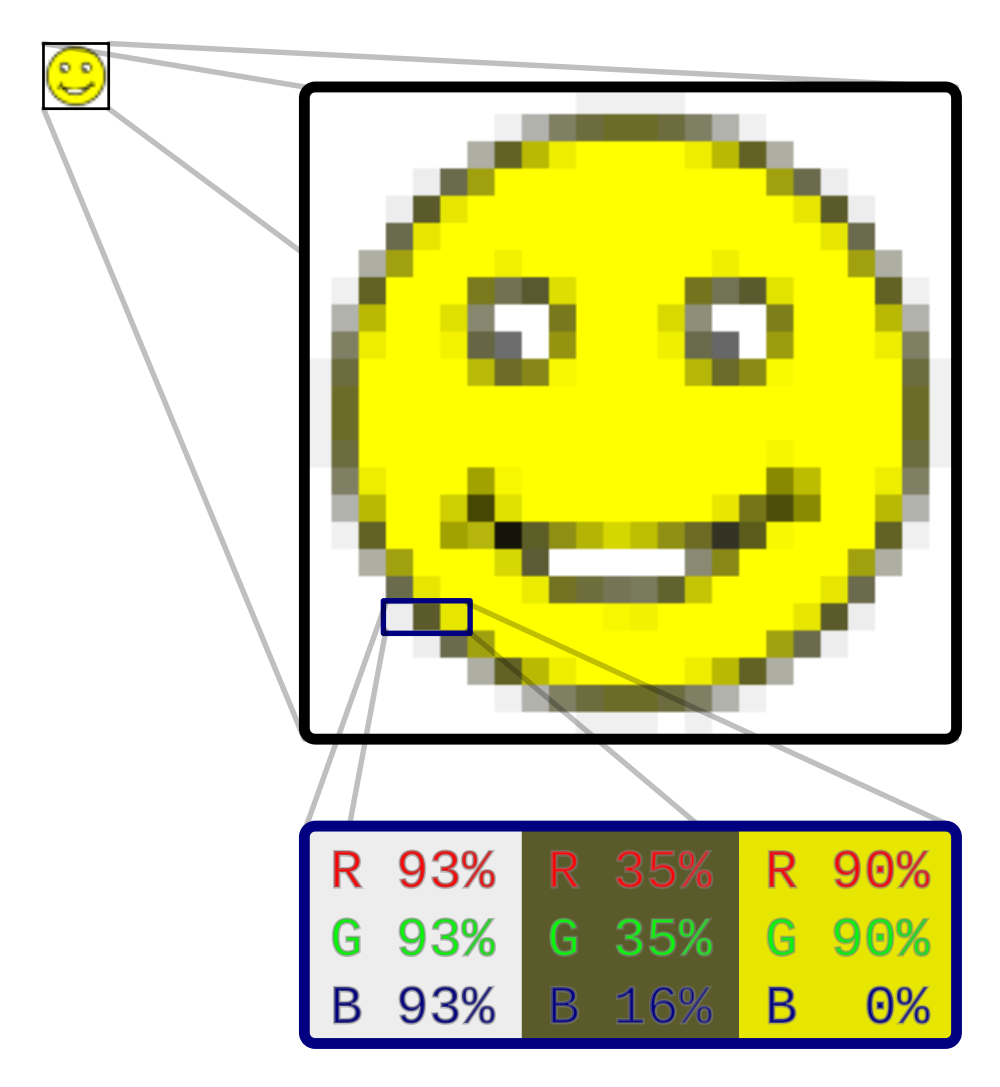
\includegraphics[width=0.6\textwidth]{src/images/rgb-raster-image.png}
  \caption[Example of an RGB raster image]{Example of a RGB raster image\protect\footnotemark}
  \label{fig:rgb-raster-image}
\end{figure}
\footnotetext{Source (accessed 02/2016): \url{https://en.wikipedia.org}.}

%explicit
\newpage

\subsection*{Human visual perception}

In his manuscript 'Astronomia Pars Optica' from 1604, Kepler explains the use of both eyes for depth perception.
He defined the term binocular as the composition of two latin words, 'bini' for double and 'oculus' for eye.
With uniocular as 'uni' for one the sight with only one eye is meant.
Binocular vision is then the vision creatures having two eyes obtain while using them together according to Kepler.
According to \citeauthor{fahle1987wozu} \citep{fahle1987wozu} and \citeauthor{henson2000visual} \citep{henson2000visual} creatures with binocular vision have several advantages over creatures with only uniocular vision.
Not to mention all but three, the most important ones which affect the depth perception:

\begin{enumerate}
  \item Considering human beings, the second eye increases the field of view \citep{henson2000visual}. About 120 degrees are the binocular field of view (projected on both eyes) and two uniocular fields of view with about 40 degrees.
  \item This also leads to another advantage with occluded, half-occluded or non-occluded objects \citep{fahle1987wozu}. Looking at Figure \ref{fig:horopter}, the point $P$ is in focus of the human being. Something directly behind this point may be fully occluded by the object in point $P$. Most of the things besides are non-occluded. Something behind this point $P$ may be half-occluded if it can be seen by either the left or the right eye.
  \item An advantage of having two eyes is the third-dimension human beings perceive, which leads to the binocular disparity or retinal disparity. Both terms are used in the literature and both mean the same: extracting depth information out of two coherent retinal images (obtained by the human eyes) \citep{cyganek2011introduction, fahle1987wozu}.
\end{enumerate}

\noindent Figure \ref{fig:horopter} depicts the mapping of the three points $R$, $P$ and $Q$ on the retina of each eye.
The letter $F$ stands for \textit{foveae} in which the visual axis ends.
The eye is constructed out of photoreceptor cells, mainly rods and cones.
The rods are necessary for seeing at night while the cones are responsible for humans being able to see the world sharp.
In the foveae is the peak of cones and it contains very few rods.
This means that the human visual system works the way that the visual axis joins the point of fixation with the foveae.
This can be seen in Figure \ref{fig:horopter} as the lines between $F$ of each eye to the point of fixation $P$.
Both eyes should be brought into convergence that the point of interest is projected onto the foveae of each eye.
Everything on the horopter (the circle) is corresponding (e.g. $P$ and $Q$), all points other than being on the horopter are non-corresponding ($R$) in terms of retinal disparity.
\newline\newline\noindent In the later described disparity algorithms which act like a tool for computers to be able to see the shift of pixels from the left image to the right image, the human being does somehow the same.
Humans experience the depth which is sensed unconsciously by the eyes and calculated by the brain in real-time.
With two eyes basically two slightly different images are obtained.
The brain acts as the computer which puts both coherent images together and extends the two-dimensional space into a three-dimensional space and calculates the position of the objects in the z-axis.

\begin{figure}[h!]
  \centering
  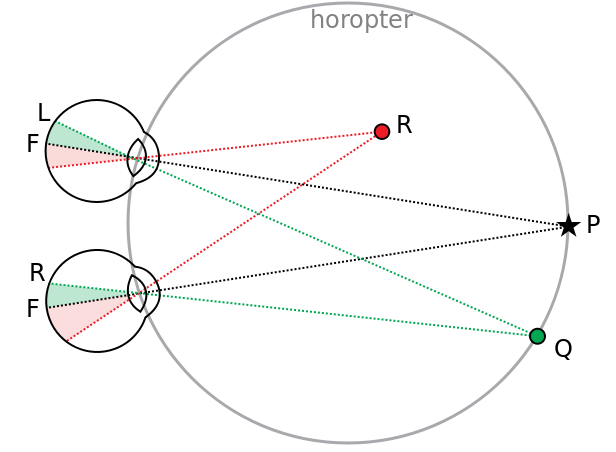
\includegraphics[width=0.6\textwidth]{src/images/horopter.png}
  \caption[Binocular vision with horopter principle]{Binocular vision with horopter principle\protect\footnotemark}
  \label{fig:horopter}
\end{figure}
\footnotetext{Source (accessed 02/2016): \url{https://en.wikipedia.org}.}

\noindent In contrast to the visual perception human beings perceive, computers need to do several steps to obtain disparity and calculate depth information:

\begin{itemize}
  \item identify objects,
  \item identify layers,
  \item match objects / pixels in both images,
  \item calculate the shift of the pixels from left to right, and
  \item obtain final depth values.
\end{itemize}

\noindent The human brain enables human beings to see and experience the real-world three-dimensional.
A computer has to be programmatically instructed to identify and group objects in both images \citep{block20133d, cyganek2011introduction}.
This is not an easy task as can be seen in the next sections.

\subsection*{Stereoscopy}

To paint the bigger picture, stereoscopy and the illusion of depth are introduced.
Stereoscopy is sometimes linked to the phrase 'the illusion of depth' as it is a technique used to add a third dimension to a flat image to simulate depth \citep{block20133d, lucas20133d}.
Specifically, the goal is to show each eye a slightly different image and thus achieve depth perception in our brain.
With so called stereoscope or special glasses depth perception can be transferred to the consumer in a cinema or at home via showing each eye a different image which then is composed to the final spatial perception.
\newline\newline\noindent There exist several techniques to create the stereoscopic effect. One of these glasses is the shutter system.
The concept of a shutter glass is that it cycles a block (meaning only one eye is dispatched to the screen) with a certain frequency (usually about 120 fps\footnote{frames per second}, resulting in 60 fps per eye) synchronously with the 3DTV.
This means that only one specific image is passed to exactly one of the consumers eyes.
So each eye is shown about 60 fps which naturally is experienced as flicker-free.
The older anaglyph 3D technique uses multiplied images tinted with red/cyan to filter out the respective image by the glasses filter foil, thus only one image is dispatched to one specific eye at a time.
Nowadays the anaglyph 3D technique is sometimes used in magazines to show 3D graphics.
As all techniques are not representing the real-world and the depth perception can be adjusted with for instance camera positioning (image one would reposition his eyes to perceive the real-world differently) they can be summarized as the illusion of depth.

\subsection*{Epipolar geometry}

The geometry of stereo images, called epipolar geometry, plays an important role in understanding the mathematical equations in the upcoming section.
The most important terms of epipolar geometry are:

\begin{itemize}
  \item image plane,
  \item baseline,
  \item epipole,
  \item epipolar line, and
  \item epipolar plane.
\end{itemize}

\noindent The \textit{image planes} in Figure \ref{fig:epipolar} and Figure \ref{fig:epipolar-rectified} are the blue surfaces which represent the captured image through the cameras $O_L$ and $O_R$.
The \textit{baseline} is the line joining both camera centers with the image plane. Focusing on the figures, the baseline is the line going from $O_L$ to $O_R$, as $O$ reflects the origin (camera center).
An \textit{epipole} is the joint of the baseline with the image plane, referring to the symbols $e_L$ and $e_R$.
The \textit{epipolar plane}, visualized as green triangle in Figures \ref{fig:epipolar} and \ref{fig:epipolar-rectified}, is determined by point $X$ and both origins $O_L$ and $O_R$.
It is the surface reflecting the z-axis, the depth.
An \textit{epipolar line} then is the intersection between the origin to the point of interest, in this particular case $X$, which lies on the epipolar plane and intersects the image plane.

\begin{figure}[h!]
  \centering
  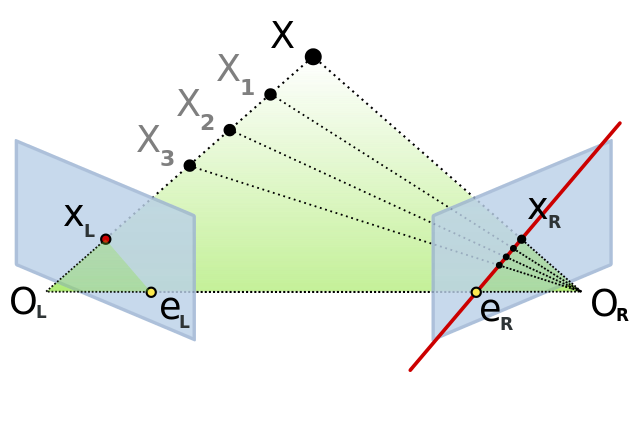
\includegraphics[width=0.7\textwidth]{src/images/epipolar.png}
  \caption[Epipolar geometry]{Epipolar geometry\protect\footnotemark}
  \label{fig:epipolar}
\end{figure}
\footnotetext{Source (accessed 02/2016): \url{https://en.wikipedia.org}.}

\noindent This results in an epipolar constraint \citep{cyganek2011introduction}:
Each image point $X_i$ of a space point in the image plane, e.g. consider point $X$ in Figure \ref{fig:epipolar} must lie on the corresponding epipolar line $\vec{O_LX}$.
More concrete focusing on Figure \ref{fig:epipolar}: this constraint states that the correspondence for a point on the epipolar line $\vec{O_LX}$ must lie on the line $\vec{e_rX_r}$.
As seen above Figure \ref{fig:epipolar} depicts the left and right view of an object in point $X$.
\newline\newline\noindent The Figures \ref{fig:epipolar} and \ref{fig:epipolar-rectified} both illustrate the epipolar geometry on a pair of unrectified images and the result after the rectification was done.
Rectification\footnote{Affine transformation (rotation and translation) neglecting geometric distortion to rectify the images.} is necessary to reduce the search-space from two-dimensional to one-dimensional.
For determining the exact position of $X$ (possible positions $X_i$ with $i = [1 \dots 3]$) the diagonal has to be scanned in the unrectified image.
In the rectified image only the horizontal needs to be investigated.
In the further proceeding this line is called the scanline which most of the algorithms operate on \citep{cyganek2011introduction, chowdhury2009new}.
After the rectification process the following two statements come true:

\begin{itemize}
  \item Epipolar lines are parallel to the x-axis (horizontal).
  \item Corresponding points are on the same y-axis (vertical).
\end{itemize}

\noindent Implicitly the following two assumptions were made:

\begin{itemize}
  \item the focal length $f$ of both cameras which captured the images are the same,
  \item the origin of one camera is the so called camera principal point (the joint of the optical axis with the image plane and the fovea counterpart) \citep{cyganek2011introduction}.
\end{itemize}

\noindent In conclusion, corresponding points are constrained to be on the same line and thus depth can be inferred by using triangulation and camera parameters.
Based on this, the investigations of stereo correspondence and the actual depth calculation using triangulation is discussed in more detail in the next sections.

\begin{figure}[h!]
  \centering
  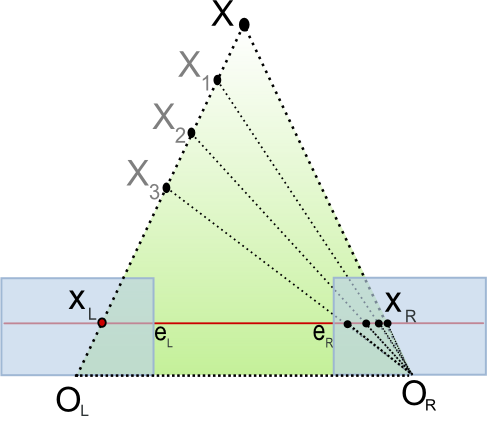
\includegraphics[width=0.6\textwidth]{src/images/epipolar-rectified.png}
  \caption[Epipolar geometry after image rectification]{Epipolar geometry after image rectification\protect\footnotemark}
  \label{fig:epipolar-rectified}
\end{figure}
\footnotetext{Source (accessed 02/2016): \url{https://en.wikipedia.org}.}

%explicit
\newpage

\section{Stereo correspondence}

Stereo correspondence can be seen as a pixel labelling problem \citep{wanner2013reconstructing, cyganek2011introduction} between two (or more) stereo images.
The essential problem is to find corresponding pixels in images of different cameras and needs to be solved.
Without knowing which points belong to each other in two separate stereo images, no conclusions can be drawn for instance calculating the disparity.
Henceforth, while talking about images for stereo matching, rectified images are implicitly meant.
If images are existing in an unrectified unaligned version then as a preprocessing step the images will be rectified.

\subsection*{Constraints}

Stereo matching algorithms rely on several assumptions about the real-world.
From the pioneer work of \citeauthor{marr1976cooperative} \citep{marr1976cooperative} the following constraints can be reasoned which are important for the development of such algorithms (also cf. \citep{cyganek2011introduction, wanner2013reconstructing,kack2004robust}):
\newline\newline\noindent \textit{As a short remark: $X_i$ is a point on a scanline in image $i$ ($i$ can be replaced with either $L$ for left or $R$ for right side) and thus only the x-position is mentioned.}

\begin{description}
  \item[Uniqueness] \hfill \\ As each pixel on a surface has one unique physical position in space, each pixel from each image has at most one disparity value.
  \item[Continuity] \hfill \\ The term smoothness constraint is also mentioned in the literature. Disparity can vary but smoothly almost everywhere in an image except at object boundaries which represent a discontinuity in depth, i.e. the difference of adjacent points should be small $||X_{L_1} - X_{R_1}| - |X_{L_2} - X_{R_2}|| < \varepsilon$.
  \item[Epipolar] \hfill \\ Recapture of the epipolar constraint from the section before: corresponding image points have to lie on the corresponding epipolar lines. If the epipolar lines are known to be parallel to the x-axis, the search space can be reduced to a 1D search space along the epipolar lines.
  \item[Ordering] \hfill \\ Following up the epipolar constraint: if the epipolar lines run in parallel to the x-axis, multiple consecutive image points have to lie on the same corresponding epipolar line in the same ordering.
  \item[Limit] \hfill \\ There is a defined disparity maximum (limit) $d_{max}$ holding $|X_L - X_R| < d_{max}$, defining the maximum disparity value which can be found in a stereo image. Hence, $d(x,y)$ is in the range $[0 \dots d_{max} - 1]$.
  \item[Lambertian] \hfill \\ Algorithms for stereo matching also rely on the assumption of opaque lambertian surfaces, meaning a surface that reflects light equally into all directions and thus appears equally bright independent from where light is coming and where the camera is placed. Thus the algorithms can expect the intensities and colors of corresponding points to be almost the same.
\end{description}

\noindent Besides those constraints there also exist some common pitfalls which can disturb the result of algorithm.

\subsection*{Common pitfalls}

Algorithms are using different metrics to analyze similarities in images along scanlines, in whole areas, or at a global view to then estimate the disparity.
This can be challenging especially considering the upcoming traps.
On the one hand, potential issues from the camera setup can be challenging, such as:

\begin{itemize}
  \item photometric distortions,
  \item noise,
  \item calibration error of the cameras.
\end{itemize}

\noindent On the other hand, the scenery can be tricky:

\begin{itemize}
  \item specularities and reflections,
  \item transparent objects,
  \item matching ambiguity,
  \item occlusions (missing data) and discontinuities.
\end{itemize}

\noindent These issues also challenge the algorithms to stereo match the pixels correctly.
With matching ambiguities, constant or low-contrast regions are meant.
A good example for that are textureless regions or repetitive structures.
Textureless regions could contain a small set of matching pairs of pixels, other pixels of that region could be erroneously assumed the same.
The presented constraints support the algorithms regarding those pitfalls.

\subsection*{Simplified stereo matching}

Figure \ref{fig:stereo-matching} depicts a simplified example of how stereo matching works on a one-dimensional search space:
there exist two arrays with $length = 5$, one in the left and one in the right image.
Assuming the top row $[p \dots t]$ reflects one row in the left image.
The bottom row $[u \dots y]$ accordingly the same row in the right image.
The pixel $p$, $q$, $w$ and $y$ are unmatched, e.g. occluded.
Having a function $d(z)$ which returns the disparity for a given element $z$ in those arrays, $d(r) = -2$ means the shift two to the left.
Accordingly $d(s) = -2$ and $d(t) = -1$.

\begin{figure}[h!]
  \centering
  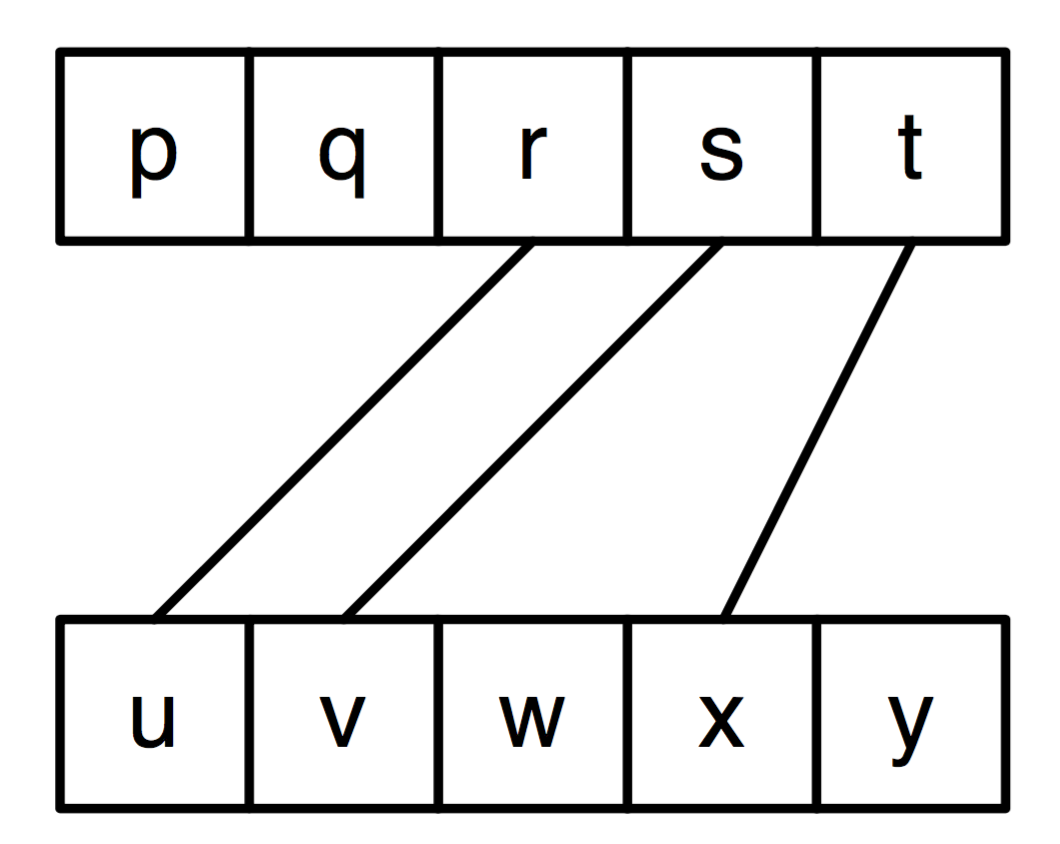
\includegraphics[width=0.3\textwidth]{src/images/stereo-matching.png}
  \caption[Two arrays illustrating stereo matching on a 1D search space]{Two arrays illustrating stereo matching on a 1D search space \citep{kack2004robust}.}
  \label{fig:stereo-matching}
\end{figure}

\noindent Up to this point the epipolar geometry and the challenge with stereo matching were introduced.
The upcoming section defines disparity, illustrates the disparity map, and the depth calculation.

\section{Disparity map between stereo images}

In the last two sections epipolar geometry and the problem with stereo correspondence were introduced.
In this section the focus is on the term disparity, how disparity can be visualized via disparity maps, and how the depth can be calculated out of those disparity values.

\subsection*{Disparity}

The disparity is the shift of a pixel / object (feature) between two or more images.
An object may appear at position $(x_1,y_1)$ in the left one and at position $(x_2,y_2)$ in the right one.
The disparity is the shift from the left position to the right one.
With $P_i$ declaring a point, left or right side, the following represents the disparity for two points in a two-dimensional space utilizing the pythagorean theorem:

\begin{equation}
  D(P_L,P_R) = \sqrt{D^2_X(P_L,P_R) + D^2_Y(P_L,P_R)}
\end{equation}

\noindent Henceforth, as the assumption of rectified images was made, only the horizontal disparity $D_X$ is meant by the term 'disparity'.

\begin{equation}
  D_X = |X_1 - X_2|
\end{equation}

\noindent In other words, having a pixel $(x_1,y_1)$ in a reference image (left) $l$ and a pixel $(x_2,y_2)$ in our matching image (right) $r$ the correspondence is given by:

\begin{equation}
  x_2 = x + |d(x_1,x_2)|\quad \textrm{with}\quad y_1 = y_2,
\end{equation}

\noindent where $d(x,y)$ is the function which delivers values out of the disparity space $(x,y,d)$ computed by the algorithms.
\newline\newline\noindent Resulting in matching pixels from one image to another, the disparity for each pixel-wise combination is calculated as seen in the previous subsection (simplified stereo matching) and presented here.
Such disparities can also be seen as the inversed distances to observed objects.
As a matter of fact, at the border of each image some pixels can not be calculated caused by the non-existing counterpart for matching.
Those pixels with no fellow are called 'occluded' pixels.
For example, in some cases pixels are hidden in one image by an object due to the blocking line of sight of this object.

\subsection*{Disparity map}

In order to actually analyze the output of algorithms ground-truth data is necessary.
An algorithm normally outputs a disparity map reflecting the disparity space $(x,y,d)$.
This disparity map can be seen as matrix having the size of the original image ($m \times n$) and containing values ranging from $0$ to $d_{max} - 1$ utilizing one color channel (grayscale).
The maximum disparity can be set via parameter for most of the algorithms and a feasible value which yields to sound results is $64$.
For better visual analysis the disparity maps are usually normalized to values ranging from $0 - 255$ \citep{martull2012realistic, cyganek2011introduction, scharstein2002taxonomy}.
Figure \ref{fig:tsukuba} c) shows the ground-truth data representing the disparity map.
The disparity map depicts grayscale intensities with lighter gray representing pixels / objects closer to the camera.
\newline\newline\noindent Tying in with the term ground-truth \citeauthor{martull2012realistic} created the first "highly realistic CG dataset that properly models real-world imperfections, while providing accurate ground truth." \citep{martull2012realistic}.
Without such datasets bad evaluation of stereo matching algorithms can be made as there would been no reference to evaluate against.
Figure \ref{fig:tsukuba} shows the previous dataset of the University of Tsukuba, the well-known \textit{Head and lamp scene}.

\begin{figure}[h!]
\centering
\begin{tabular}{ccc}
\subfloat[left input image]{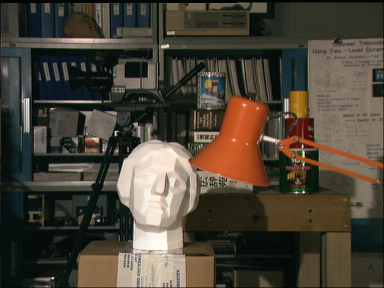
\includegraphics[width=0.3\textwidth]{src/images/tsukuba-imgL.png}} &
\subfloat[right input image]{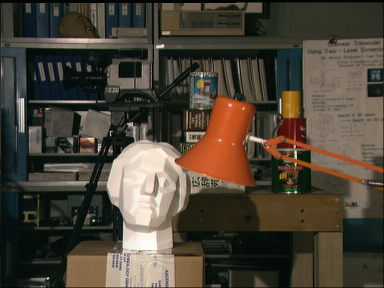
\includegraphics[width=0.3\textwidth]{src/images/tsukuba-imgR.png}} &
\subfloat[ground-truth data]{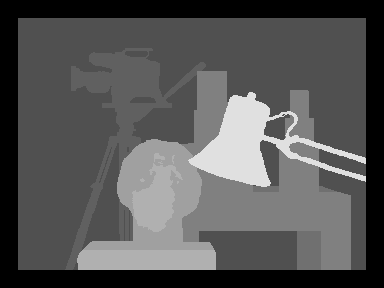
\includegraphics[width=0.3\textwidth]{src/images/tsukuba-dgt.png}}
\end{tabular}
\caption[Tsukuba benchmark stereo image pair of the University of Tsukuba]{Tsukuba benchmark stereo image pair of the University of Tsukuba \citep{martull2012realistic}.}
\label{fig:tsukuba}
\end{figure}

\noindent The input for a perfect algorithm would be the reference image (a) and the matching image (b).
After computation the result would be similar to the ground-truth data (c).
With evaluation metrics the computed disparity map is then compared to the ground-truth data.
Measuring instruments serve as a quality indicator for an algorithm's performance.
The above example is given for basic knowledge and understandability of how a disparity map actually looks like.
Details of this process are examined in the evaluation Chapter \ref{chap:eval}.

\subsection*{Depth calculation}

From an obtained disparity map and given camera parameters the depth can be calculated.
The mathematical description of the following equations has been introduced by \citeauthor{cyganek2011introduction} in Chapter 3.4.9 (Depth Resolution in Stereo Setups) of their book "\textit{An introduction to 3D computer vision techniques and algorithms}" \citep{cyganek2011introduction}.
Assuming the focal length of the camera's lens and the baseline\footnote{The distance between both image sources.} are known, the following holds:

\begin{equation}
  Z = \frac{f \cdot B}{d}\quad \textrm{and}\quad d = \frac{f \cdot B}{Z}
\end{equation}

\begin{equation}
  X = \frac{x \cdot Z}{f}\quad \textrm{and}\quad Y = \frac{y \cdot Z}{f}
\end{equation}

where:

\begin{itemize}
  \item $Z$ is the distance along the z-axis (camera axis),
  \item $f$ is the focal length,
  \item $B$ is the baseline (in meters),
  \item $d$ is the disparity of the point.
\end{itemize}

\noindent After $Z$ is determined, $X$ and $Y$ can be calculated using the usual projective camera equations (2.4-2.5) where the point $(x,y)$ is the pixel location in the 2D reference image and $(X,Y,Z)$ describes the real 3D position \citep{scharstein2002taxonomy, cyganek2011introduction, block20133d, martull2012realistic}.
Figure \ref{fig:depth-estimation} depicts the depth calculation from disparity with $X$ being the estimated point and $d = x - x'$.
\newline\newline\noindent The following subsection describes the more general steps of how disparity algorithms work, known as the taxonomy.

\begin{figure}[h!]
  \centering
  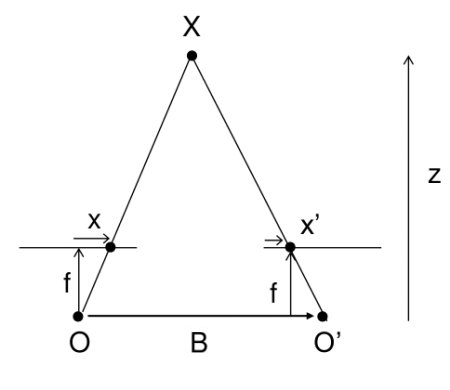
\includegraphics[width=0.6\textwidth]{src/images/depth-calculation.png}
  \caption[Depict of depth calculation from disparity.]{Depict of depth calculation from disparity.\protect\footnotemark}
  \label{fig:depth-estimation}
\end{figure}
\footnotetext{Source (accessed 02/2016): \url{http://docs.opencv.org}.}

%explicit
\newpage

\section{Disparity algorithms}

In the last sections different aspects affecting stereo matching were introduced.
To get a better understandability of the algorithm's technique, this section focuses on the diversity and taxonomy of disparity algorithms.

\subsection*{Diversity of disparity algorithms}

A lot of different algorithms exist and their workings differ slightly.
According to \citeauthor{cyganek2011introduction} \citep{cyganek2011introduction}, \citeauthor{scharstein2002taxonomy} \citep{scharstein2002taxonomy}, the following categories to separate disparity algorithms exist.
Some of these classifications are discussed in more detail the related work Chapter \ref{chap:related}.
\newline\newline\noindent First, the output of an algorithm is rated: they can create sparse or dense disparity maps.
On the one hand, most of the algorithms produce a dense disparity map meaning that almost every pixel got a corresponding shift value.
On the other hand, sparse algorithms only calculate values around, for instance, feature points (cf. feature matching).
One advantage of sparse algorithms compared to dense disparity algorithms is that they are normally faster in computation but limited in applications.
Approaches to interpolate sparse disparity maps into dense disparity maps exist, but they tend to produce inaccurate results in comparison to dense algorithms.
\newline\newline\noindent Second, \citeauthor{cyganek2011introduction} \citep{cyganek2011introduction} categorize direct and indirect methods.
Indirect methods are feature based or operate in the transformed image space (cf. Chapter 6.3.7 in \citep{cyganek2011introduction}).
Direct methods use intensity based measures.
\newline\newline\noindent Finally, disparity algorithms are classified into local and global methods:

\begin{itemize}
  \item Local Methods
  \begin{itemize}
    \item Feature matching
    \item Block (area) matching
  \end{itemize}
  \item Global Methods
  \begin{itemize}
    \item Belief propagation
    \item Graph cuts
    \item Dynamic programming
    \item Layering (hierarchical scale-space)
  \end{itemize}
\end{itemize}

\subsection*{Taxonomy of disparity algorithms}

\noindent Assumptions need to be made before starting to describe the taxonomy of disparity algorithms:

\begin{enumerate}
  \item The algorithm is fed with a pair of rectified images as input.
  \item The algorithm produces a dense integer disparity map, which means that disparity is estimated at each pixel.
  \item Most of the current algorithms works according to the following steps (see Figure \ref{fig:disparity-flow})
\end{enumerate}

\tikzstyle{rblock} = [text width=10em, rectangle, draw, fill=blue!20, text centered, rounded corners, minimum height=3em]
\tikzstyle{cloud} = [text width=6.5em, ellipse, draw, fill=red!15, text centered, rounded corners, minimum height=3em]
\begin{figure}[h!]
  \centering
  \begin{tikzpicture}[node distance=4.8em, auto]
    \node [cloud] (input) {Pair of rectified images};
    \node [rblock, below of=input] (matchingcost) {Computing the matching cost};
    \node [cloud, below of=matchingcost] (DSI) {Disparity space image};
    
    \node [rblock, right of=computation, below of=DSI, node distance=6em] (aggregation) {Aggregation of the cost values};
    \node [rblock, left of=aggregation, below of=DSI, node distance=6em] (computation) {Computation of the disparity};    
    
    \node [cloud, below of=DSI, node distance=12em] (disparity) {Disparity map};
    \node [rblock, below of=disparity] (refinement) {Disparity refinement};

    \path [line] (input) -- (matchingcost);
    \path [line] (matchingcost) -- (DSI);
    \path [line] (DSI) -- node[anchor=north, xshift=-4.8em, yshift=1.0em] {for global methods}(computation);
    \path [line] (DSI) -- node[anchor=north, xshift=4.8em, yshift=1.0em] {for local methods}(aggregation);
    \path [line] (aggregation) -- (disparity);
    \path [line] (computation) -- (disparity);
    \path [line] (disparity) -- (refinement);
  \end{tikzpicture}
  \caption[Basic processing flow of typical disparity algorithms]{Basic processing flow of typical disparity algorithms, cf. \citep{cyganek2011introduction, scharstein2002taxonomy}.}
  \label{fig:disparity-flow}
\end{figure}

\noindent The upcoming subsections discuss the steps in more detail, especially regarding the computation of the matching cost and the subsequent aggregation.

%explicit
\newpage

\subsubsection{Matching cost functions}

At first, the similarities of pixels in both images are calculated.
In general, the literature shows matching cost as the dissimilarities of pixels.
The matching cost needs to be computed for the decision which pixel belongs to another.
Hence, the cost needs to be low for similar pixels.
Some of the matching criteria used for determining the matching cost are described in Table \ref{tab:overview-matching-cost-functions} cf. \citep{cyganek2011introduction, scharstein2002taxonomy, opencv_library, kanade1995development, hamzah2010sum}.

\begin{table}[h!]
\centering
\begin{tabular}{l|l}
  \hline
  \textbf{Method} & \textbf{Formula} \\ \hline \hline
  Sum of absolute differences & $\displaystyle \sum_{i,j \in U} \left| I_1(x_L+i,y_L+j) - I_2(x_R+i,y_R+j) \right|$ \\
  Sum of squared differences & $\displaystyle \sum_{i,j \in U} (I_1(x_L+i,y_L+j) - I_2(x_R+i,y_R+j))^2$ \\
  Normalized cross-correlation & $\displaystyle \frac{1}{n} \sum_{x,y}\frac{(I_1(x_L,y_L) - \overline{I_1})(I_2(x_R,y_R) - \overline{I_2})}{\sigma_{I_1} \sigma_{I_2}}$ \\
  \hline
\end{tabular}
\caption{Most common similarity measures}
\label{tab:overview-matching-cost-functions}
\end{table}

\noindent $I_k(x,y)$ stands for an intensity value of the image $k$ at the point with given coordinates $(x,y)$.
The set $U = U(i,j)$ describes close-by points located around the point $(i,j)$.
The sum of absolute differences (SAD) similarity measure is one of the simplest ones and describes the difference between pixel values.
The absolute intensity differences of both images $I_1$ and $I_2$ are summed up for all adjacent pixels in the neighborhood (described with $U$).
Zero stands for the equality of both regions.
In optimal images nearly every pixel in the left image should have a corresponding pixel in the right image, fulfilling the constraints from the section before, and thus the calculated SAD should sum up to zero.
The lower the result, the more similar the pixels and the cheaper the matching cost are.
\newline\newline\noindent In the sum of squared differences (SSD) similarity measure the pixel differences are squared and summed up.
This measurement needs a bit more computational power and is usually chosen to discriminate high differences.
It can yield to better results if outliers need to be excluded and the difference is not strong enough while using SAD.
\newline\newline\noindent There also exist the normalized cross-correlation (NCC).
Cross-correlation measures the correlation between two intensity values in a point $(x,y)$.
The normalized cross-correlation subtracts the mean $\overline{I}$ of the intensities and divides by the standard deviation $\sigma_{I}$ to normalize the intensity values. This may be necessary to balance brightness variations.
NCC is excluded in most scientific investigations regarding disparity algorithms as it behaves similar to SSD (cf. \citep{hirschmuller2007evaluation, scharstein2002taxonomy, cyganek2011introduction}).

%explicit
\newpage

\subsection*{Disparity space image}

Related to the disparity space introduced in the section before, the disparity space image (DSI) should be defined.
The DSI is an image or a function over a continuous or discretized version of the disparity space $(x,y,d)$ and represents the matching cost (i.e. the dissimilarity) of a given $d(x,y)$.
It can be imagined as a three-dimensional matrix with the x-axis meaning the column, the y-axis the disparity and each combination the matching cost for that particular value as the z-axis.
The disparity space image $C(x,y,d)$ is the result of the matching cost values over all pixels and all disparities, where the function $C$ that denotes the matching cost for the given input parameter.
This leads to the aggregation step, during which the matching cost form the final disparity for local methods.

\begin{figure}[h!]
  \centering
  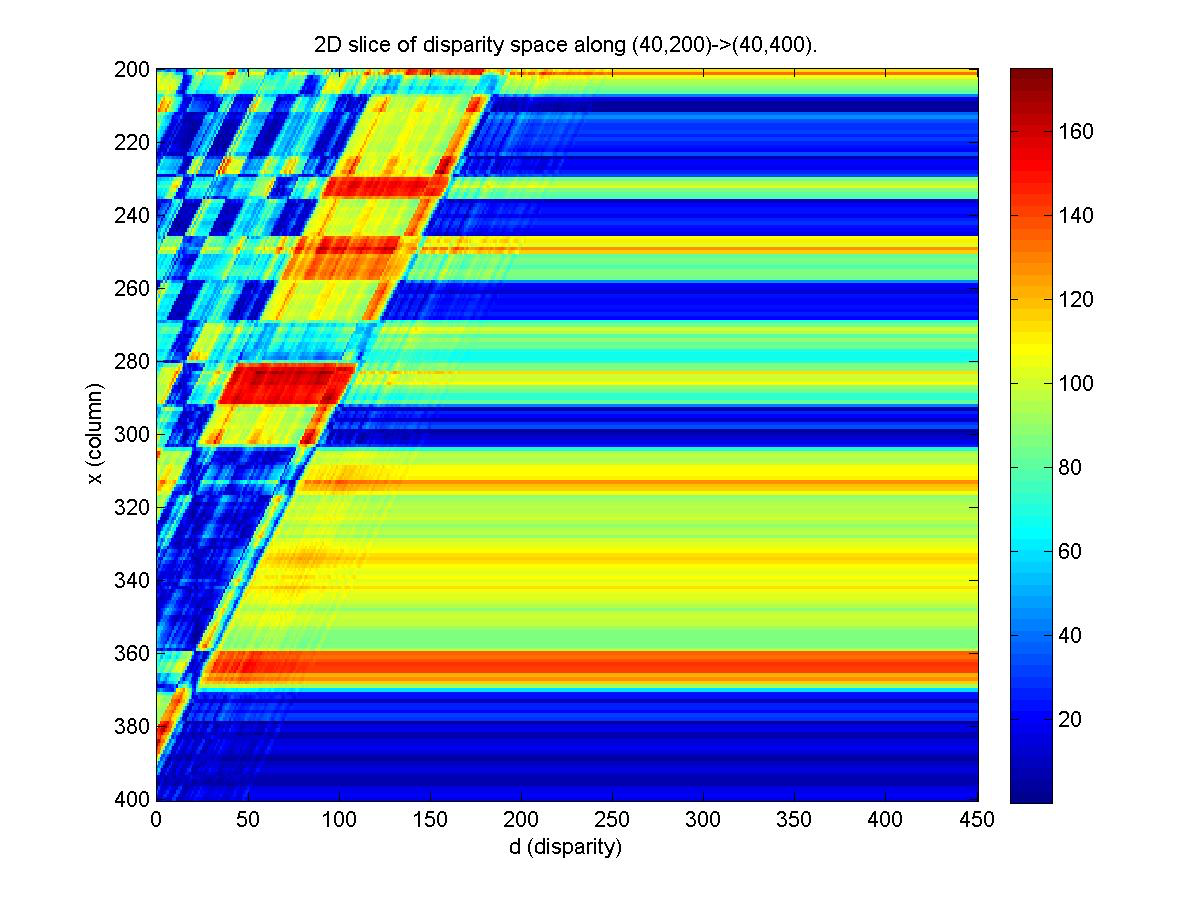
\includegraphics[width=1.0\textwidth]{src/images/dsi.png}
  \caption[Disparity space image]{Illustration of a disparity space image.\protect\footnotemark}
  \label{fig:dsi}
\end{figure}
\footnotetext{Source (accessed 03/2016): \url{http://www.cs.virginia.edu/~cab6fh/CV_4/WRITEUP.html}.}

\subsubsection{Aggregation}

In the aggregation step the decision has to be made, which discrete set of disparities represents the scene best \citep{scharstein2002taxonomy}.
As the matching cost values over all pixels and all disparities are stored in the DSI the minimum for each row is chosen as the best matching pixel and thus declared as the corresponding pixel.
In other words: for every pixel the disparity with the lowest cost is selected.
This strategy is known as the winner takes it all (WTA). \citep{cyganek2011introduction, scharstein2002taxonomy}.
As the pixel with the lowest cost is chosen, the following holds:

\begin{equation}
  d(x,y) = \arg\min_{d'} C(x,y,d').
\end{equation}

\subsubsection{Disparity computation}

After the aggregation, the actual disparity is computed in this step.
It is split up for the two different methods: local and global.
\newline\newline \noindent \textbf{(i) Local methods.} Local methods focus on the matching cost computation and the cost aggregation steps.
The final disparity computation is trivial as the minimum cost value (least dissimilarities) over each row is chosen (WTA).
\newline\newline\noindent \textbf{(ii) Global methods.} In contrast to local methods, global methods unify the three basic steps into a single one by defining an energy function to be minimized.
It ties in with the labelling problem \citep{tamassia2013handbook}.
A row in the DSI can be imagined as the different labels (i.e. disparity values) one pixel can receive.
The labelling problem describes the search of the disparity as the choice of the correct label.
Each pixel should only have one label assigned in the end.
\newline\newline\noindent Let $P$ be a set of pixels and $D$ a set of disparities. The energy function aims to find a disparity $d$ which minimizes some energy:

\begin{equation}
  E(d) = E_{data}(d) + \lambda E_{smooth}(d).
\end{equation}

\noindent The data term $E_{data}(d)$ defines the matching cost for a given disparity function $d$ and expresses how well the disparity function $d$ matches with the input image pair.
$C$ is the matching cost DSI:

\begin{equation}
  E_{data}(d) = \sum_{(x,y)} C(x,y,d(x,y)).
\end{equation}

\noindent As each pixel should be matched to a good find in the other image but simultaneously the adjacent pixels should be normally piecewise smooth, i.e. about the same value / intensity, the smoothness term $E_{smooth}(d)$ is introduced to reflect that (cf. stereo correspondence constraints).
The $\lambda$ is introduced to control how much the smoothness term should influence the overall data term.
To make the smoothness term computationally affordable it is, depending on the algorithm, usually restricted on the differences between adjacent pixel disparities \citep{scharstein2002taxonomy, cyganek2011introduction}, i.e. the disparity gradient:

\begin{equation}
  E_{smooth}(d) = \sum_{(x,y)} p(d(x,y) - d(x+1,y)) + p(d(x,y) - d(x,y+1)),
\end{equation}

\noindent where $p$ is a "monotonically increasing function of disparity difference" \citep{scharstein2002taxonomy}.
Depending on the used algorithm, other smoothness term functions exist.
The optimization problem to solve is defined as the minimization of the energy function, i.e.:

\begin{equation}
  D = \arg\min_{d} E(d),
\end{equation}

\noindent where $D$ is the disparity map containing the final values for every $(x,y)$ and $d$ a set of parameters or a disparity function affecting the energy value.
\newline\newline\noindent The search space for finding a solution is large, as an $n \times m$ image with $k$ disparities has about $k^{n \times m}$ possible solutions.
According to \citeauthor{scharstein2002taxonomy} \citep{scharstein2002taxonomy}, \citeauthor{cyganek2011introduction} \citep{cyganek2011introduction} finding the global minimum is \textit{NP-hard}.
The related work in Chapter \ref{chap:related} gives an introduction into solving those optimization problems.

\subsubsection{Disparity refinement}

Disparity refinement can be seen as an optional post-processing step some algorithms perform automatically or may be requested manually.
Refinement steps can also be implemented independently from the algorithm as they are executed on the final disparity maps.
Sometimes the literature mentions those as clean-up steps.
Here is a list of some known refinement steps:

\begin{itemize}
  \item Sub-pixel estimation for higher accuracy.
  \item Disparity verification with left-to-right and right-to-left disparity map comparison (can also detect occluded areas).
  \item Filtering of disparity values, for instance using a median filter to remove mismatches.
  \item Interpolation of missing values: can be necessary when using an algorithm which produces a sparse disparity map.
\end{itemize}

\subsubsection{Simplified block matching}

\noindent For demonstration purpose of a working local disparity algorithm, block matching, also known as area matching, is sketched in a simplified version.
The following algorithm assumes rectified images.
Thus, the algorithm is executed along the scanlines.

\begin{enumerate}
  \item Divide the images in blocks of the size $m \times n$ (e.g. $8 \times 8)$.
  \item Find the corresponding block along the scanlines as shown in Figure \ref{fig:tsukuba-block}, i.e. the block with the lowest matching cost (e.g. sum of absolute differences).
  \item Calculate for this block the displacement (the shift from left to right image) which results in the disparity.
  \item This yields in the final, ideally \textit{bijective}\footnote{Considering two sets, for each element of the first set a corresponding element of the second set is found. It also holds that both sets contain the same amount of elements. Thus, it is a one-to-one correspondence which also works inversely.} disparity map after finding the corresponding block from the left to the right image and vice versa. If a block could not be matched the bijective criteria is not fulfilled.
\end{enumerate}

\begin{figure}[h!]
  \centering
  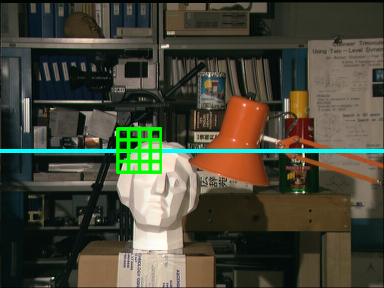
\includegraphics[width=0.5\textwidth]{src/images/tsukuba-block.png}
  \caption{Illustration of block matching along a scanline.}
  \label{fig:tsukuba-block}
\end{figure}

\noindent In general, block matching leads to more accurate results with smaller window sizes.
A bigger window leads to more smoothing which results in lower noise.
The window size depends on the image size and its content.
Therefore, no general assumption can be made.
For each scenery the window size should be adjusted individually.

\section{Sub-pixel accuracy}

As seen in the sections before, the disparity algorithms produce a disparity map consisting of integer values only.
For most of the imaginable applications integer values should be enough.
However, the world is continuous and there are applications which rely on accurate disparity estimations.
For instance, having no sub-pixel values, image-based rendering produces an image for visualizing the disparity map, which can appear to be made up of many thin shearing layers \citep{scharstein2002taxonomy}.
To get an accurate sub-pixel value, the most common technique is to use curve fitting by utilizing an \textit{n-th} polynomial-order function.
In this particular case \citep{scharstein2002taxonomy}, a second-order polynomial function, i.e. a parabola is used.
The curve is fitted around three or more values of the matching measure.
The point of interest lies in the center of the chosen window (as Figure \ref{fig:sub-pixel-estimation} depicts).
The minimum of this parabola is the searched value \citep{cyganek2011introduction, scharstein2014high}.
\newline\newline\noindent Curve fitting with a second-order-polynomial in Figure \ref{fig:sub-pixel-estimation} works with three data points: $(d_{i-1}, m_{i-1})$, $(d_{i}, m_{i})$ and $(d_{i+1}, m_{i+1})$.
$d_i$ is the found integer value for disparity and $m_i$ is a match value for the displacement $d_i$.
With the curve fit a new minimum value $d_x$ is found which no longer needs to lie on the integer grid.

\begin{figure}[h!]
  \centering
  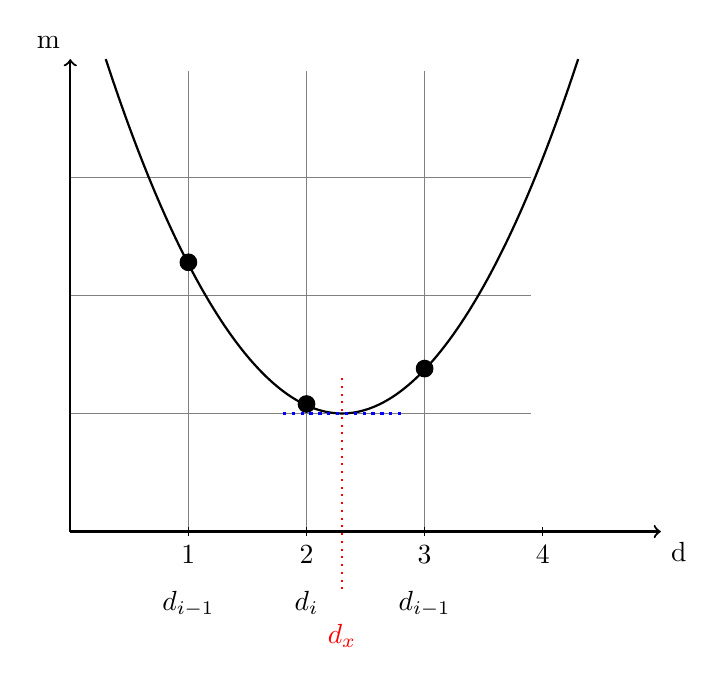
\begin{tikzpicture}[scale=1.5]
    %grid
    \draw[step=1cm,gray,very thin] (0,0) grid (3.9,3.9);
    %axes
    \draw[thick,->] (0,0) -- (5,0) node[anchor=north west] {d};
    \draw[thick,->] (0,0) -- (0,4) node[anchor=south east] {m};
    \foreach \x in {1,2,3,4}
      \draw (\x cm,1pt) -- (\x cm,-1pt) node[anchor=north] {$\x$};
    \draw (1cm,-12pt) node[anchor=north] {$d_{i-1}$};
    \draw (2cm,-12pt) node[anchor=north] {$d_{i}$};
    \draw (3cm,-12pt) node[anchor=north] {$d_{i-1}$};
    
    \draw[red] (2.3cm,-20pt) node[anchor=north] {$d_x$};
    %parabola
    \draw[thick] (2.3,1) parabola (0.3,4);
    \draw[thick] (2.3,1) parabola (4.3,4);
    %points
    \draw (1,2.28) circle[radius=2pt];
    \fill (1,2.28) circle[radius=2pt];
    \draw (2,1.08) circle[radius=2pt];
    \fill (2,1.08) circle[radius=2pt];
    \draw (3,1.38) circle[radius=2pt];
    \fill (3,1.38) circle[radius=2pt];
    %lines
    \draw[dotted,blue,very thick] (1.8,1) -- (2.8,1);
    \draw[dotted,red,thick] (2.3,1.3) -- (2.3,-0.5);
  \end{tikzpicture}
  \caption{Sub pixel estimation of a disparity value around adjacent pixels.}
  \label{fig:sub-pixel-estimation}
\end{figure}

\section{Optical flow}

Similar to the problems discussed in the section before, optical flow is also an image matching problem.
The optical flow is defined as vectors describing small local displacements like moving objects or camera motion between two consecutive frames \citep{cyganek2011introduction, opencv_library}.
The principle of the matching problem of images is comparable to disparity algorithms.
The main difference is that instead of analyzing left and right image, a scene is investigated and the disparity describes small local vectors.
To be more precise, the optical flow relies on the assumption that a certain point $(x_1, y_1)$ in a frame at time $t_1$ will be matched to a point $(x_2, y_2)$ in a frame at time $t_2$.
Different approaches for estimating the optical flow of pixels exist, like:

\begin{itemize}
  \item Correlation or block-matching,
  \item feature tracking,
  \item energy-based methods, or
  \item gradient-based methods.
\end{itemize}

\noindent Optical flow is heavily used in autonomous driving, automated traffic surveillance systems and video compression like H.264 \citep{cohen1999detecting, richardson2004h, kondermann2015stereo, menze2015object}.
Recently a dataset containing ground-truth data of real-world sceneries regarding optical-flow information was released by \citeauthor{kondermann2015stereo}.
Figure \ref{fig:optical-flow-estimation} shows an example of estimating the movement of a vehicle.
In the left image of Figure \ref{fig:optical-flow-estimation} most of the vectors are null as no local displacement can be estimated.
Only a few vectors (small white dots) near the vehicle illustrate the displacements.

\begin{figure}[h!]
  \centering
  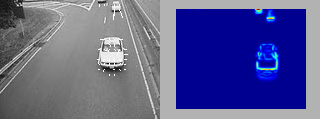
\includegraphics[width=1.0\textwidth]{src/images/optical-flow-estimation.jpg}
  \caption[Optical flow estimation]{Optical flow estimation to obtain motion vectors (left) and pixel velocity magnitudes (right).\protect\footnotemark}
  \label{fig:optical-flow-estimation}
\end{figure}
\footnotetext{Source (accessed 02/2016): \url{http://de.mathworks.com/discovery/optical-flow.html}.}


\chapter{Related work}
\label{chap:related}

In this chapter the related work regarding disparity algorithms is treated.
As integration of some disparity algorithms for the later evaluation was part of this thesis, the ones which were actually implemented are examined in more detail.
The well-known semi-global matcher by \citeauthor{hirschmuller2005accurate}, also implemented in the OpenCV library \citep{opencv_library}, is introduced.
OpenCV\footnote{\url{http://opencv.org}} is an extensive image processing framework, with the main goal towards real-time computer vision.
\citeauthor{Geiger2010ACCV} introduce an approach that enables fast matching of high-resolution images, which is also outlined in the upcoming section.
Both approaches utilize local methods for estimating disparity maps.
One candidate adopting global methods is the Middlebury MRF library, which is also introduced.
It implies solving optimization problems (i.e. the minimization of a global energy cost function).
The library’s implemented methods to solve such optimization problems are outlined in greater detail.
In the end, an outlook on disparity algorithms on stereoscopic videos is given, which includes an approach towards spatiotemporal consistency and remapping of the disparity range.

\section{Semi-global matching}

\citeauthor{hirschmuller2005accurate} combines two different methods, global- and local-matching for determining accurate disparity at a lower runtime as other global algorithms,  which are time consuming even on current hardware \citep{hirschmuller2005accurate, hirschmuller2008stereo}.
\newline\newline\noindent The semi-global matching (SGM) method utilizes pixel-wise matching of so called mutual information (MI) via entropy $H$.
The joint entropy of two images $I_1$ and $I_2$ results from the sum of their combined entropy and a global two-dimensional smoothness constraint $H_{I_1,I_2}$ which leads to the following cost:

\begin{equation}
  MI_{I_1,I_2} = H_{I_1} + H_{I_2} + H_{I_1,I_2}.
\end{equation}

\noindent The discussed one-dimensional constraints from Chapter \ref{chap:foundations} are applied as well.
Calculating the matching cost based on mutual information is insensitive to different video recording conditions and illumination changes \citep{hirschmuller2005accurate, viola1997alignment}.
The joint entropy $H_{I_1,I_2}$ is low (meaning low information content) for rectified images as one image can be predicted by the other.
The MI matching cost is defined as the following:

\begin{equation}
  mi_{I_1,I_2}(i,k) = h_{I_1}(i) + h_{I_2}(k) - h_{I_1,I_2}(i,k),
\end{equation}

\noindent where $h_1$ and $h_2$ are calculated from the probability distribution of corresponding intensities.
Thus, $h_{I_1,I_2}(i,k)$ serves as the matching cost for the two intensities $i$ and $k$.
The idea is, that one image needs to be warped\footnote{In this context warping can be seen as a function which maps pixels from the destination image to pixels in the original image. Then the pixels are copied at the mapped position to the coordinates in the destination image.} such that corresponding pixels are at the same location in both stereo images:

\begin{equation}
    I_1 = I_b\quad \textrm{and}\quad I_2 = f_D(I_m),
\end{equation}

\noindent where $I_b$ is the base image, $I_m$ the match image and $f_D(x)$ is a function which outputs the matching corresponding point.
As the matching cost represents the information content of two intensities $I_1$ and $I_2$, which should be low (i.e. matching parts are as equal as possible), the disparity map $D$ needs to be known \textit{a priori} for warping.
Hence, the MI matching cost needs to be calculated either iteratively or hierarchically.
On the one hand, an iteratively approach utilizes a random disparity image for calculating the MI matching cost, which serves as the base for the next iterations.
On the other hand, the MI matching cost can be calculated hierarchically by recursively using an up-scaled disparity image, which has been calculated at half resolution with a common similarity measurement like SAD.
For a deeper explanation of how the mutual information are exactly calculated and used in the SGM method compare \citep{hirschmuller2005accurate, hirschmuller2007evaluation, hirschmuller2008stereo, hirschmuller2011semi}.

\subsection*{OpenCV BM and SGBM}

The OpenCV library \citep{opencv_library}, currently at version 3.1.0, offers two implementations for disparity estimation, block matching and semi-global block matching based on the idea of \citeauthor{hirschmuller2005accurate}.
This latest version also contains a new filter, which was initially introduced with version 3.0.0, named \textit{Disparity WLS Filter}\footnote{\url{http://docs.opencv.org/3.1.0/d9/d51/classcv_1_1ximgproc_1_1DisparityWLSFilter.html}}.
WLS stands for weighted least squares (in the form of a fast global smoothing algorithm).
This disparity filter smoothes the disparity and also performs a left-right-consistency check to refine the results in especially half-occluded and uniform areas \citep{min2014fast}.
This yields to better and more accurate results but has the drawback of loosing negative disparity values.
Negative disparity appears if the stereo cameras are verged or inclined towards each other.
The WLS filtering results in disparity ranging from $0$ to $D_{max}$, which is set beforehand as a parameter.
Thus the negative disparity is $-1$.

\section{ELAS: Efficient large-scale stereo matching}

\citeauthor{Geiger2010ACCV} propose a novel approach for estimating the disparity with so called support points \citep{Geiger2010ACCV, Geiger2011IV}.
A support point is like a feature, a point which can be robustly matched.
For those support points, a sparse disparity map is calculated.
For more robustness, only the support points which can be matched left-to-right and right-to-left are retained.
To remove ambiguities, the ratio between the best and the second best match of all points is taken into account.
If the ratio exceeds a fixed threshold, the points are removed.
A support point which has a different disparity value than all its neighbor (adjacent) points is categorized as an outlier and removed as well.
As the found support points may not cover the whole image, additional support points in the image corners are added.
They adopt the disparity value of their nearest neighbor.
Then, image coordinates of the remaining support points are used to create a 2D mesh via Delaunay triangulation.
To obtain a dense disparity map, missing disparities are interpolated using mesh of the Delaunay triangulation by using the nearest-neighbor on the same image line.
For more information how the support points are calculated and how the interpolation is done exactly, compare \citep{Geiger2010ACCV, Geiger2011IV}.

\section{Middlebury MRF library}

The Middlebury MRF library \citep{scharstein2014high, szeliski2008comparative} utilizes a global energy function consisting of Markov random fields to formulate an energy minimization problem and offers the following methods to solve this optimization problem:

\begin{enumerate}
  \item iterated conditional modes (ICM),
  \item graph cuts expansion approach (cf. \citep{boykov2001fast, ramin2004energy, kolmogorov2004energy}),
  \item graph cuts swap approach (cf. \citep{boykov2001fast, ramin2004energy, kolmogorov2004energy}),
  \item sequential tree-reweighted max-product message passing (TRWS)\\(cf. \citep{kolmogorov2006convergent, wainwright2005map}),
  \item sequential belief propagation (BPS) (cf. \citep{boykov2001fast}),
  \item max-product belief propagation (BPM) (cf. \citep{boykov2001fast}).
\end{enumerate}

\noindent The following subsections give a rough overview on some of those methods.
Additionally, a short introduction into MRF-based energy functions is given.
Finally, a general outline of the concepts, that are utilized by the above mentioned techniques to solve such optimization problems, is given.

\subsection{Solving optimization problems}

Many problems in computer vision, for instance image smoothing, can be described in terms of energy minimization.
The stereo correspondence problem is formulated as described in Chapter \ref{chap:foundations}.
Thus, solving of optimization problems is a key part in modern stereo matcher algorithms.
They solve the labelling problem as described in Chapter \ref{chap:foundations}.
Most of the current disparity algorithms employ global methods to solve an energy minimization problem.
Usually they utilize Markov random fields (MRF) based energy functions.

As these are \textit{NP-hard}, approximation algorithms are typically used, like \citep{tappen2003comparison, cyganek2011introduction}:

\begin{itemize}
  \item dynamic programming,
  \item belief propagation,
  \item graph cuts.
\end{itemize}

\noindent All of these methods are supposed to solve inference problems, or at least provide approximated solutions.
Markov random fields, mentioned before, are also known as Markov network.
Bayesian networks as well as Markov networks are so called graphical models.
Such graphical models help to understand the reasoning behind those formulations and to actually build algorithms which solve those inference problems.
Both networks express the dependencies of nodes as the conditional probability.
A chain of nodes is called the joint probability\footnote{The joint probability $P(A \land B)$ is the probability of event A and event B occurring. It is the probability of the intersection of two or more events.}.
This then is the product over-all probabilities.
The goal of algorithms which solve inference problem is to compute certain marginal probabilities\footnote{The marginal probability is an unconditional probability as it is not conditioned on another event.}, i.e. the probability that some pixel reach a specific label node \citep{cyganek2011introduction}.
With inference the computation of these marginal probabilities is meant.
Marginal probabilities are defined as the sums over all possible states of all the other nodes in the system.
They are also called beliefs \citep{yedidia2003understanding}.

\subsubsection{Markov random fields}

Markov random fields (MRF), also called Markov network, are used to formulate problems in a probabilistic way.
The problem thereby is represented as an undirected graph consisting of random variables.
For a simple undirected graph compare Figure \ref{fig:simple-graph}.
\newline\newline\noindent A MRF is a graph $G = (V, E)$ where $V = {1,2,...N}$ denotes a set of vertices or nodes.
Each node is associated with a random variable $u_j$ for $j = 1...N$.
$E$ describes the edges $(i,j) \in E$ between the nodes $i$ and $j$.
The neighborhood of a node $i$ is the set of nodes to which the node $i$ is adjacent, i.e. $j \in N$ if and only if $(i,j) \in E$.
The neighborhood of a node $i$ is denoted as $N_i$.

\begin{figure}[h!]
  \centering
  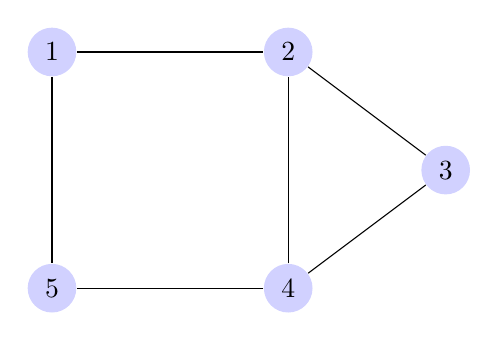
\begin{tikzpicture}
    [scale=1.0,auto=left,every node/.style={circle,fill=blue!18}]
    \node (nA) at (5,9)  {1};
    \node (nB) at (8,9)  {2};
    \node (nC) at (10,7.5) {3};
    \node (nD) at (8,6)  {4};
    \node (nE) at (5,6)  {5};
  
    \foreach \from/\to in {nA/nE,nA/nB,nB/nC,nC/nD,nD/nB,nD/nE}
      \draw (\from) -- (\to);
  \end{tikzpicture}
  \caption[Simple undirected unweighted graph]{Simple undirected unweighted graph}
  \label{fig:simple-graph}
\end{figure}

\noindent The Markov random field satisfies:

\begin{equation}
  P(u_i\ |\ \{u_j\}_{j \in V\\N}) = P(u_i\ |\ \{u_j\}_{j \in N_i}),
\end{equation}

\noindent where $N_i$ is the so called Markov blanket of node $i$.
It describes that the graph should be conditionally independent of all of the other variables given its neighbors.
A hop from one node to another can be seen as a chain of probabilities which have to occur, also called Markov chain.
The main idea behind MRF in combination with computer vision problems is to formulate the labelling problem in such a way, that each pixel has a likelihood to belong to a certain label \citep{tamassia2013handbook}.
The core problem is to find exactly one label for each pixel, which is represented as a node in a MRF.
This label represents the optimal solution to an underlying problem, in the case of stereo correspondence: the disparity of a pixel regarding a reference pixel \citep{cyganek2011introduction}.
\newline\newline\noindent Contrary to MRF, also Bayesian networks exist.
A Bayesian network is a directed graph whereby MRF is undirected.
This implies an important aspect: the direction of a certain probability to hop from one node to another.
Whereby MRF can not represent induced and non-transitive dependencies.
Two independent random variables may be connected by an edge because of possible dependencies.
Bayesian networks overcome these limitations.
\newline\newline\noindent The underlying stereo model of the Middlebury MRF library is based on the research of \citeauthor{sun2003stereo}.
They model stereo matching by three coupled MRF \citep{sun2003stereo}:
\begin{itemize}
  \item $D$ as the smooth disparity field,
  \item $L$ for representing depth-discontinuities,
  \item $O$ is a spatial binary state for handling occlusions.
\end{itemize}
\noindent Figure \ref{fig:mrf-stereo-matching} depicts the relationship between $D$, $L$ and $O$.
The conditional probability\footnote{Bayes' theorem: $P(A|B)$, a conditional probability, is the probability of event A occurring, given that event B occurs. $P(A|B) = \frac{P(B|A)P(A)}{P(B)}$ where $P(A)$ and $P(B)$ are the marginal probabilities of event $A$ and $B$. $P(B|A)$ is the probability of observing event B given that A is true.} over $D$, $L$ and $O$ given a pair of stereo images $I = {I_L,I_R}$ is defined as:
\begin{equation}
  P(D,L,O|I) = \frac{P(I|D,L,O)P(D,L,O)}{P(I)}.
\end{equation}
They then approximate inference via belief propagation over this equation.
For a deeper dive into this topic compare \citep{sun2003stereo, tamassia2013handbook, cyganek2011introduction, yedidia2003understanding, boykov2001fast, kolmogorov2006convergent, wainwright2005map}.

\begin{figure}[h!]
  \centering
  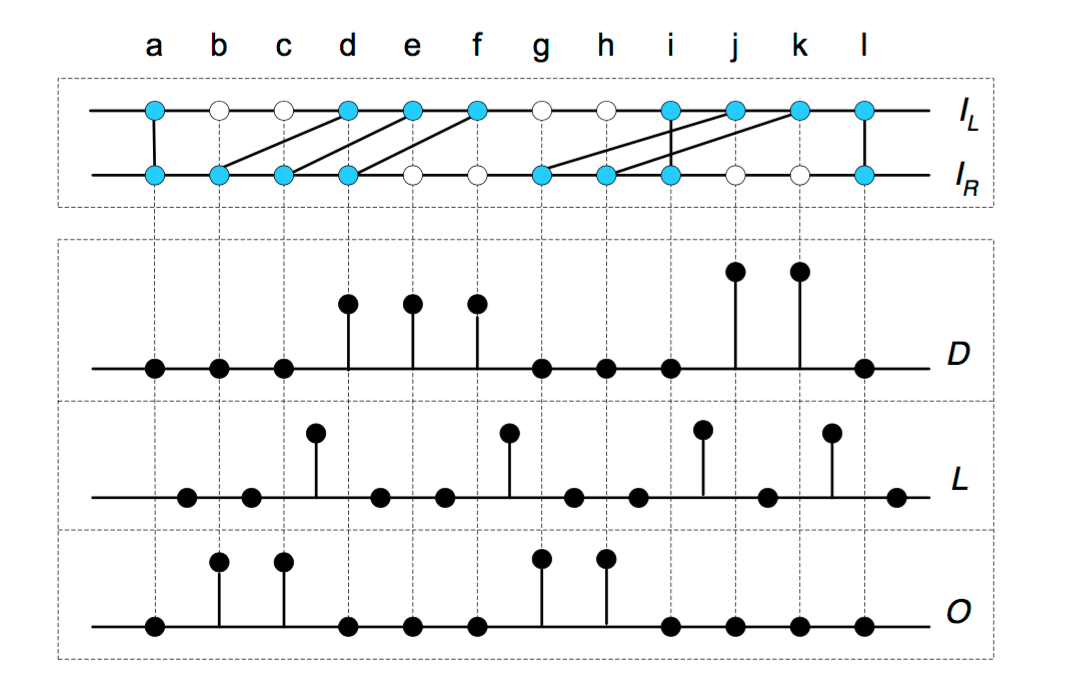
\includegraphics[width=0.9\textwidth]{src/images/mrf-stereo-matching.png}
  \caption[Stereo matching model by three coupled MRF's]{Stereo matching model by three coupled MRF's \citep{sun2003stereo}.}
  \label{fig:mrf-stereo-matching}
\end{figure}

\subsubsection{Factor graph}

\noindent As those problems are \textit{NP-hard}, several approximation algorithms exist which are outlined in the following subsections.
All of these approximation algorithms work on factor graphs.
A factor graph represents a factorized function of several variables.
Usually two types of nodes exist in factor graphs, squared and circled ones.
Circled ones represent variables of a factor and a squared one represents a factor.
Factors define the relationship between variables in the graph as they are obtained by the factorization of the function.
Such graphs are bipartite, that means that the nodes of a graph can be divided into two disjoint sets, for instance $U$ and $V$, such that every edge connects a node $U$ to one in $V$.
These factor graphs help to understand the underlying problem and to imagine the implementation of such algorithms as they are used for breaking down a problem into pieces.
\newline\newline\noindent A MRF function is factorized in partial functions and then formulated as a factor graph.
The solution to the problem represented by the factor graph is then approximated.
An important notion of factor graphs is the message which can be passed from a node to another.
So the edges represent communication channels through which messages can be passed.
One way to approximate such a factorized function is the use of message passing algorithms (also called belief propagation), which are described later on.
One exception exists: if the factor graph contains no cycles, meaning it can be represented as a tree, the solution can be computed exactly.

\subsubsection{Dynamic programming}

In general, dynamic programming means means dividing an optimization problem into smaller chunks.
These chunks get solved individually and in the end, they are connected and the optimization problem is minimized \citep{angel1972dynamic, bellman2015applied, cyganek2011introduction}.
For stereo matching this applies to the partition of a two-dimensional search problem into a series of isolated one-dimensional search problems on each pair of epipolar lines.
These problems are then solved independently.
With dynamic programming the following energy function (introduced in the foundations Chapter \ref{chap:foundations}) can be solved independently per scanline.

\begin{equation}
  E(d) = E_{data}(d) + \lambda E_{smooth}(d)
\end{equation}

\noindent Dynamic programming has two benefits, it is solvable efficiently in polynomial time and it enforces the ordering constraint (as it is solved per scanline).
But it can lead to streaking effects, meaning that the result image seems to be constructed of many independent layers.

\subsubsection{Belief propagation}

Belief propagation (BP) in general is a technique to perform inference on a probabilistic model like Bayesian networks or Markov random fields \citep{yedidia2003understanding, tappen2003comparison, cyganek2011introduction}.
As mentioned before, \citeauthor{sun2003stereo} presented a stereo model for belief propagation.
BP works with messages which are passed from one node to another.
This is the reason why BP is also known as the message-passing algorithm.
The nodes exchange information about probabilities.
In the case of stereo matching, the message contains the probability that the receiver node (a node in MRF) should hold a disparity which is consistent with all information already passed to it by a sender.
The nodes are partitioned into low- and high-confidence ones.
The messages also carry a property, the entropy.
The entropy is high when sending from low- to high-confidence nodes and vice versa (cf. \citep{yedidia2003understanding, tappen2003comparison, cyganek2011introduction}).
The nodes calculate a new state after an iteration as they know more about the other node's properties, i.e. marginal probabilities of distant and not directly connected nodes.
Also the outcome of past iterations, which yields in joint- and conditional probabilities, influences the overall state of a node.
When talking about disparity algorithms, the algorithm ends in a tree if no state is changed anymore and the exact energy can be inferred.
In an acyclic graph the algorithm finishes if the overall energy does not improve anymore.

\subsubsection{Graph cuts}

An additional method to approximate solutions to problems described by Markov random fields, graph cut algorithms can be used \citep{boykov2001fast, cyganek2011introduction}.
In general, graph cuts assume a graph $G$ with a set of nodes $N$ and connected by a set of edges $E$.
The goal is to delete enough edges so that each pixel is connected to exactly one label node.
Given a weighted graph $G$ with source $s$ and sink $t$ nodes.
The graph should be partitioned into two subsets, $S$ and $T$, where $s \in S$ and $t \in T$.
This cut with $S$ and $T$ build a cut-set $C = (S,T)$.
Basically, the goal is to find a cut which is minimum, i.e. if the size or weight of this cut is smaller than the size of any other cut.
Thus, the cut-set represents a cut such that the sum of edge weights spanning this partition is minimized.
\newline\newline\noindent In the case of computer vision, graph cuts are inspired by the combinatorial optimization methods for maximum flow \citep{cyganek2011introduction, cormen2009introduction}.
Two basic variations of the maximum flow problem exist, called $\alpha$-$\beta$-swap and $\alpha$-expansion.
Initially, three labels exist: $\alpha$, $\beta$ and $\lambda$. 
Normally, one step would be to change the label of a pixel, calculate the energy again and then infer if the change was good or not, depending on the delta.
For instance one pixel labelled with $\lambda$ would then be $\beta$.
The $\alpha$-$\beta$-swap algorithm interchanges whole areas of $\alpha$ with $\beta$ whereby areas of $\lambda$ remain unchanged.
In an $\alpha$-expansion a huge number of pixels labelled $\beta$ and $\lambda$ are changed into $\alpha$.
But in each of those methods the outcome is then measured.
In Chapter \ref{chap:foundations} the following equation was introduced:
\begin{equation}
  D = \arg\min_{d} E(d).
\end{equation}
\noindent If the outcome of such a swap or expansion is better, meaning $E(D_{after}) < E(D_{before})$, the algorithm continues.
If not, the algorithm stops.
Thus, both algorithms are expected to be stopped after the first unsuccessful run (i.e. energy increases).
The difficulty is to find the optimal swap move.
As starting point an arbitrary label is chosen.
Both is described in \citep{boykov2001fast, sinha2004graph, tappen2003comparison, ramin2004energy}.

\section{Disparity algorithms on videos}

Although stereo correspondence is a research field which has been heavily investigated for a few decades, no disparity algorithms that directly target videos yet exist.
One reason for that could be the lack of solid ground-truth data as only a few datasets has been introduced lately \citep{Butler:ECCV:2012, scharstein2014high}.
Also the computational bottleneck of dealing with multi-dimensional data can be an issue, for instance adding a new dimension to the disparity space image which reflects the relationship between multiple frames.
As a video is defined by multiple consecutive frames, every disparity algorithm for images can also be applied on videos.
The drawback of this trivial approach is the lack of taking the correlation of the frames into account.
However, novel approaches were presented by \citeauthor{khoshabeh2011spatio} \citep{khoshabeh2011spatio}, \citeauthor{lee2012local} \citep{lee2012local}, \citeauthor{davis2003spacetime} \citep{davis2003spacetime}, \citeauthor{richardt2010real} \citep{richardt2010real}, \citeauthor{hosni2012temporally} \citep{hosni2012temporally}, and are in the following section.

\subsection{Spatiotemporal consistency}

The following approaches commonly target the occurrence of noise.
On the one hand, noise can occur through estimating disparity.
The disparity maps may vary from frame-to-frame which can lead to a flickering effect over time, often perceived as disturbing \citep{khoshabeh2011spatio}.
This happens because each frame is observed separately rather than as a coherent and consecutive signal over time.
On the other hand, image or video sensors always produce little noise, although it may not be visible for humans.
As a matter of fact, stereo images from real cameras will produce kindly different images due to a variety of reasons, for instance sensor response differences or luminance \citep{khoshabeh2011spatio, cyganek2011introduction}.
Thus, they will not completely match each other which can also yield to noise in disparity maps.
Another important factor for the occurrence of noise, which has not been investigated yet, is video compression.
This idea is more described in the implementation Chapter \ref{chap:impl}.
\newline\newline\noindent \citeauthor{khoshabeh2011spatio} \citep{khoshabeh2011spatio} present a two steps approach for dealing with spatiotemporal consistency.
First, the disparity maps are computed frame-by-frame.
The computed disparity maps are treated as a space-time volume.
Then they apply a video restoration algorithms to reduce noise in this space-time volume.
This video restoration algorithm is based on the augmented Lagrangian method for total variation (TV) image restoration \citep{chan2011augmented}.
Basically, it is an algorithm for denoising images by looking at the frames before and after the current frame.
Thus, object edges and depth-discontinuity areas are preserved.
By applying this algorithm they benefit from three properties of the algorithm: variation regularization, spatial smoothness and temporal consistency, which are established at the same time.
This leads to more accurate and spatiotemporal consistent maps.
To simulate real scenery they added gaussian noise to rendered sequences, distributed as $\mathcal{N}(0,20)$\footnote{Normal (gaussian) distribution is denoted as $\mathcal{N}(\mu,\sigma^2)$, where $\mu$ is the mean and $\sigma^2$ the variance.}.
The outcome produces better results when comparing bad pixels (threshold of 1) and visually clearly better disparity maps as depict in Figure \ref{fig:spatiotemporal}.
As this approach works on computed disparity maps, current image-based disparity algorithms can thereby be easily adapted to the video domain.

\begin{figure}[h!]
  \centering
  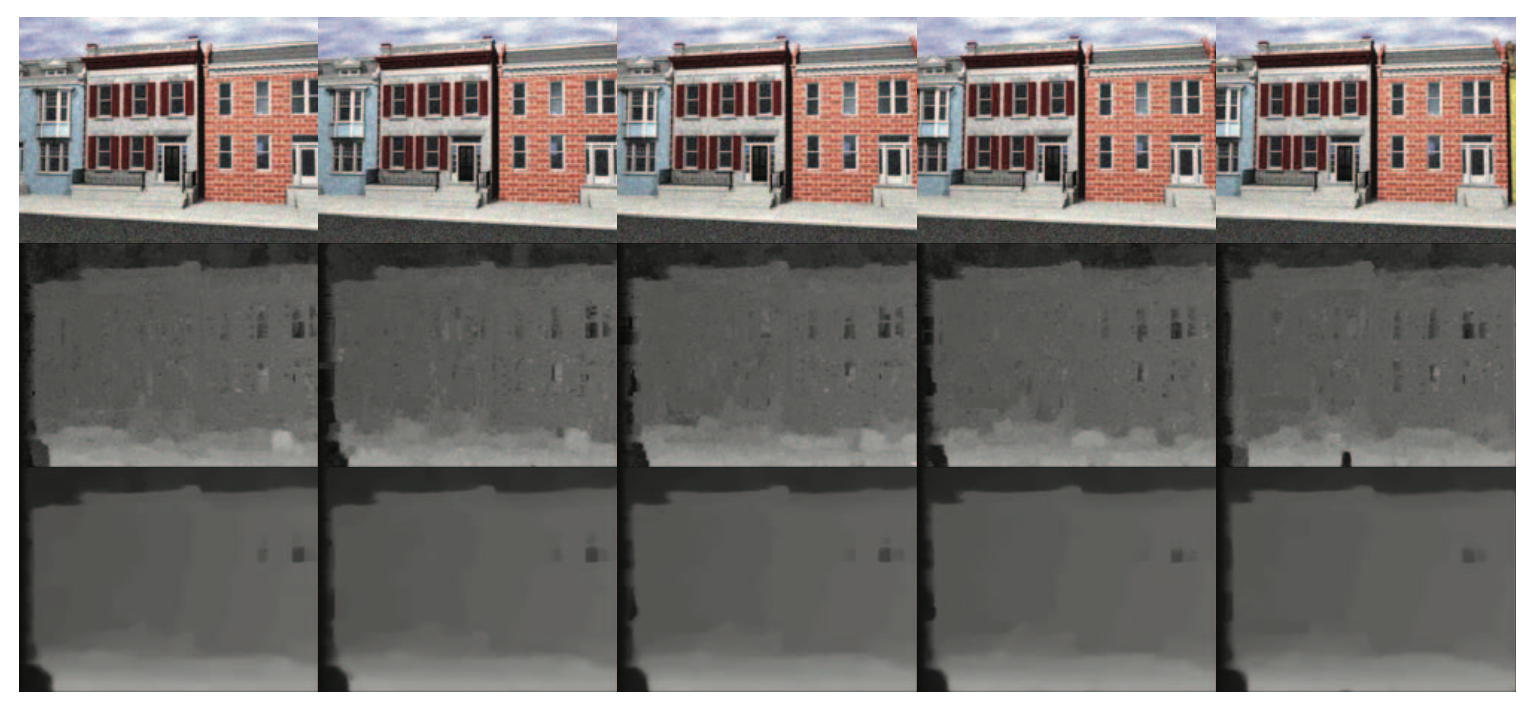
\includegraphics[width=1.0\textwidth]{src/images/spatiotemporal.png}
  \caption[Spatiotemporal disparity refinement with the augmented Lagrangian method for TV]{Spatiotemporal disparity refinement with the augmented Lagrangian method for TV \citep{khoshabeh2011spatio}. Top: Original. Middle: Disparity. Bottom: Processed.}
  \label{fig:spatiotemporal}
\end{figure}

\noindent Yet another approach regarding video disparity estimation utilizing the spatiotemporal method above is presented by \citeauthor{lee2012local} \citep{lee2012local}.
They focus on salient regions in the video.
Motion is an important factor in video processing.
Algorithms for estimating salient regions in videos exist.
Generally, moving objects lean towards a higher degree of saliency.
As typical disparity algorithms tend to have difficulties in estimating the disparity along moving edges and textureless areas, this can help to focus on especially those areas.
They utilize motion cues\footnote{Motion cues are responsible for the perception of motion.} in combination with a modified census transform\footnote{Census transform is basically an algorithm, implemented as a filter, for the classification of textures.} with a noise buffer to obtain disparity maps.
These disparity maps are more accurate and robust towards the edges of moving objects and in textureless areas.
Finally, they also apply the previously introduced method to derive a spatiotemporal consistency.
\newline\newline\noindent The work of \citeauthor{richardt2010real} \citep{richardt2010real}, \citeauthor{hosni2012temporally} \citep{hosni2012temporally} is build on the same principle, which has its origin in the basic approach of \citeauthor{davis2003spacetime} \citep{davis2003spacetime}.
They define a matching cost function with an additional property $T$ for the time axis.
A space-time cost volume is then generated by stacking the cost maps of input frames.
A simple approach could be to smooth the disparity over time by applying a box filter after the disparity map is computed.
This would imply that the disparities inside this space-time window are constant.
As a result object borders may be blurred up to obliteration and get lost in a non-static scene.
They overcome this issue by assuming that the disparity of an object is approximately constant over a small time window and applying weighted box filter.
Therefore they build a 3D filter kernel, which weights the pixels.
Pixels which belong to the same object get a high weight and pixels belonging to a different object a lower weight.
\newline\newline\noindent Tying in with this approach, \citeauthor{richardt2010real} \citep{richardt2010real} rewrote the filter as a so called dual-cross-bilateral filter.
Instead of using a custom weight model to preserve edges they utilize a bilateral filter which is a common edge-preserving smoothing technique.
The cross-bilateral filter preserves those edges while smoothing with respect to a different image.
A method for especially stereoscopic images is to use adaptive support weights for correspondence search (cf. \citep{yoon2006adaptive}).
This variant smoothes the cost space while preserving edges in both input images.
This combined filter is then named the dual-cross-bilateral (DCB) filter.
The implementation is called DBC grid.
Spatiotemporal consistency is retained with the added temporal dimension $T$.
Observing all frames as a whole is computational complex and difficult, because of multi-dimensional data, they consider 5 frames as one temporal entity.
The DBC grid with this added temporal constraint is called temportal DBC grid.
Their approach clearly visibly reduces errors as illustrated in Figure \ref{fig:dbcgrid}.
The Figure shows a selected frame of a recorded 'skydiving' stereo video \citep{richardt2010real}.
\newline\newline\noindent They present a real-time GPU-based implementation for competing with current state-of-the-art disparity algorithms regarding runtime.
At this point in time their implementation is the fastest technique in the Middlebury\footnote{\url{http://vision.middlebury.edu/stereo/eval3/}} benchmark.

\begin{figure}[h!]
  \centering
  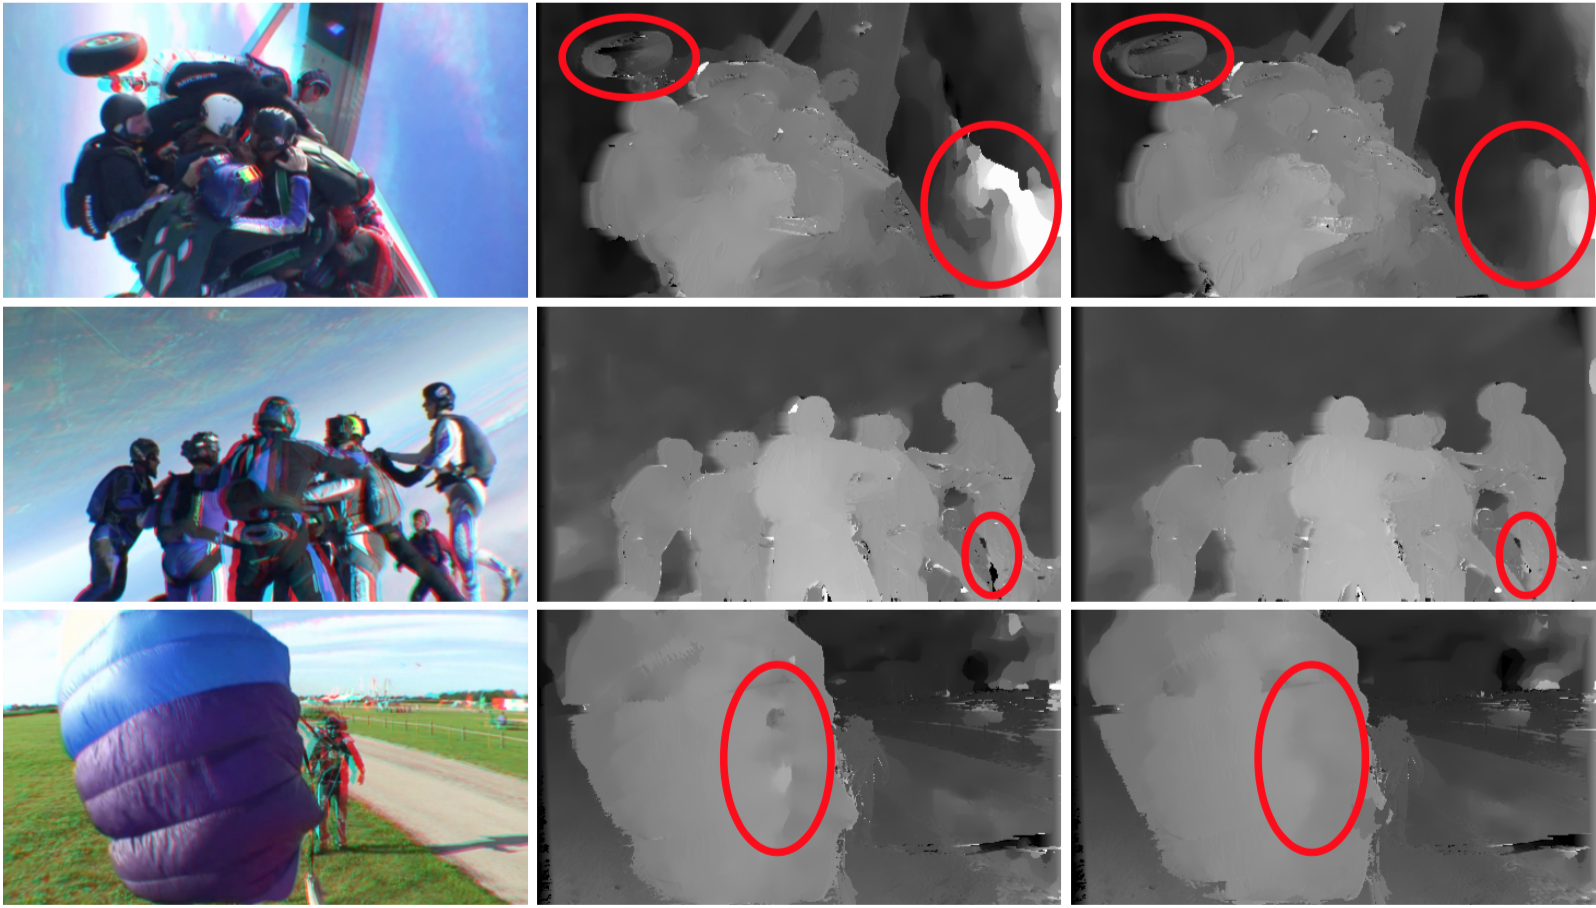
\includegraphics[width=1.0\textwidth]{src/images/dbcgrid.png}
  \caption[Disparity maps of a selected frame of the 'skydiving' stereo video]{Disparity maps of a selected frame of the 'skydiving' stereo video \citep{richardt2010real}. From left-to-right: video frame (red-cyan anaglyph), DCB Grid, Temporal DBC Grid.}
  \label{fig:dbcgrid}
\end{figure}

\subsection{Remapping the disparity range of stereoscopic videos}

\citeauthor{lang2010nonlinear} examine the problem of remapping the disparity range of stereoscopic images and videos \citep{lang2010nonlinear}.
Remapping of disparity range can be necessary for various reasons.
Humans notice the projected stereo content differently, depending on the screen size and the distance to the screen.
Another issue is negative disparity.
The fundamental underlying problem is the interplay of the human visual perception and restrictions of displays.
For instance, displaying a close object on a distant screen may result in a negative disparity and then, humans may experience the viewing as uncomfortable.
This can lead to temporary diplopia.
Those issues form a real problem in the film industry when producing 3D movies.
The disparity for the best human experience should be kept in the so called comfort zone, which is the area where eyes feel comfortable.
Too high positive disparity can lead to retina rivalry areas, which are muscular intense due to focus issues, whereas negative disparity can even result in painful retina rivalry areas.
If 3D content is optimized for a cinema screen it will look differently on a home TV screen or even a tablet device, leading to a distinct viewing experience.
This entails the need of changing the disparity after a stereoscopic movie was recorded for the adaption to the current viewing situation of the user.
For this purpose, they introduce a set of basic disparity mapping operators for the control and the retargeting of the depth of stereoscopic videos.
To actually use those operators stereoscopic warping of video streams is also presented.
Basically, those disparity mapping operators define editing operations how the disparity can be modified.
The goal is to map the disparity to a new range such that the resulting output view fulfills a stereoscopic, a temporal and a saliency constraint (cf. \citep{lang2010nonlinear}), i.e. provide consistent disparity values according to the new range.
These constraints are identical to related work on video retargeting \citep{krahenbuhl2009system}.
Stereoscopic warping is image warping with the help of the introduced disparity mapping operators.
The outcome of the paper are production-oriented rules and guidelines for editing disparity of stereoscopic content.
In a survey, user concluded that the applied techniques, i.e. stereoscopic warping with disparity mapping operators, yield in a better viewing experience due to depth structure changes without distracting visual artifacts.


\chapter{Implementation}
\label{chap:impl}

In this chapter, the thoughts made beforehand are outlined.
The following sections describe accurately the implementation, its components and the subsequent evaluation pipeline for disparity maps.
Chapter \ref{chap:related} pointed out that no real algorithm for stereoscopic video disparity exist yet.
For stereoscopic videos no evaluation engine yet exists.
Datasets with high-resolution stereo videos are rarely spread.
Source code for existing disparity algorithms are open-sourced and available for the public domain only in a few cases.
Additionally, there exist a lot of different unaligned code for evaluation and comparing disparity maps.
Thus, the decision towards a new implementation of an evaluation suite, built on top of OpenCV, was made.
Found source code of disparity algorithms was refloated and integrated.
Different masks for fine-grained evaluation were implemented as well.
An image diminisher which alters stereo images by adding noise, to simulate real scenery, or artifacts from video compression.
To round the evaluation suite up, a small web viewer to visualize the results was created.

\section{Preliminaries}

As development platform a MacBookPro was used with the following specifications: i5-4258U CPU @ 2.40GHz (dual-core), 8 GB RAM, a fast SSD.
For the later evaluation phase a desktop computer with an i5-2500k @ 3.30GHz (quad-core) was considered.
The programming part was done with Atom\footnote{\url{https://atom.io}}, a modern text editor, and CLion\footnote{\url{https://www.jetbrains.com/clion/}} from JetBrains, a cross-platform IDE especially for C++.
CMake as a cross-compiling makefile generator was utilized.
Everything except the web result viewer was implemented using C++.
As a timer saver and for reducing code duplicates OpenCV as master library was used.
The final build-chain consists of some shell scripts and CMake as makefile generator.
With CMake it was possible to cross-compile the app for Linux and use a fast server-instance from DigitalOcean\footnote{\url{https://www.digitalocean.com}} for the generation of the disparity maps and to actually evaluate those.
To not rely on different environments, a docker\footnote{\url{https://github.com/benjohnde/dockerbase-opencv}} image was created, open-sourced and used.
Docker helps developers to build, ship and run distributed applications.
A docker image serves as basis for containerized virtual environments.
Those docker containers work in a chroot\footnote{Chroot stands for "change root" and helps to change the root directory for a current process.} environment and are isolated from other processes.
It is not a complete virtualized machine as it runs on the system's kernel.
\newline\newline\noindent The final evaluation was done with python.

%todo brief description of processing chain
%todo python scripts for evaluation were used

\section{Overview}

Initially, a rapid monolithic prototype was built featuring the execution of different disparity algorithms, the creation of bitmasks and the evaluation of a given scene with different parameters.
But as more datasets were found and various bitmasks as an evaluation method were established the need for a leaner process chain arose.
Especially as disparity algorithms need some time to compute the disparity map for one frame.
Hence, as videos consist of multiple frames (in our datasets about 90 frames in mean) this is a time consuming task.
Sometimes metrics change or a new metric is established, the threshold can be adjusted.
These are the reasons for an approach towards microservices with which computed disparity maps can be evaluated repeatedly and independently.
Thus, the monolith was rewritten partitioned in smaller microservices shaping three different components:

\begin{itemize}
  \item disparity algorithm executer,
  \item mask creator,
  \item evaluation engine.
\end{itemize}

\tikzstyle{rblock} = [text width=10em, rectangle, draw, fill=blue!18, text centered, rounded corners, minimum height=4em]
\tikzstyle{cloud} = [text width=6em, ellipse, draw, fill=blue!6, text centered, rounded corners, minimum height=3.2em]
\begin{figure}[h!]
  \centering
  \begin{tikzpicture}[node distance=7em, auto]
    %input
    \node [cloud] (right) {right image};
    \node [cloud, right of=right, node distance=10em] (left) {left image};
    \node [cloud, right of=left, node distance=10em] (disp) {ground-truth};

    %computation
    \node [rblock, below of=right, xshift=2em] (exec) {(1) Algorithm executer};
    \node [rblock, below of=disp, xshift=-2em] (mask-creator) {(2) Mask creator};

    %output
    \node [cloud, below of=exec] (map) {disparity map};
    \node [cloud, below of=mask-creator] (masks) {masks};

    %evaluation
    \node [rblock, below of=left, yshift=-14em] (evaluation) {(3) Disparity evaluator};

    %final result
    \node [cloud, below of=evaluation, xshift=-5em] (csv) {csv file};
    \node [cloud, below of=evaluation, xshift=5em] (heatmaps) {heatmaps};

    %lines
    \path [line] (right) -- (exec);
    \path [line] (left) -- (exec);
    \path [line] (left) -- (mask-creator);
    \path [line] (disp) -- (mask-creator);

    \path [line] (exec) -- (map);
    \path [line] (mask-creator) -- (masks);

    \path [line] (map) -- (evaluation);
    \path [line] (masks) -- (evaluation);

    \path [line] (evaluation) -- (csv);
    \path [line] (evaluation) -- (heatmaps);
  \end{tikzpicture}
  \caption{Processing pipeline of the implementation.}
  \label{fig:impl-pipeline}
\end{figure}

%todo describe evolution
%todo describe general flow
%todo describe why it was built
%todo describe folder structure
%todo describe OpenEXR file format
%todo describe csv format of output
%todo create uml diagrams for basic implementation
%todo producing heatmaps

\noindent The figure \ref{fig:overview-uml} shows the composition and figure XXX the evaluation chain of these microservices.
The output which each one of those microservices in the chain can generate or operate on is structured in a simple folder tree:

\begin{itemize}
  \item /datasets/\{dataset\_identifier\}/\{dataset\_sequence\_identifier\}/\{appendix\}
\end{itemize}

\noindent There \{appendix\} can be either \{disparity\_maps\_computed\}, \{disparity\_maps\_smoothed\} or \{bitmasks\}.
\newline\newline\noindent The computed disparity maps are saved in a binary format since OpenCV is currently not able to use the OpenEXR file format properly (only reading is possible).
Hence for visualization they have to be normalized in the range of 0-255 or may be presented as a heat map.
The evaluation is done with simple python scripts reflecting the evaluation chain.

\begin{figure}[h!]
  \centering
  \begin{tikzpicture}

    %classes
    \umlclass[x=0,y=0]{OpenCVStereoBM}{}{}
    \umlclass[x=0,y=3,type=interface]{DisparityAlgorithm}{}{}

    \umlclass[x=5,y=0]{NaiveSmoothing}{}{}
    \umlclass[x=5,y=3,type=interface]{SmoothingAlgorithm}{}{}

    \umlclass[x=2.5,y=6]{EvalSuite}{}{- evaluateFrame()\\- evaluateFrames()}

    \umlclass[x=2.5,y=9]{Metrics}{}{}

    %connections
    \umlassoc{EvalSuite}{Metrics}

    \umluniassoc{DisparityAlgorithm}{EvalSuite}
    \umluniassoc{SmoothingAlgorithm}{EvalSuite}

    \umlimpl{OpenCVStereoBM}{DisparityAlgorithm}
    \umlimpl{NaiveSmoothing}{SmoothingAlgorithm}

  \end{tikzpicture}
  \caption{Simplified UML diagram of general architecture.}
  \label{fig:overview-uml}
\end{figure}

\begin{figure}[h!]
  \centering
  \begin{tikzpicture}

    %classes
    \umlclass[x=2,y=0]{EvalResultMetric}{}{}
    \umlclass[x=0,y=3]{FrameResult}{}{}
    \umlclass[x=4,y=3]{EvalResult}{}{}

    %connections
    \umluniassoc{EvalResultMetric}{FrameResult}
    \umluniassoc{FrameResult}{EvalResult}

    \umluniassoc{EvalResultMetric}{EvalResult}
  \end{tikzpicture}
  \caption{Simplified UML diagram of result composition for further processing.}
\end{figure}

%todo another uml diagram with the following:
%\umlclass{EvalResult}{}{}
%\umlclass{FrameResult}{}{}
%\umlclass{EvalResultMetric}{}{}

\newpage

\section{Evaluation engine for videos}

At the current point in time, no real disparity algorithm for especially videos exists yet.
As a video is defined by multiple consecutive frames, every disparity algorithm for images can be applied on videos.
The drawback of this trivial approach is the lack of taking the correlation of the frames into account.
None the less it is possible to focus on some other details, for instance:

\begin{itemize}
  \item possible outliers in the sense of frames,
  \item mean performance (error rate) of those algorithms on a complete scene,
  \item runtime variety in a sequence,
  \item analyzing the impact of noise, and
  \item trying to smooth noisy areas in the resulting disparity map with other frames.
\end{itemize}

\noindent Noise can occur through video compression.
As video sensors tend to be noisier than image sensors it also more present in stereoscopic videos, if not rendered by a computer.
As noise can be simulated and added onto the rendered video, it is investigated how noise disturb stereo matcher.
As these ideas are more explained in the implementation chapter \ref{chap:impl} the following subsection a novel approach for videos are examined.

In contrast to other implementations, input and output are clearly defined and thus different techniques can be adapted easily.
There exist combined frameworks which fulfill two tasks, disparity calculation (as the algorithm is implemented) and the final evaluation step.
This makes it harder to use the evaluation module separately from the rest.
None the less the open source community around computer vision also lacks of code for stereo matcher.
Due the diversities of algorithms and eval suites the decision was made to go for an OpenCV implementation of an eval suite for disparity algorithms.

%todo
Works basically as a wrapper. Can output statistical stuff. Basically works on disparity maps / images.

Huge mistake could be to apply the metrics on the whole disparity map from the algorithm. The output contains areas which are black (value = 0). This can be:

\begin{itemize}
  \item noise
  \item mistaken be the algorithm
  \item expected disparity
  \item non-occluded areas
\end{itemize}

\tikzstyle{block} = [rectangle, draw, fill=blue!20,
    text width=5em, text centered, rounded corners, minimum height=4em]
\tikzstyle{line} = [draw, -latex']
\tikzstyle{cloud} = [draw, ellipse,fill=red!20, node distance=4cm,
    minimum height=2em]

\begin{center}
\begin{tikzpicture}[node distance = 2cm, auto]
    \node [block] (init) {initialize eval engine with input};
    \node [cloud, left of=init] (gt) {ground-truth data};
    \node [cloud, right of=init] (ao) {algorithm output};
    \node [block, below of=init] (calc) {calculate differences};
    \node [block, below of=calc] (evaluate) {apply statistical methods};
    \node [block, below of=evaluate] (output) {output};

    \path [line] (init) -- (calc);
    \path [line] (calc) -- (evaluate);
    \path [line] (evaluate) -- (output);
    \path [line, dashed] (gt) -- (init);
    \path [line, dashed] (ao) -- (init);
\end{tikzpicture}
\end{center}

The eval engine has two modes to be queried:

\begin{itemize}
  \item via command-line which also results in a console output,
  \item with a configuration file ($config.json$) which leads to an output in a given folder for the web result viewer.
\end{itemize}

\subsection*{Preprocessing}

Different tasks are executed before the actual disparity algorithm are invoked and the evaluation takes place:

\begin{itemize}
  \item Normalization
  \item Gaussian noise
\end{itemize}

\subsection*{Postprocessing}

Postprocessing only consists of one task: normalization of the disparity map.
Some algorithms struggle with calculating a larger number than the number of disparities of $32$.
Some datasets only calculated the disparity to be in a range from $0$ to $63$.
Grayscale normally ranges from $0$ to $255$.
Thus the disparity map is normalized to range from $0$ to $63$.

Simply only disparity normalization.

\newpage

\section{Fine-grained evaluation via masks}

The evaluation would be trivial by just comparing the computed disparity map with its ground-truth companion.
This trivial comparison would be a pitfall, as the results would be erroneous due to a variety of reasons.
To give an example, occluded regions would lead to a higher error rate.
As remedy, masks are introduced to simply focus on interesting pixels.
Masks are normal matrices of the size of the input image and they reflect two states $0$ and $1$ like a bit, whereas $1$ stands for masked.
In the literature they sometimes also named bitmasks.
In this section the following masks are introduced and how they are determined:

\begin{itemize}
  \item depth-discontinuity,
  \item textured regions,
  \item occluded pixels,
  \item salient regions.
\end{itemize}

\noindent Programmatically they are represented through the OpenCV matrix class \texttt{cv::Mat} which can not work as a binary matrix and obtain just two states.
Thus, a \texttt{cv::Mat} with \texttt{CV\_8U1} is initialized, which means one color channel utilizing 8-bit unsigned for the values.
In this matrix, $255$ represents a $1$.

\subsection*{Depth-discontinuity}

Determining correspondence can fail in textureless or depth-discontinuous regions as mentioned beforehand.
Thus, it is interesting to see how disparity algorithms handle such regions.
For this purpose, a depth-discontinuity mask was implemented.
\newline\newline\noindent Depth-discontinuity is observed in a ground-truth disparity map. $gap$ and $width$ are both input parameter.
\newline\newline\noindent The image gets dilated to get the maximum disparity of a pixels neighbor.
Then, the image gets eroded for estimating the minimum disparity of pixels neighbor.
Finally, the depth-discontinuity areas are the ones with maximum - truth > gap.



"Stereo vision algorithms typically compute erroneous results in regions where there is a sudden change in the depth between objects in the scene. They are defined in [1] as regions where neighboring disparities differ by more than a certain gap, dilated by a window of a given width."
\citep{scharstein2002taxonomy, cyganek2011introduction}.

Explain:

\begin{itemize}
  \item Dilate
  \item Erode
  \item maybe show short example image (combined dilate/erode)
  \item explain how the bitmask is calculated
\end{itemize}

\subsection*{Textured regions recognition}

"Stereo vision algorithms typically compute erroneous results in regions where there is a little or no texture in the scene. They are defined in [1] as regions where the squared horizontal intensity gradient averaged over a square window of a given size is below a given threshold."
\citep{scharstein2002taxonomy, cyganek2011introduction}.

Stereo matching algorithms act on the assumption, that disparity is smooth, especially if contrast and color intensity do not change drastically.
It can be interesting to see how those algorithms treat textured and textureless regions.

Explain (shortly):

\begin{itemize}
  \item Sobel
  \item pow
  \item boxFilter
  \item how we get the bitmask
\end{itemize}

\subsection*{Discover occluded pixels}

An occluded pixel is defined as a pixel which is hidden in one of the two images, for instance an object hides it from a different angle.
In the case of stereo matching the disparity can not be calculated for such a pixel.
Thus occluded pixels have to be handled properly, as they could distort our result.
For this purpose a simple mask is introduced to indicate which pixels on the scene are visible for both cameras and which are not.

Explain and cite two papers (taxonomy of disparity algorithms).
There it is explained how everything is working.
Explain how the get the result (use algorithm).

Thus we need to take care about non-occluded areas. For this purpose we generated bitmasks (the size $w$ * $h$) for each video dataset.

"In addition to disparity maps, for stereo matching method evaluation it is interesting to have a non-occluded area mask. This mask represents in white color the pixels on the scene that are visible from both cameras and in black color the pixels that are visible from only one camera.
To obtain the non-occluded area mask, we simply cross-checked the left and right disparity maps. Pixels that are visible in both cameras will have the same value in both disparity maps, but for occluded pixels the left and right disparity value will be different.
The performance of the stereo matching algorithm on areas where pixels are occluded is one of the most important quality indicators of the algorithm, as it is very difficult to find the matching point of a pixel in one of the images if it is not visible on the other image." \citep{martull2012realistic}.

\subsection*{Saliency detection}

Another criteria for the later evaluation is how the algorithms operate on regions which are salient in a specific scene.
There exist some algorithms for saliency detection in either images or videos \citep{dittrich2013saliency, opencv_library}.
OpenCV offers two different saliency categories to be computed:
\begin{itemize}
  \item $StaticSaliency$ in images, and
  \item $MotionSaliency$ on videos.
\end{itemize}

\noindent Explain how saliency detection works, implemented via OpenCV. Otsu's algorithms, threshold and K-Means algorithm \citep{hou2007saliency}.

\section{Integration of existing algorithms}

Deciding which algorithms should be describe was not an easy task.
On the one hand, the algorithms which shall be implemented during this thesis are important and thus should be described definitely.
On the other hand, there is a huge diversity of used technologies amongst disparity algorithms.
For instance various programming languages, the decision between cpu- versus gpu-rendering, different coding styles and used libraries.
As a matter of fact, this makes it harder to implement and then evaluate every single disparity algorithm.
Thus, the algorithms from Middlebury were integrated in the evaluation suite and streamlined.
Additionally, the so called efficient large-scale stereo matcher (ELAS) was also integrated.
The parameters used for each algorithm are described in the implementation chapter.
This section is for giving an overview on these algorithms as well as their parameters for the later implementation chapter \ref{chap:impl}.

\tikzstyle{block} = [rectangle, draw, fill=blue!20,
    text width=5em, text centered, rounded corners, minimum height=4em]

\begin{figure}[h]
  \centering
  \begin{tikzpicture}[node distance = 3cm, auto]
    \node [block] (pre) {pre-processing};
    \node [block, right of=pre] (call) {call wrapper};
    \node [block, right of=call] (post) {post-processing};

    \path [line] (pre) -- (call);
    \path [line] (call) -- (post);
  \end{tikzpicture}
  \caption{Basic integration of existing algorithms}
  \label{fig:integration}
\end{figure}

This does not exist currently, so we use the Middlebury Test Suite with its algorithms for images and apply them on videos.

\begin{itemize}
	\item Consists of multiple steps
	\item Wrapper to call different algorithms
	\item normalizing of output
	\item actual eval process
\end{itemize}

Input: ImageLEFT, ExpectedLEFT, ImageRIGHT, ExpectedRIGHT
Output: a good metric for showing good/bad disparity, a few ideas.

\section{Image diminisher to simulate real use cases}

\subsection*{Gaussian noise}

randn\footnote{\url{http://docs.opencv.org/master/d2/de8/group__core__array.html\#gaeff1f61e972d133a04ce3a5f81cf6808}}

%todo finish chapter of gaussian noise

\citep{opencv_library}

As seen in the related work chapter \ref{chap:related}, some approaches use restoration algorithms in order to reduce noise which can occur.
Hence noise generation was added as a preprocessing step in order to see how noise disrupts disparity algorithms.
We use gaussian noise meaning that the noise is gaussian-distributed.

$$f\left(x\right) = a e^{- { \frac{(x-b)^2 }{ 2 c^2} } }$$

$$p_G(z) = \frac{1}{\sigma\sqrt{2\pi}} e^{ -\frac{(z-\mu)^2}{2\sigma^2} }$$

\noindent In this example, $z$ represents the grey level which is added to the image matrix later on.
$\mu$ is the mean value (= 0).
$\sigma$ is the standard deviation.
\newline\newline\noindent The $\sigma$ can be set in our evaluation suite in order to see how this distracts the image.

\pgfmathdeclarefunction{gauss}{2}{%
  \pgfmathparse{1/(#2*sqrt(2*pi))*exp(-((x-#1)^2)/(2*#2^2))}%
}

\begin{figure}[h!]
\center
\begin{tikzpicture}
\begin{axis}[every axis plot post/.append style={
  mark=none,domain=-2:3,samples=50,smooth}, % All plots: from -2:2, 50 samples, smooth, no marks
  axis x line*=bottom, % no box around the plot, only x and y axis
  axis y line*=left, % the * suppresses the arrow tips
  enlargelimits=upper] % extend the axes a bit to the right and top
  \addplot {gauss(0,0.5)};
  \addplot {gauss(1,0.75)};
\end{axis}
\end{tikzpicture}
\end{figure}

\subsection*{Video compression}

FFMPEG \citep{FFMPEG2010}.

\section{Web result viewer for evaluation suite}

For fine-tuning the algorithm's parameters as well as implementing the bitmasks it was helpful to see the visual output of both.
As the resulting bitmasks for each frame with the computed result disparity map were saved on the hard-drive for further investigations a web result viewer was created for visualizing the output.
The following features were implemented:
\begin{itemize}
  \item Starting new computations with different parameters and scene selection.
  \item Playing frame-by-frame with different speeds.
  \item Online csv-export of result.
\end{itemize}

\begin{figure}[p!]
  \centering
  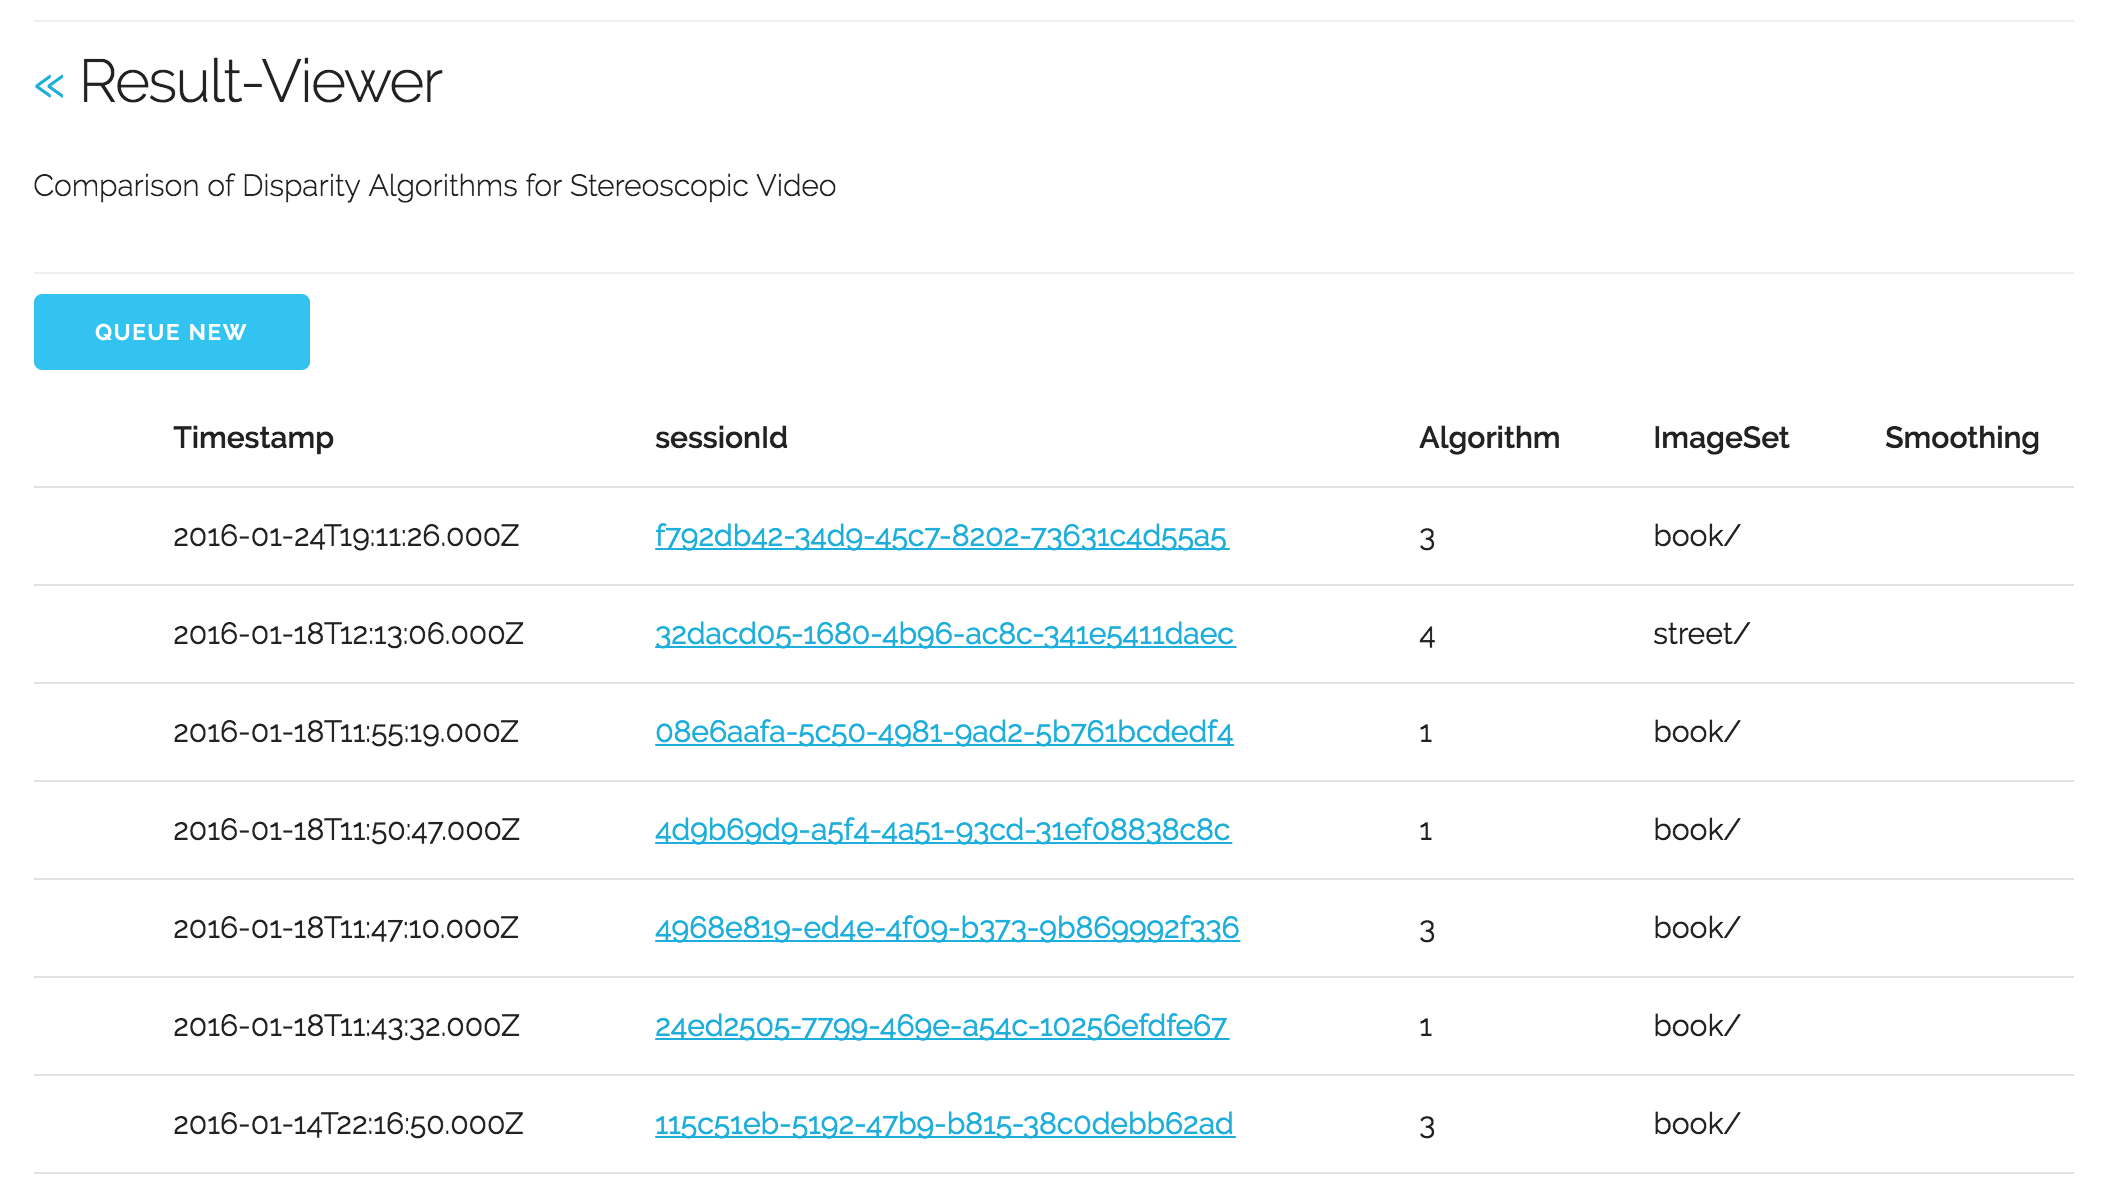
\includegraphics[angle=90,width=0.7\textwidth]{src/images/result-viewer-overview.png}
  \caption{Overview page of web result viewer.}
  \label{fig:web-overview}
\end{figure}

\begin{figure}[p!]
  \centering
  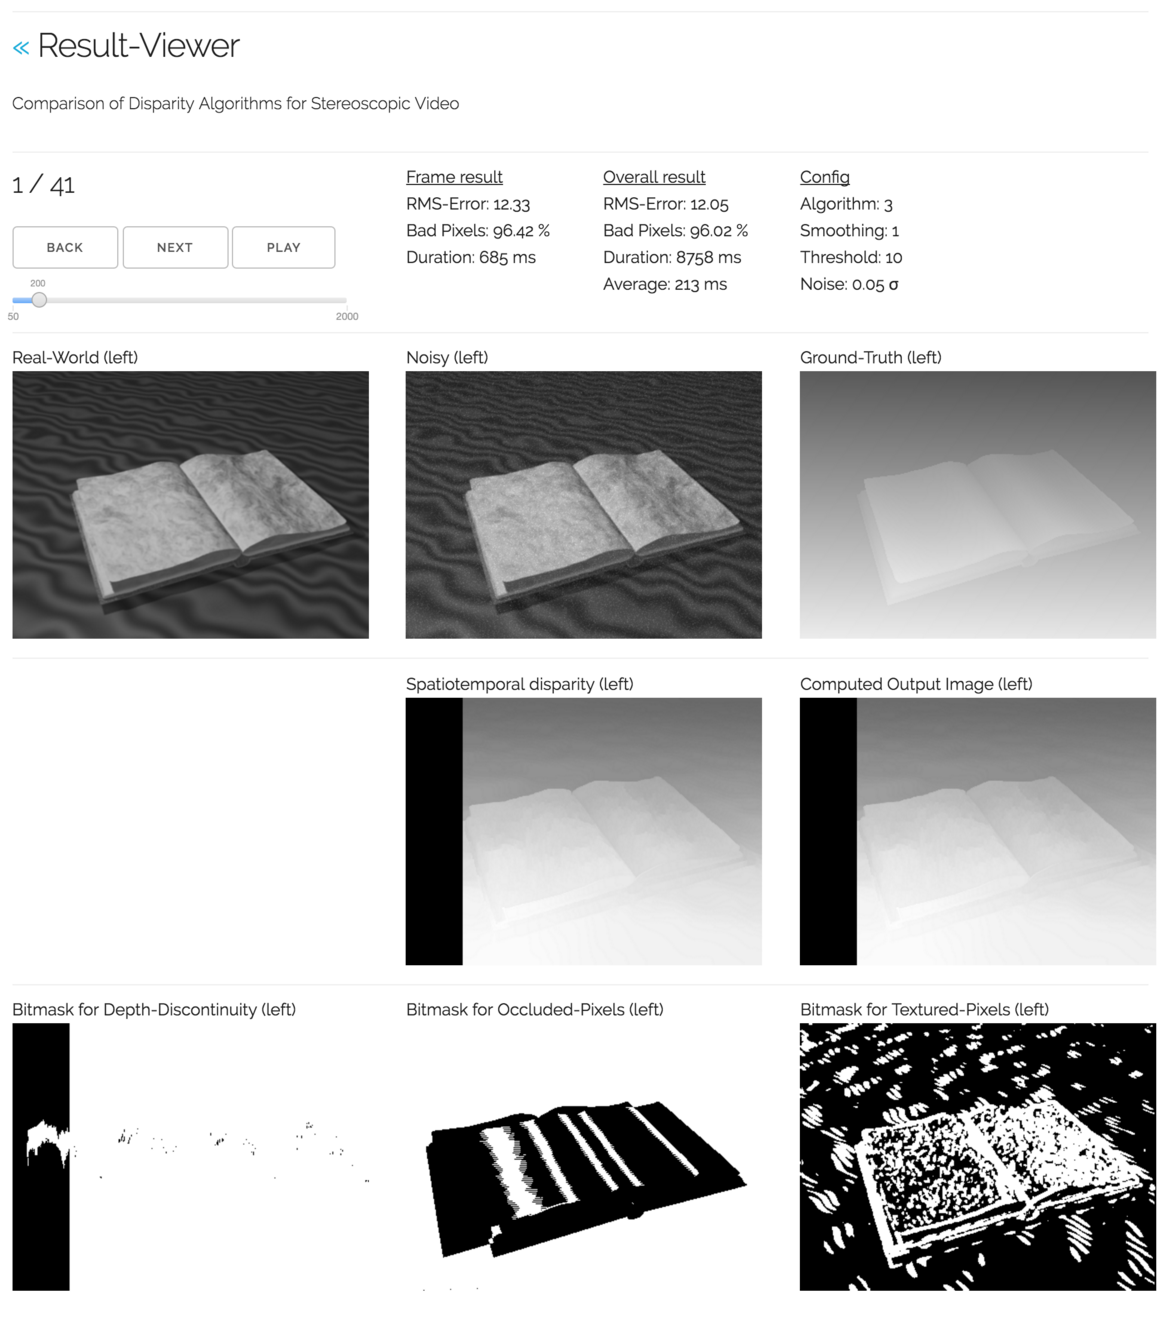
\includegraphics[angle=90,width=1.0\textwidth]{src/images/result-viewer-detail.png}
  \caption{Detail of one result in the web result viewer.}
  \label{fig:web-detail}
\end{figure}

%todo finish web result viewer section
\begin{itemize}
  \item Insert screenshot (one or two from web result viewer)
  \item Describe basic features
  \item Describe what could be done with the evaluation web suite in near future
  \item But for thesis evaluation a csv exporter was used.
\end{itemize}

\section{Discussion}

The following modules were actually implemented:

\begin{itemize}
  \item Reader for the PFM file format.
  \item Python scripts for upcoming evaluation.
  \item Shell scripts for getting the docker containers and thus the work distributed among different instances\footnote{With instances virtual machines from DigitalOcean are meant.}.
  \item Evaluation processor for
\end{itemize}


\chapter{Evaluation and results}
\label{chap:eval}

In the previous chapter, the evaluation suite and its features were presented.
This chapter is split into several sections.
At first, the datasets used for evaluation are introduced.
Afterwards, quality metrics are defined to compare disparity algorithms applied to stereoscopic videos quantitatively.
Third, the procedure of measuring the introduced metrics is described in greater detail.
Additionally, the visualization of measured results is explained.
Fourth, the results are presented and discussed.
\newline\newline\noindent Overall, the generation of all disparity maps and the process of evaluation took more than 28 days, resulting in about 50 GB of stereoscopic videos.
Accumulated, the computed disparity maps, the created masks as well as the heatmaps, allocated about 18 GB.

\section{Datasets}

A dataset basically describes a set of stereo images, which additionally contains ground-truth disparity maps.
The aim of such datasets is to provide accurate data, researchers can rely on.
This datasets can be used to evaluate the performance of computer vision algorithms, for example the disparity algorithms introduced by this thesis.
Without having such datasets it would be crucial to rate the overall quality of stereo matching algorithms.
As for today, no high-resolution stereoscopic video dataset yet exists, neither a synthetic nor a captured one.
In order to obtain ground-truth depth information, two general options are available.
On the one hand, the real-world can be sampled via area scanner, for instance a radar sensor (cf. KITTI vision benchmark suite\footnote{\url{http://www.cvlibs.net/datasets/kitti/}}).
On the other hand, a synthetic computer-animated scene is created with rendering the scene using two virtual cameras to generate disparity maps.
Of course, the former approach is more error-prone than the latter one.
The former one can lack of accuracy due to false measurements whereas the latter one provides real ground-truth information.
\newline\newline\noindent \citeauthor{kondermann2015stereo} came up with an interesting approach:
as area scanners are never 100 percent accurate, they introduced error-bars, which can range from $0-10$.
An error-bar indicates the certainty of an area scanner, that the measured disparity at a given pixel is valid \citep{kondermann2015stereo}.
As it would be a tremendous task to evaluate every existing stereoscopic dataset with every existing disparity algorithms, three different datasets to focus on in the context of this thesis were chosen.
Other datasets, which were found but not investigated are the MPI Sintel Stereo Training Data, created for optical flow evaluation \citep{Butler:ECCV:2012} and the Middlebury stereo dataset, which provides real images with ground-truth information \citep{scharstein2006middlebury}.

\subsection*{Tsukuba stereo dataset}

As reference dataset, the reworked Tsukuba Stereo Dataset was chosen \citep{martull2012realistic}.
One of the three scenes is called tsukuba to honour the popular \textit{Head and Lamp} scene and was shortly introduced in the foundations in chapter \ref{chap:foundations}.
The reference dataset is used to see if the implementation leads to similar results as in other stereo benchmarks.
This does not verify that the presented implementation is error-free but can point in the right direction.
Of course, the settings (i.e. parameters of an algorithm) depends on the input material (e.g. size of the images, noise occurrences) and on the type of scenery, for instance many regions with arbitrary surfaces (textured vs textureless).
Hence, it is possible to have good parameters for one scene and not for another.
However, in order to evaluate those algorithms, the reference dataset is used to see how the evaluation engine actually works with the same parameters on the same images.

\begin{figure}[h!]
\centering
\begin{tabular}{ccc}
\subfloat[tsukuba scene]{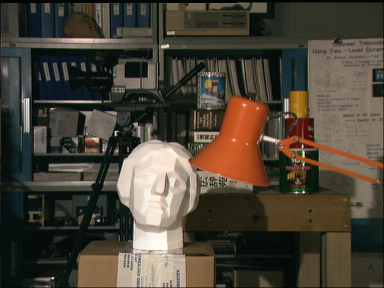
\includegraphics[width=0.3\textwidth]{src/images/tsukuba-imgL.png}} &
\subfloat[teddy scene]{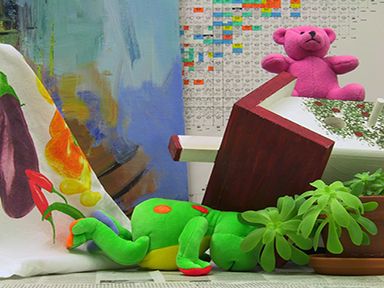
\includegraphics[width=0.3\textwidth]{src/images/teddy-imgL.png}} &
\subfloat[venus scene]{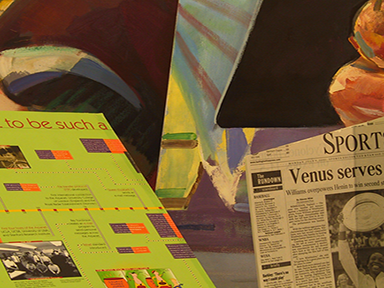
\includegraphics[width=0.3\textwidth]{src/images/venus-imgL.png}} \\
\subfloat[tsukuba disparity]{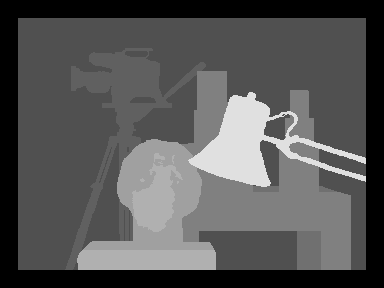
\includegraphics[width=0.3\textwidth]{src/images/tsukuba-dgt.png}} &
\subfloat[teddy disparity]{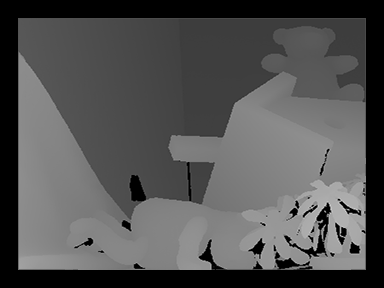
\includegraphics[width=0.3\textwidth]{src/images/teddy-dgt.png}} &
\subfloat[venus disparity]{
\includegraphics[width=0.3\textwidth]{src/images/venus-dgt.png}} \\
\end{tabular}
\caption[Tsukuba stereo dataset]{Tsukuba stereo dataset \citep{martull2012realistic}}
\label{fig:tsukuba2}
\end{figure}

\subsection*{Cambridge stereo dataset}

The second dataset from the University of Cambridge\footnote{\url{http://www.cl.cam.ac.uk/research/rainbow/projects/dcbgrid/datasets/}} is created especially for the evaluation of the DCBGrid.
This is also one of the first stereoscopic datasets targeting videos.

\begin{figure}[h!]
  \centering
  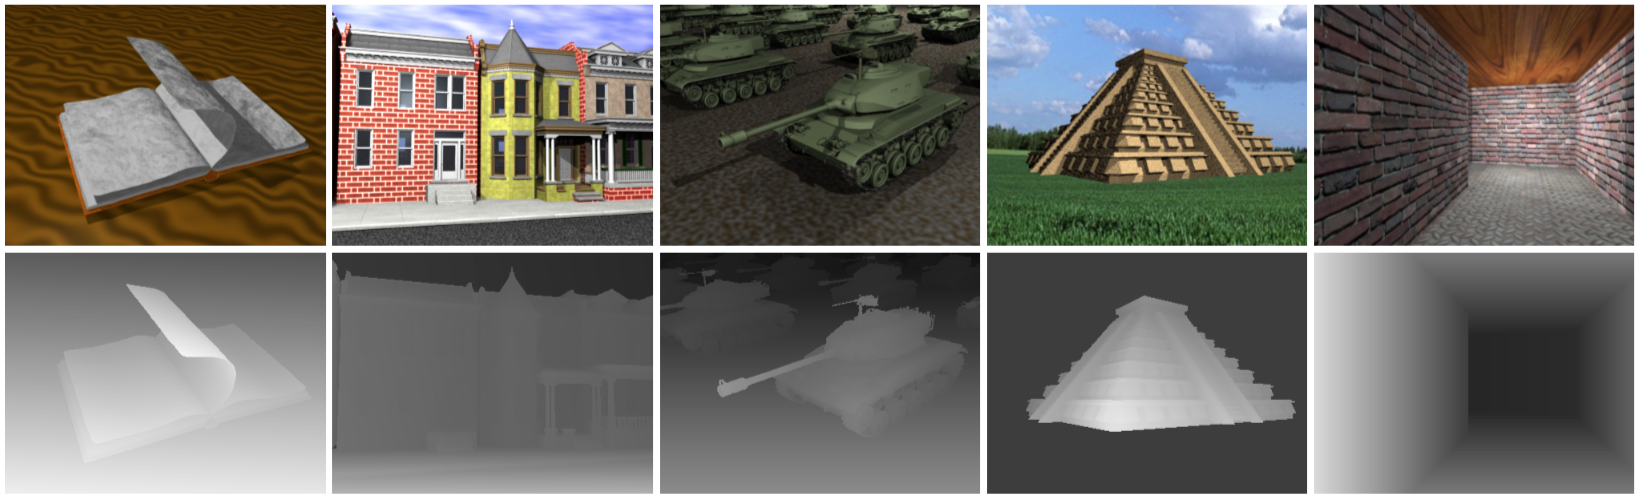
\includegraphics[width=1.0\textwidth]{src/images/dbcgrid-dataset.png}
  \caption[Cambridge stereo dataset example]{Cambridge stereo dataset example}
  \label{fig:dbcgrid-dataset}
\end{figure}

\noindent The Cambridge stereo dataset consists of five different rendered scenes at a resolution of 400 x 300 pixels, each consisting of about 100 frames \citep{richardt2010real}.
The dataset scales disparity in the range from $0$ to $64$ pixels.
The disparity maps are delivered as PNG image files, at 8 bit color depth $(0 - 255)$.
Thus, the disparity maps are loaded into a matrix and simply converted to range from $0-64$ by dividing the whole matrix through $4$.
Beforehand, the matrix is converted into $CV\_32F$, meaning that each element is represented by 32 bit floating values.

\subsection*{SVDDD - a high-resolution Stereoscopic Video Dataset with precise Depth and Disparity information}

As a third dataset, a novel, not yet analyzed dataset was chosen: the SVDDD\footnote{SVDDD stands for a high-resolution Stereoscopic Video Dataset with precise Depth and Disparity information.} dataset.
The department of Praktische Informatik IV\footnote{\url{http://ls.fmi.uni-mannheim.de/de/pi4/}} created the dataset with high-resolution video sequences containing accurate depth and disparity information for stereoscopic videos.
Figure \ref{fig:eval:svddd:intro} depicts the left image and its ground-truth disparity companion for a small selection of the SVDDD dataset.
\newline\newline\noindent The difference here is, that this dataset was not analyzed before.
Thus, it is possible that the chosen algorithms do not work properly on this dataset, which may be explained by one of the following reasons:
Either the disparity maps are not accurately calculated or the chosen algorithms doesn't apply for the constructed scenery.

\begin{figure}[h!]
\centering
\begin{tabular}{cc}
\subfloat[02-rabbit, left image]{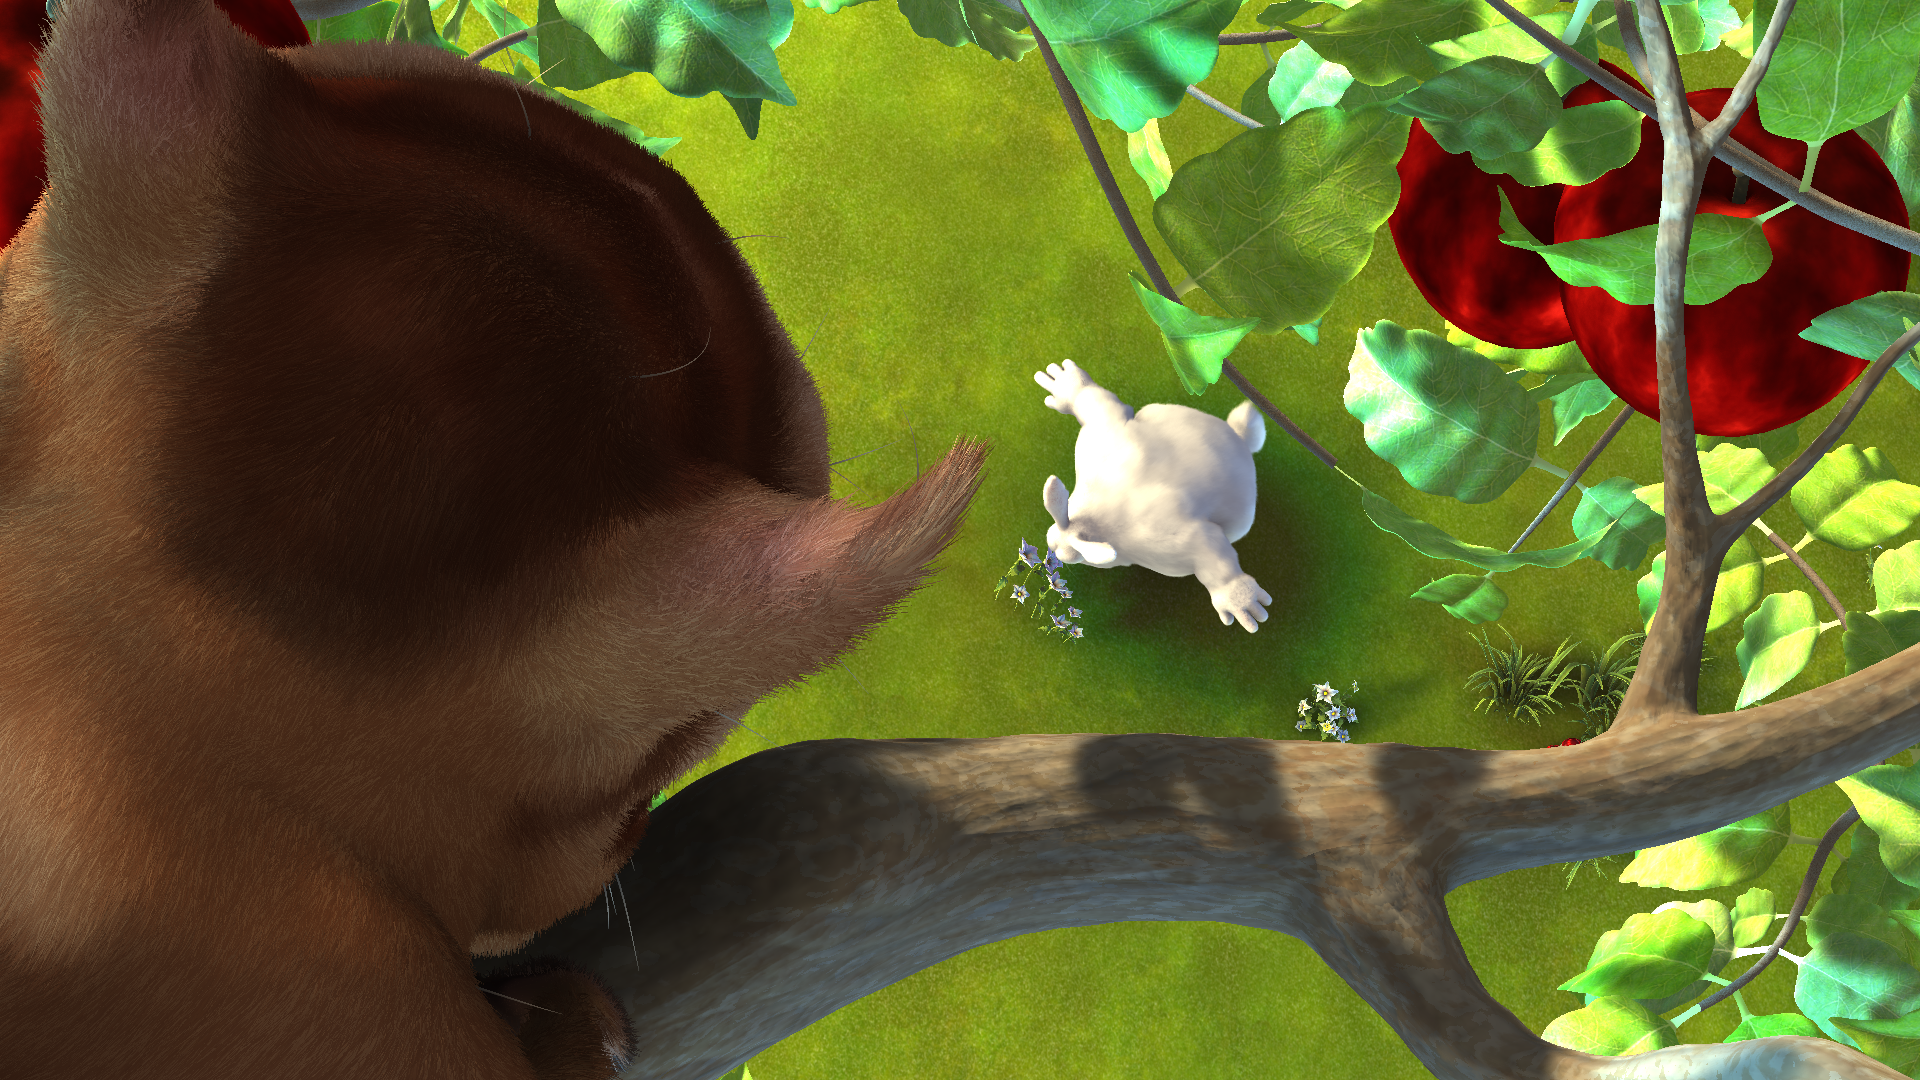
\includegraphics[width=0.45\textwidth]{src/images/evaluation/svddd/02-rabbit-left.png}} &
\subfloat[03-apple, left image]{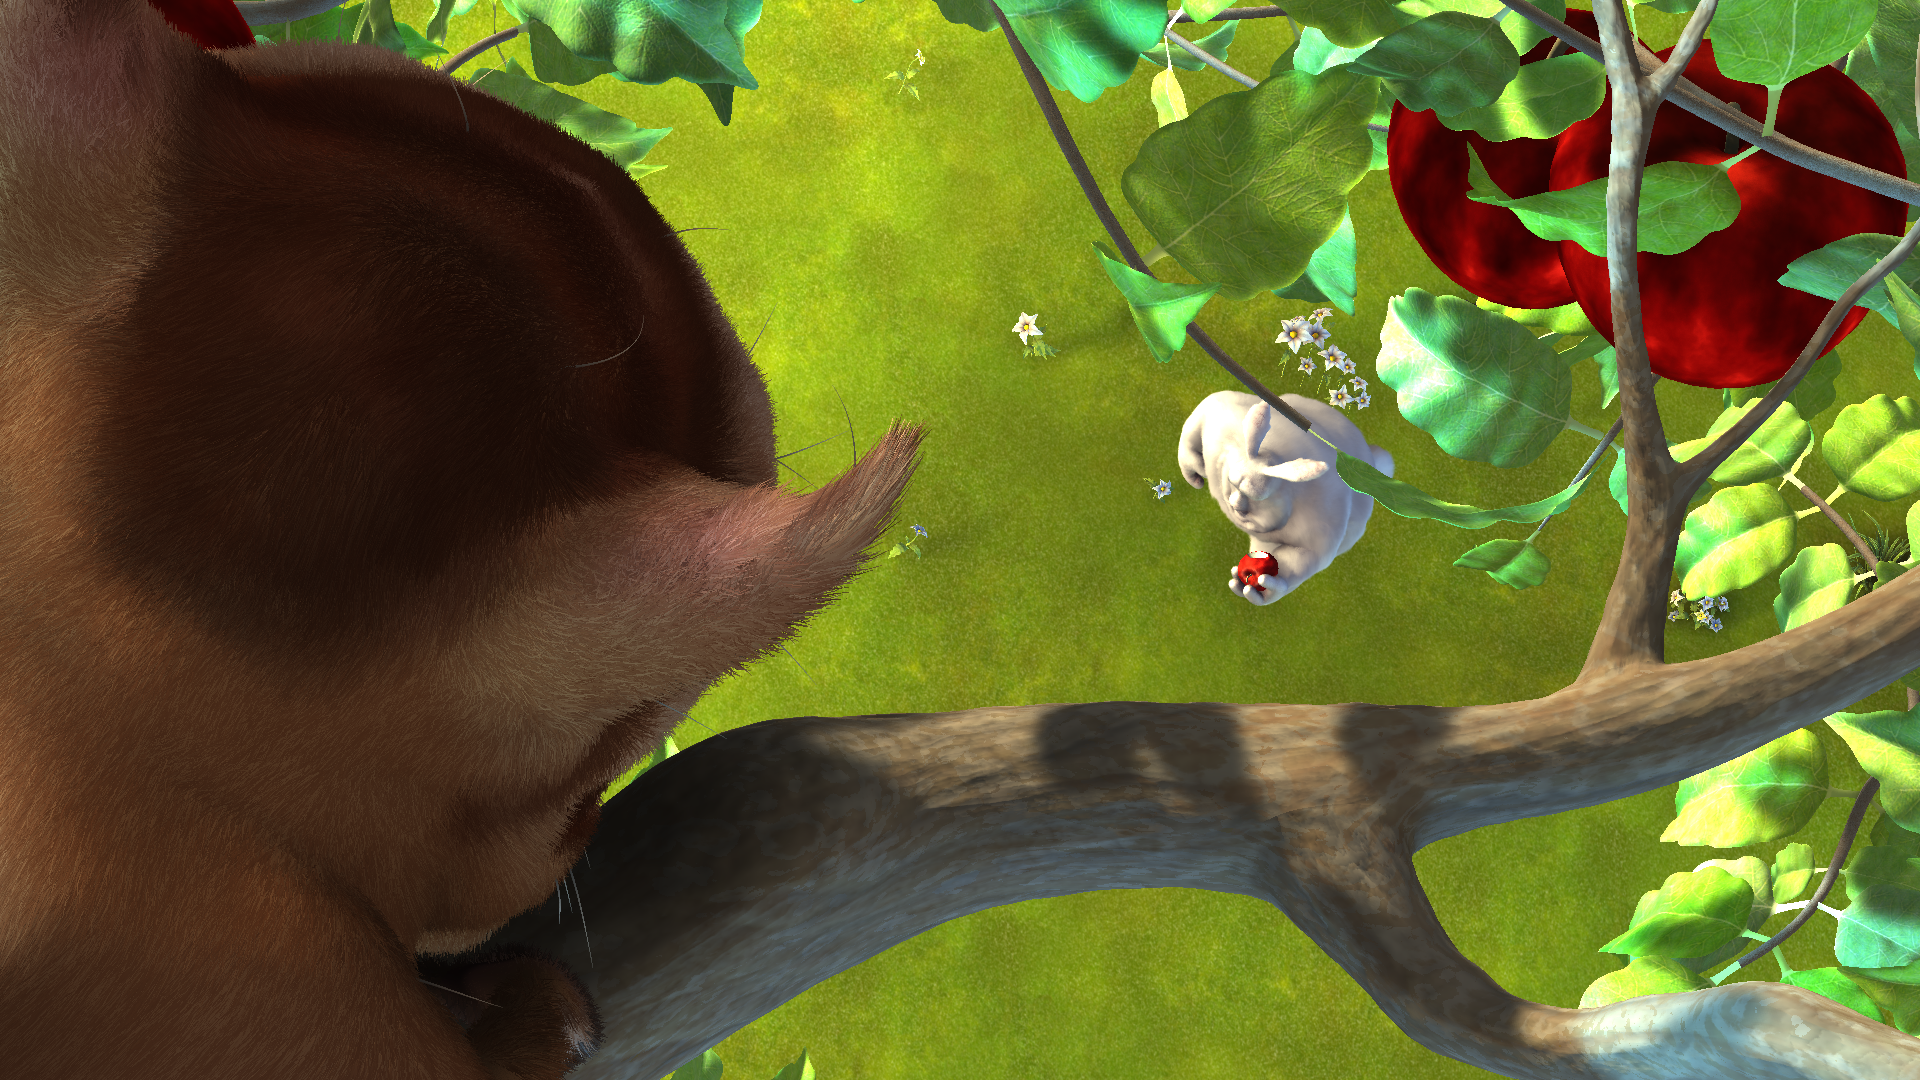
\includegraphics[width=0.45\textwidth]{src/images/evaluation/svddd/03-apple-left.png}} \\
\subfloat[02-rabbit, disparity]{
\includegraphics[width=0.45\textwidth]{src/images/evaluation/svddd/02-rabbit-disparity.png}} &
\subfloat[03-rabbit, disparity]{
\includegraphics[width=0.45\textwidth]{src/images/evaluation/svddd/03-apple-disparity.png}}
\end{tabular}
\caption{SVDDD high-resolution stereo dataset}
\label{fig:eval:svddd:intro}
\end{figure}

\noindent Focusing on the latter one, the scenes were created with Blender and utilize open-source scenes from the Big Buck Bunny project\footnote{\url{https://peach.blender.org}}.
A second camera was added to the scenes to obtain depth information.
The camera settings for each scene can be extracted from the Blender files.
With those parameters the disparity can be calculated as shown in Chapter \ref{chap:foundations}.
The scenes were also adjusted regarding the following points to extract depth-information accurately.
Rays of light as well as transparent layers were removed to retain accurate depth-information.
Such transparent layers may result in anomalous depth-information as they may bounce back the depth request while obtaining depth information from Blender.
Those transparent layers are in between the actual background of the scene, which is visible for the viewer, and the camera.
Motion and object blur were reduced as such areas can yield to defective disparity information around the blur.
Fain-grained textures like grass or fine hairs were modified.
Without modifying these elements in a scene, a stereo matching algorithm may have problems with those arbitrary textures.
The initial scenes of the Big Buck Bunny project contained randomized grass in each image, left and right side.
This also yields in the impossibility of stereo matching algorithms to determine the shift of the pixels.
\newline\newline\noindent The dataset includes 15 scenes.
Each scene consists of high resolution stereo images at 1920 x 1080 pixels with an average bitrate of 94 MBit/s.
With an approximate size of 2 MB for each frame, the size of each sequence varies between 0.4 GB and 2.7 GB.
For each frame, depth and disparity information are computed with 32-bit floating point precision and saved in OpenEXR files.
The above mentioned points apply to the first alpha version of the dataset.
During this thesis, the dataset ran through several iterations as more and more problems arose during the evaluation.
This is discussed later on.

\section{Quality metrics}

Typical quality measure instruments for comparing disparity maps against their ground-truth reference data are  \citep{cyganek2011introduction}:

\begin{itemize}
  \item percentage of bad matching pixels,
  \item root-mean-square error,
  \item parameter-free measures.
\end{itemize}

\noindent As parameter-free measures need modified disparity algorithms \citep{cyganek2011introduction}, it was not considered.

\subsection*{Percentage of bad matching pixels}

Percentage of bad matching pixels (PBMP) is usually used in comparing the performance of stereo matching algorithms.

\begin{equation}
  \operatorname{PBMP}=\frac{1}{n} \sum_{x,y=0}^{}(|d_a(x,y) - d_e(x,y)| > \delta_t)
\end{equation}

\noindent $d_a$ stands for the actual disparity whereas $d_e$ symbolizes the expected one.
The threshold, denoted with $\delta_t$, can be adjusted and as result, the percentage of outlier pixels, which differ by more than $\delta_t$, is estimated.

\subsection*{Root-mean-squared error}

The mean squared error (MSE) as well as the root mean squared error (RMSE) are both the most popular metrics in image and video processing \citep{cyganek2011introduction, benoit2008quality, scharstein2002taxonomy}.
MSE measures the mean of the squared differences between the intensities of pixels in two pictures at the same position.
In conclusion, the average difference per pixel is then the root of the squared error.

\begin{equation}
  \operatorname{RMS-Error}=\sqrt{\frac{1}{n} \sum_{x,y=0}^{}(d_a(x,y) - d_e(x,y))^2}
\end{equation}

\noindent It represents the sample standard deviation of the differences between predicted values and observed values.
Here $d_a(x,y)$ is the actual disparity value for given $x$ and $y$.
$d_e(x,y)$ is our expected disparity value from our ground-truth data.
Hence the RMSE is the difference between values on average.

\section{Measurement}

This chapter describes and summarizes the evaluation process.
All disparity maps were created on a desktop computer with an i5-2500k @ 3.30GHz (quad-core).
First, the idea of a distributed calculation arose, as described in Chapter \ref{chap:impl}.
As this would lack the comparison of runtime, only the desktop computer was used.
\newline\newline\noindent The whole evaluation was proceeded in the following manner:
Python scripts manage the chained execution of all components.
Disparity maps are computed for each frame in a sequence, for each sequence in a dataset, and for each dataset.
The Cambridge dataset contains five sequences with each 100 frames.
In total, 13 algorithms were executed.
This results in a total of $6.000$ disparity maps.
\newline\newline\noindent In addition, this dataset was duplicated for observing interferences on disparity algorithms.
For analyzing the impact of noise, additive gaussian noise with a normal distribution of $\mathcal{N}(\mu,\sigma^2)$ was added.
For $\sigma$, $10, 20, 30$ were chosen as parameter.
Lower values had no noteworthy impact on a few sample disparity maps computations and were also not visually exhibited.
Higher values were measured by \citeauthor{richardt2010real} \citep{richardt2010real}, but are clearly disturbing the whole image.
As additive gaussian noise should simulate a more real scenery instead of synthetic rendered videos, higher values were not considered.
\newline\newline\noindent Due to bandwidth limitations, raw (lossless) high resolution videos are not transmitted without additional compression.
That said, H.265, which was introduced in Chapter \ref{chap:impl}, was chosen as current state of the art video compression codec.
For analyzing the resulting inteferrence on disparity algorithms, video compression artifacts were added by converting the images to a video, applying the codec and unwrapping the video into images.
As parameter, the constant rate factor (CRF) has been adjusted.
The default parameter value is $28$.
As $0$ means lossless video compression, it was tested with a few sample disparity map computations.
$0$ had no impact and was not considered for the evaluation.
$51$ was not considered as well, as this totally disturbs the image visually, even if there is no motion between two consecutive frames.
$14, 28, 40$ were chosen as final values to have a feasible amount of different values and with an equal distribution in the available parameter range.
\newline\newline\noindent Taking those combinations into account yields to an amount of disparity maps to be computed of $48.000$.
After the disparity maps were computed, other Python scripts were written and executed for the aggregation of the results.
As the results are for each image in a sequence from a dataset and also focusing on one algorithm, they have to be aggregated and written in summarized CSV files.
The simple stereo matcher was treated as an exception.
The reason for this is simple: all the scripts were written with the intent of calculating single independent disparity maps.
As the simple stereo matcher features spatiotemporal consistency, scripts focusing especially on the execution and aggregation of this matcher were written as well.

\subsection*{Parameter tuning}

The observed parameters regarding noise and video compression were described before.
In addition, most of the available parameters were described accurately in Chapter \ref{chap:impl}.
Adjusting and quantifying also the parameters of each algorithm would be a formidable task.
Thus, only the maximum disparity was adjusted according to the dataset.
All the other variables were left as default and moreover, some algorithms have no parameter but the maximum disparity to adjust.

\subsection*{Visualization}

As it may be hard to identify fine-grained changes in grayscale images and also the human eye tends to be more sensitive to observe color changes, heatmaps are used to visualize the results.
For visualization, the heatmaps are created with the OpenCV autumn color scheme.
The color-scale of this theme is depict in Figure \ref{fig:colorscale}.

\begin{figure}[h!]
  \centering
  
\includegraphics[width=0.6\textwidth]{src/images/colorscale.png}
  \caption[OpenCV autumn color scale]{OpenCV autumn color scale\protect\footnotemark}
  \label{fig:colorscale}
\end{figure}
\footnotetext{Source (accessed 04/2016): \url{http://docs.opencv.org/3.1.0/d3/d50/group__imgproc__colormap.html}.}

\noindent Outliers are marked with three different purple color steps in the heatmaps.
The darker the purple color is, the more hard the error was.
The light blue means $1px$ threshold was exceeded, the color in-between the light blue and the dark purple denotes $2px$ threshold was exceeded and the very dark purple reflects $4px$ threshold was exceeded.
The border is excluded from the evaluation (cf. Chapter \ref{chap:foundations}) and marked black.
Brighter color means more heat and marks nearer pixels.
An example shot can be seen in Figure \ref{fig:example-heatmap}.
\newline\newline\noindent The maximum disparity in this example shot was $64$.
This means that due to the baseline separation of the cameras, and the resulting shift of the pixels, some pixels can not be calculated as they have no counterpart.
This was excluded from the evaluation.
Also, as the area-based disparity algorithms work with a window size and have a small step from the top and the bottom, this was excluded as well.
Both is represented with a border mask, which was applied to all evaluation steps beforehand.
This can also be seen in Figure \ref{fig:example-heatmap}.
This guarantees a streamlined and balanced evaluation.

\begin{figure}[h!]
\centering
\begin{tabular}{cc}
\subfloat[outliers heatmap]{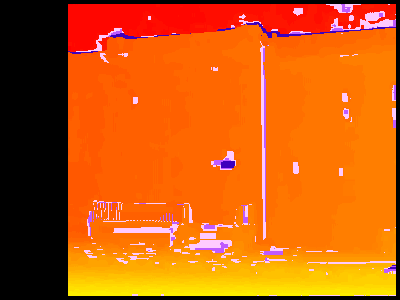
\includegraphics[width=0.45\textwidth]{src/images/evaluation/street-example-heatmap-outliers.png}} &
\subfloat[ground-truth heatmap]{
\includegraphics[width=0.45\textwidth]{src/images/evaluation/street-example-heatmap.png}}
\end{tabular}
\caption[Example heatmaps]{Example heatmaps for outliers heatmap and disparity ground-truth.}
\label{fig:example-heatmap}
\end{figure}

\subsection*{Applying disparity algorithms on videos}

As said in the implementation Chapter \ref{chap:impl}, disparity algorithms for image can be applied to videos.
Although the frames of a video can be seen as independent pieces, different anomalies can be further investigated while analyzing videos:

\begin{itemize}
  \item outliers in the form of a single frames which differs too much from the others,
  \item impact of additive Gaussian noise to simulate real scenery,
  \item impact of disturbing effects like artifacts from video compression,
  \item the benefit from creating a naive spatiotemporal context.
\end{itemize}

\noindent The following sections present only the highlights of the results as it is an tremendous amount of data, which were computed during the evaluation.

\section{Results}

The highlights are illustrated as the amount of information, which were obtained during the measurement is huge.
The following Table \ref{tab:identifier1} contains the identifier which are used throughout the upcoming subsections.
Algorithm (10) OpenCV - simple BM utilizes the same implementation as (2) OpenCV - BM but without performing a left-to-right consistency check and WLS filtering, as described in Chapter \ref{chap:impl}.
The following subsections are rationed in the results against the reference dataset, the general performance of the Cambridge dataset as well as the impact of interferences like noise and video compression.
Afterwards, the runtime and the SVDDD dataset are outlined.
As of now, the spatiotemporal approach with unweighted matching cost is denoted as \textit{SNSM - STU} whereas the weighted spatiotemporal approach is denoted as \textit{SNSM - STW}.

\begin{table}[h!]
\centering
\begin{tabular}{ll}
  \hline
  \textbf{Id} & \textbf{Sequence} \\ \hline \hline
  1 & book \\
  2 & street \\
  3 & tank \\
  4 & temple \\
  5 & tunnel \\
  & \\
  & \\
  & \\
  & \\
  & \\
  & \\
  & \\
  & \\
  \hline
\end{tabular}
\quad
\begin{tabular}{ll}
  \hline
  \textbf{Id} & \textbf{Algorithm} \\ \hline \hline
  1 & OpenCV - SGBM \\
  2 & OpenCV - BM \\
  3 & ELAS \\
  4 & MRF - ICM \\
  5 & MRF - GC Expansion \\
  6 & MRF - GC Swap \\
  7 & MRF - BP TRWS \\
  8 & MRF - BP BPS \\
  9 & MRF - BP BPM \\
  10 & OpenCV - Simple BM \\
  11 & SNSM \\
  12 & SNSM - STU \\
  13 & SNSM - STW \\
  \hline
\end{tabular}
\footnotetext{Simple stereo matcher with respecting spatiotemporal context, unweighted.}
\footnotetext{Simple stereo matcher with respecting spatiotemporal context, weighted.}
\caption{Identifier for results}
\label{tab:identifier1}
\end{table}

\noindent The general procedure is to describe the high level results of algorithms operate on a whole sequence with PBMP$_{1px}$ utilizing the non-occluded mask.
As the focus is on PBMP$_{1px}$, lower results are better.
The cell of the best result in each row is marked with green background color, the worst with red.
Then, the other masks are outlined in greater detail.
Afterwards, particular outliers regarding the whole sequence are discussed.
The same procedure is then applied to impact of noise and impact of video compression.

\subsection{Against reference dataset}

As reference scene the \textit{Head and lamp} scene of the Tsukuba dataset was chosen.
For evaluating against the reference dataset, all presented disparity algorithms computed disparity maps.
These disparity maps are then compared in combination with different masks.
The result can be seen in Table \ref{tab:eval:snsm:tsukuba} and the SNSM is depicted in Figure \ref{fig:eval:snsm:tsukuba}.
Compared with the Middlebury stereo benchmark\footnote{\url{http://vision.middlebury.edu/stereo/eval/}}, similar results could be achieved.
\newline\newline\noindent The SNSM utilizes SAD as matching cost function and does not further disparity refinement.
The results from SNSM with a threshold of $1$ and a block size of $9$ are PBMP$_{all,1px}$ = 11.51\% and RMSE$_{all} = 1.78px$.
According to the Middlebury stereo benchmark, the other SAD implementation (SAD-IGMCT) \citep{ambrosch2010accurate} achieved with a threshold of $1$: PBMP$_{all,1px}$ = 7.14\%.
The difference may come from smoothing, which SAD-IGMCT included as a disparity refinement step, which is visible while looking at their outcome.
The other results are similar to the results in the Middlebury stereo benchmark.

\begin{table}[h!]
\centering
\scalebox{0.95}{
\begin{tabular}{l|rrrr}
  & RMSE$_{all}$ & PBMP$_{all,1px}$ & PBMP$_{all,2px}$ & PBMP$_{disc,2px}$ \\ \hline
(1) OpenCV - SGBM & 1.49px & 7.00\% & 4.73\% & \cellcolor{green!50}11.99\% \\
(2) OpenCV - BM & 1.45px & 10.27\% & 5.92\% & 12.40\% \\
(3) ELAS & \cellcolor{green!50}1.23px & 7.07\% & \cellcolor{green!50}4.42\% & 12.08\% \\
(4) MRF - ICM & 5.02px & 22.32\% & 18.83\% & 19.72\% \\
(5) MRF - GC Expansion & 2.56px & 5.59\% & 4.74\% & 12.86\% \\
(6) MRF - GC Swap & 2.79px & 5.55\% & 4.70\% & 12.74\% \\
(7) MRF - BP TRWS & 2.48px & 5.41\% & 4.54\% & 12.32\% \\
(8) MRF - BP BPS & 2.64px & 9.49\% & 9.07\% & 16.27\% \\
(9) MRF - BP BPM & 2.55px & \cellcolor{green!50}5.34\% & 4.97\% & 12.99\% \\
(10) OpenCV - Simple BM & \cellcolor{red!50}6.10px & \cellcolor{red!50}28.27\% & \cellcolor{red!50}26.42\% & \cellcolor{red!50}28.99\% \\
(11) SNSM & 1.78px & 11.51\% & 9.85\% & 18.97\% \\
SAD-IGMCT & - & 7.14\% & 5.80\% & 18.90\% \\ \hline
\end{tabular}
}
\caption[Result table for reference dataset]{Result table for reference dataset}
\label{tab:eval:snsm:tsukuba}
\end{table}

\noindent Some deviations like SAD-IGMCT to SNSM regarding all pixels and a threshold of $2$ are huge but can be explained with disparity refinement steps which the SNSM does not perform.
The best result is achieved with a variant of a global method, belief propagation and yields to 4.97\% of bad matching pixels regarding all pixels and applying a threshold of $2$.
ELAS performs pretty good but struggles with a very accurate disparity map while comparing the results for PBMP$_{all,1px}$.
The simple block matching algorithm of OpenCV (10) is the same as (2), but without the disparity refinement step and a left-right-consistency check.
This may explains the very bad results.
Surprisingly, the global methods do not outperform the local methods by far.

\begin{figure}[h!]
\centering
\begin{tabular}{cc}
\subfloat[ground-truth heatmap]{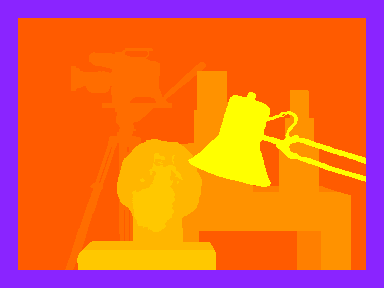
\includegraphics[width=0.45\textwidth]{src/images/evaluation/snsm-tsukuba-ground-truth.png}} &
\subfloat[computed disparity-map]{
\includegraphics[width=0.45\textwidth]{src/images/evaluation/snsm-tsukuba-disparity-map.png}} \\
\subfloat[outliers in SNSM]{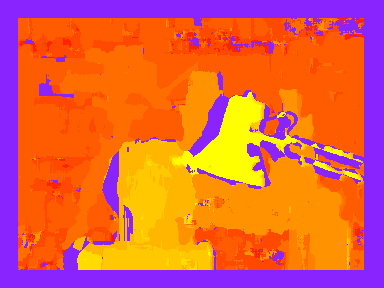
\includegraphics[width=0.45\textwidth]{src/images/evaluation/snsm-tsukuba-outliers.png}} &
\subfloat[outliers in SAD-IGMCT]{
\includegraphics[width=0.45\textwidth]{src/images/evaluation/snsm-tsukuba-outliers-igmct.png}}
\end{tabular}
\caption{SNSM heatmaps for Tsukuba scene}
\label{fig:eval:snsm:tsukuba}
\end{figure}

\noindent In the beforehand mentioned Figure \ref{fig:eval:snsm:tsukuba}, SNSM struggles with the disparity constraints as they are not forced programmatically.
For each point $(x,y)$ the disparity is calculated individually.
This leads to a more noisy disparity map than for instance the disparity map of SAD-IGMCT, which respects the disparity constraints, takes the left-right-consistency into account and performs a disparity refinement step.
But it also shows that by implementing a simple stereo matcher with just the SAD as matching cost measurement step reasonable results can be achieved.
The semi-global stereo matcher implementation of OpenCV achieved the best result in PBMP$_{disc,2px}$, which focuses on the disparity estimation near depth-discontinuities at object borders.

\subsection{General performance}

From a theoretical perspective, the assumption is that the algorithms struggle with depth-discontinuity regions and arbitrary surfaces, i.e. textureless regions.
Also, global methods should perform slightly better than local methods.
Salient regions may a bit more random as they take the spectrum of the image into account and not the nature composition of pixel groups like textures.
As it would be a tremendous task to deliver all possible plots, only the highlights were included.
\newline\newline\noindent The following Tables \ref{fig:eval:general:performance1} and \ref{fig:eval:general:performance2} contain the general performance with the focus on PBMP$_{noc,1px}$.

\begin{table}[h!]
\centering
\scalebox{0.9}{
\begin{tabular}{c|rrrrrrrrr}
  & 1 & 2 & 3 & 4 & 5 & 6 & 7 & 8 & 9 \\ \hline
1 & 16.60\% & \cellcolor{red!50}30.98\% & 7.31\% & 19.55\% & 8.30\% & 8.74\% & 8.32\% & 24.35\% & \cellcolor{green!50}6.93\% \\
2 & \cellcolor{green!50}6.88\% & \cellcolor{red!50}13.90\% & 7.18\% & 30.75\% & 10.91\% & 11.19\% & 10.90\% & 13.10\% & 8.32\% \\
3 & 9.54\% & \cellcolor{red!50}28.14\% & 3.99\% & 11.18\% & 4.17\% & 4.25\% & 4.10\% & 6.31\% & \cellcolor{green!50}3.35\% \\
4 & 13.98\% & 18.86\% & 9.90\% & \cellcolor{red!50}23.53\% & 8.01\% & 10.47\% & \cellcolor{green!50}7.75\% & 10.20\% & 11.65\% \\
5 & 5.96\% & \cellcolor{red!50}16.13\% & \cellcolor{green!50}0.19\% & 1.37\% & 3.41\% & 3.34\% & 3.42\% & 5.68\% & 0.62\% \\ \hline
$\varnothing$ & 10,59\% & \cellcolor{red!50}21,60\% & \cellcolor{green!50}5,71\% & 17,28\% & 6,96\% & 7,60\% & 6,90\% & 11,93\% & 6,17\% 
\end{tabular}
}
\caption[Result table for general performance]{Result table for general performance, focusing on PBMP$_{noc,1px}$}
\label{fig:eval:general:performance1}
\end{table}

\noindent Focusing on the general performance of all but SNSM, ELAS outperforms in mean of all sequences the other global and local methods.
The worst result is achieved with the OpenCV block matching implementation.
It is also impressive that ELAS also outperforms traditional global methods, like graph cuts and belief propagation.
None the less, it has to be mentioned, that the performance of global methods may vary intensely depending on the formulation of the underlying energy function \citep{cyganek2011introduction, szeliski2008comparative, scharstein2006middlebury}.

\begin{table}[h!]
\centering
\scalebox{0.95}{
\begin{tabular}{c|rrrr}
  & 10 & 11 & 12 & 13 \\ \hline
1 & \cellcolor{red!50}32.61\% & \cellcolor{green!50}8.72\% & 10.07\% & 9.65\% \\
2 & \cellcolor{red!50}25.64\% & 11.79\% & \cellcolor{green!50}8.76\% & 8.90\% \\
3 & \cellcolor{red!50}13.26\% & \cellcolor{green!50}6.08\% & 8.71\% & 7.29\% \\
4 & \cellcolor{red!50}38.96\% & 12.98\% & \cellcolor{green!50}11.15\% & 11.26\% \\
5 & \cellcolor{red!50}8.60\% & \cellcolor{green!50}0.93\% & 4.54\% & 2.15\% \\ \hline
$\varnothing$ & \cellcolor{red!50}23,81\% & 8,10\% & 8,66\% & \cellcolor{green!50}7,85\% 
\end{tabular}
}
\caption[Result table for general performance]{Result table for general performance, focusing on PBMP$_{noc,1px}$}
\label{fig:eval:general:performance2}
\end{table}

\noindent It is interesting to see, that the simplest variant of the block matching implementation in OpenCV is outperformed by just a SAD matching cost implementation, the SNSM.
Also, the best results are achieved with the weighted spatiotemporal approach, although the approach was not superior in at least one sequence, but overall.

\subsubsection{Depth-discontinuity regions}

Figure \ref{fig:eval-plots-pbmp-disc1} depicts the trend of the percentage of bad matching pixels near depth-discontinuity areas.
It is clear to see that global methods perform better than local methods near object borders.
The worst results are achieved by simple block matching algorithms.
The best result is achieved by belief propagation, which tends to produce feasible results near object borders, also regarding other sequences.

\begin{figure}[h!]
\centering
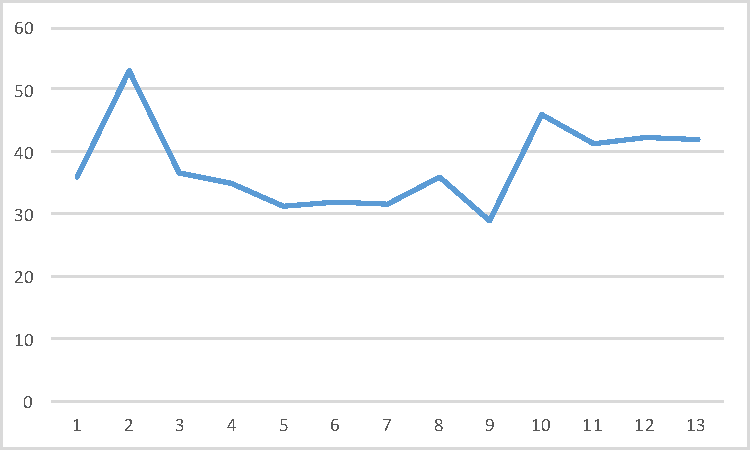
\includegraphics[width=1.0\textwidth]{src/images/evaluation/plots/01-book-pbmp-disc-1.pdf}
\caption[Chart of depth-discontinuity mask]{Depth-discontinuity mask applied on the book sequence with PBMP$_{disc,1px}$.}
\label{fig:eval-plots-pbmp-disc1}
\end{figure}

\noindent The graph shows also the correlation of the two metrics PBMP$_{disc,1px}$ and PBMP$_{noc,1px}$.
This means that each algorithm performs approximately the same way, either on depth-discontinuity areas or on non-occluded pixels with small positive displacement along the x-axis.
Concluding, the only algorithms which perform significantly worse than the others are the (2) OpenCV block matching implementation with filtering and (10) the simple OpenCV block matching implementation without filtering.
Although algorithm (4) MRF - ICM performs not as well as the others, it handles object borders at which depth-discontinuity occur more accurate than the other two outliers.
As this was just an example plot for depth-discontinuity areas, the other sequences behave the same way.

\subsubsection{Textureless regions}

\noindent The next Figure \ref{fig:eval-plots-pbmp-tex1} compares the amount of bad matching pixels in non-occluded regions with the textureless regions.
For this comparison, the tunnel scene of the Cambridge dataset was chosen.
It is clear to see that regions without textures, i.e. arbitrary surfaces are worse detectable than compared with textured objects.

\begin{figure}[h!]
\centering
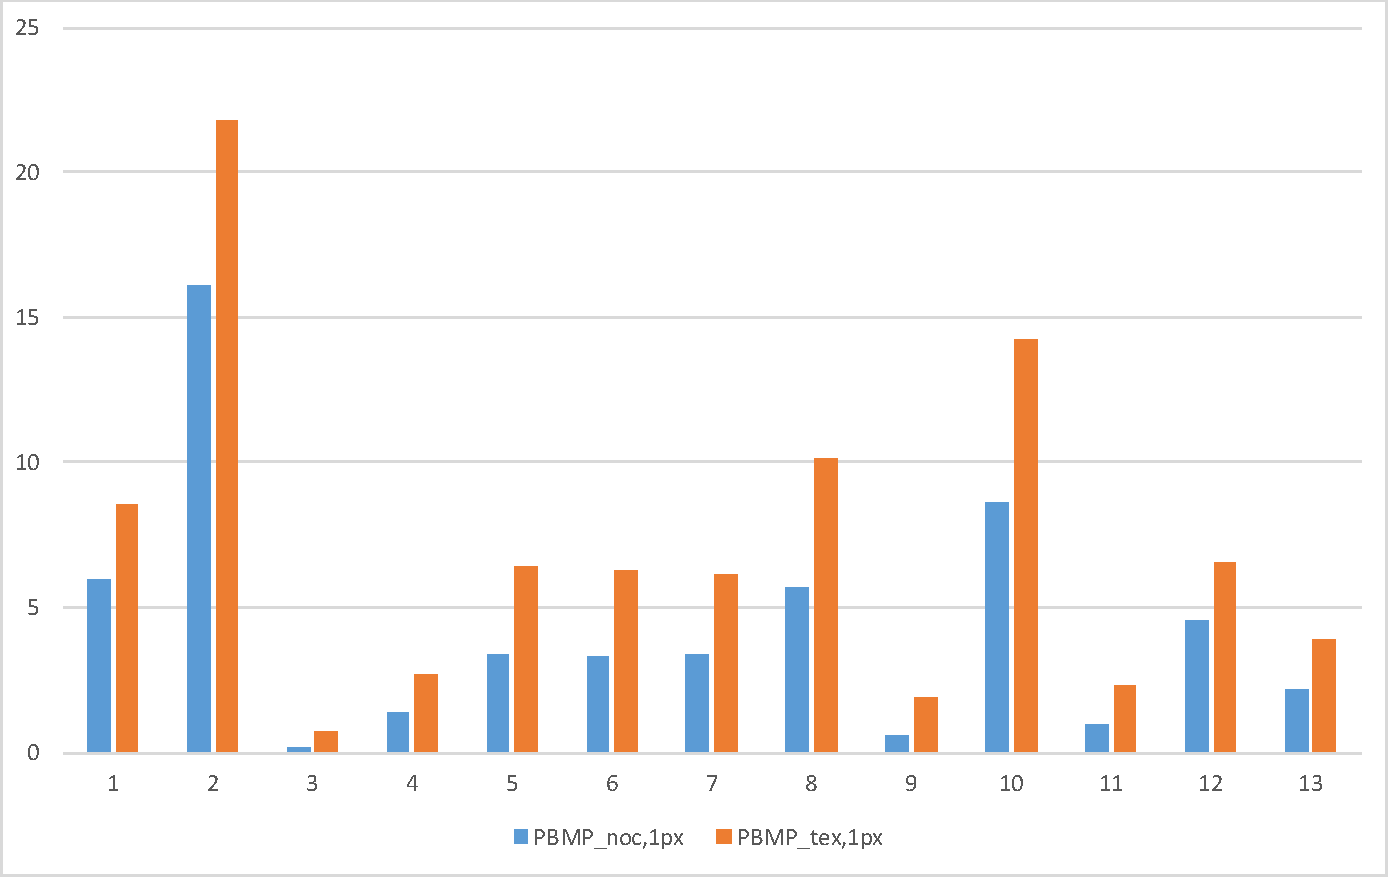
\includegraphics[width=1.0\textwidth]{src/images/evaluation/plots/05-tunnel-pbmp-tex-1.pdf}
\caption[Chart of textureless region mask]{Chart of textureless region mask applied on the tunnel sequence.}
\label{fig:eval-plots-pbmp-tex1}
\end{figure}

\noindent The percentage of bad matching pixels in textureless regions is nearly the same as overall in non-occluded areas, but with a positive displacement parallel to the x-axis.
It is also impressive that overall on average the ELAS algorithm yield to only 0.19\% of bad matching pixels in non-occluded regions PBMP$_{noc,1px}$.
In comparison, the worst algorithm, in this particular case the OpenCV block matcher implementation, resulted in PBMP$_{noc,1px}$ = 16.13\%.

\begin{table}[h!]
\centering
\scalebox{0.95}{
\begin{tabular}{l|rrrr}
  & RMSE$_{noc}$ & PBMP$_{noc,1px}$ & PBMP$_{noc,2px}$ & PBMP$_{noc,4px}$ \\ \hline
(3) ELAS & \cellcolor{green!50}0.36px & \cellcolor{green!50}0.19\% & \cellcolor{green!50}0.08\% & \cellcolor{green!50}0.04\% \\
(10) OpenCV - Simple BM & \cellcolor{red!50}5.82px & \cellcolor{red!50}8.60\% & \cellcolor{red!50}8.58\% & \cellcolor{red!50}8.56\% \\
(11) SNSM & 0.96px & 0.93\% & 0.71\% & 0.54\% \\
(12) SNSM STU & 1.02px & 4.53\% & 1.24\% & 0.73\% \\
(13) SNSM STW & 0.92px & 2.15\% & 0.79\% & 0.59\% \\
\hline
\end{tabular}
}
\caption[Result table for tunnel scene]{Result table for tunnel scene of Cambridge dataset}
\label{tab:eval:tex:tunnel:overview}
\end{table}

\noindent The SNSM also lead to feasible results which can be seen in Table \ref{tab:eval:tex:tunnel:overview}.
\newline\newline\noindent For a direct comparison of the visual outcome of the disparity maps, Figure \ref{fig:eval:heat:tunnel} depicts four images.
The left image with its ground-truth companion, the worst result of the OpenCV block matcher implementation and the best outcome yielded by ELAS.
ELAS seems to determine the disparity map in a nearly perfect manner but seems to struggle with the beginning shadow.

\begin{figure}[h!]
\centering
\begin{tabular}{cc}
\subfloat[left image]{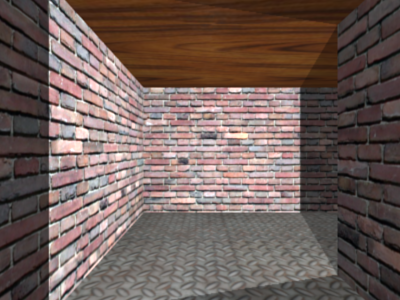
\includegraphics[width=0.45\textwidth]{src/images/evaluation/outliers2/tunnel-left.png}} &
\subfloat[ground-truth heatmap]{
\includegraphics[width=0.45\textwidth]{src/images/evaluation/outliers2/tunnel-ground-truth.png}} \\
\subfloat[outliers in OpenCV BM]{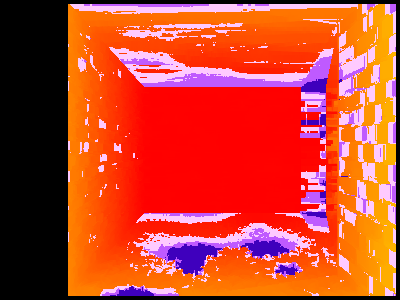
\includegraphics[width=0.45\textwidth]{src/images/evaluation/outliers2/tunnel-outliers-noc-2.png}} &
\subfloat[outliers in ELAS]{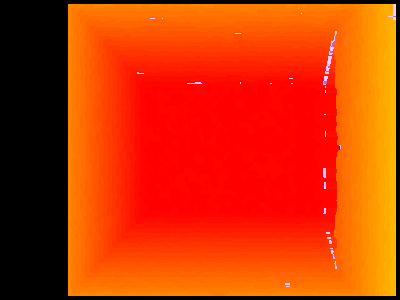
\includegraphics[width=0.45\textwidth]{src/images/evaluation/outliers2/tunnel-outliers-noc-3}}
\end{tabular}
\caption{Heatmaps for the tunnel scene}
\label{fig:eval:heat:tunnel}
\end{figure}

\noindent The SNSM led to feasible results in the tunnel scene, as can be seen in Table \ref{tab:eval:tex:tunnel:overview}.
The unweighted approach led to slightly worse overall results.
The interesting part here is the weighted approach of the SNSM implementation.
The RMSE$_{noc}$ improved whereas the PBMP$_{noc,1px}$ yield to shoddy results.
Considering both metrics, it shows that the naive spatiotemporal approach does not respect motion at all.
The slightly better RMSE$_{noc}$ feels a bit random in the overall evaluation.

\subsubsection{Salient regions}

Focusing on salient regions is a novel approach.
The distribution of salient regions does not follow any visual attracting regions.
According to \citeauthor{hou2007saliency} \citep{hou2007saliency}, the main idea is to extract the pixels which jump out of smooth curves, as they deserve most certainly the humans attention.
Their approach is implemented in the OpenCV library and no parameter can be set.
It is named static saliency, as only images are considered.
Thus, it is a pretty basic novel approach to create feasible masks with the static saliency.
The overall visual results are a bit confusing.
Figure \ref{fig:eval:sal:eg} shows two sample images and their corresponding computed saliency mask.
As can be seen in the figure, the static saliency approach in OpenCV yields to confusing results.
Although in both images, same parts, that are classified as salient regions, are comprehensible and understandable, some are not.

\begin{figure}[h!]
\centering
\begin{tabular}{cc}
\subfloat[image of book scene]{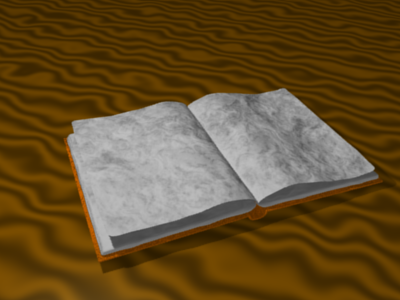
\includegraphics[width=0.45\textwidth]{src/images/evaluation/salient/left-book.png}} &
\subfloat[image of temple scene]{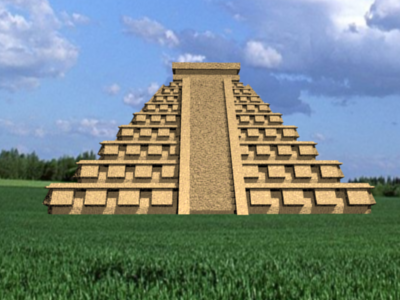
\includegraphics[width=0.45\textwidth]{src/images/evaluation/salient/left-temple.png}} \\
\subfloat[corresponding saliency mask]{
\includegraphics[width=0.45\textwidth]{src/images/evaluation/salient/salient-book.png}} &
\subfloat[corresponding saliency mask]{
\includegraphics[width=0.45\textwidth]{src/images/evaluation/salient/salient-temple.png}}
\end{tabular}
\caption{Examples for salient masks}
\label{fig:eval:sal:eg}
\end{figure}

\noindent The book as a whole is not recognized as salient as well as the stairs of the temple are left out completely.
The chart in Figure \ref{fig:eval-plots-pbmp-sal} depicts the application of the saliency mask to the book sequence.

\begin{figure}[h!]
\centering
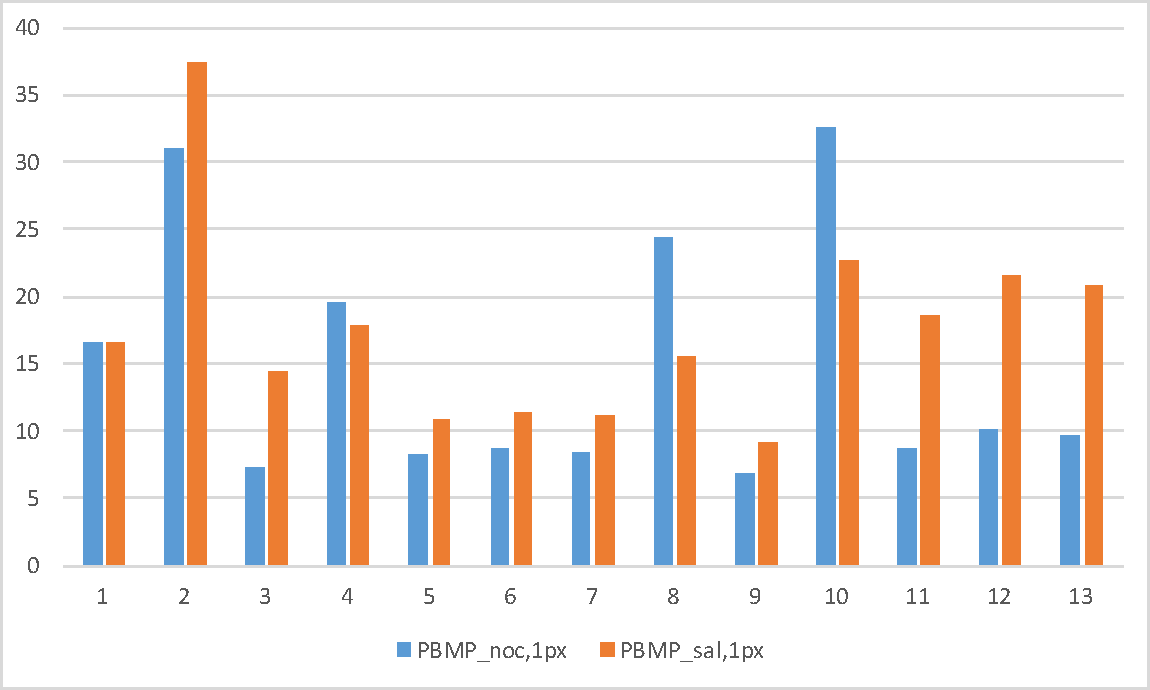
\includegraphics[width=1.0\textwidth]{src/images/evaluation/plots/01-book-pbmp-sal-1.pdf}
\caption[Chart of salient region mask]{Chart of salient region mask applied on the book sequence.}
\label{fig:eval-plots-pbmp-sal}
\end{figure}

\noindent The saliency mask has no real informative value.
There is no clear correlation identifiable.
In some cases, the saliency mask covers also depth-discontinuity areas and occluded areas.
Thus, it can yield to worse results than PBMP$_{noc,1px}$.
In other scenes of the Cambridge dataset, the results were similar to the book sequence.
Within high-resolution images, like the SVDDD dataset, the saliency mask looked even more unpredictable.
No clear salient regions were identifiable.
The assumption is that the algorithm, which is implemented in the OpenCV library is may be not capable of high-resolution images.
None the less, it could be shown, that the evaluation does not benefit from such a saliency mask.

\subsubsection{Outliers}

Beforehand, the investigation of outliers in a whole sequence of consecutive frames was mentioned.
During the evaluation, each sequence tended to have outliers.
To give an example, the book scene in combination with the (3) ELAS algorithm was chosen.
In this scene, two frames have significant more bad matched pixels than all the others, $23$ and $26$ although the margin is low.
The scenes shows a book.
During 41 frames one page will be turned over.

\begin{figure}[h!]
\centering
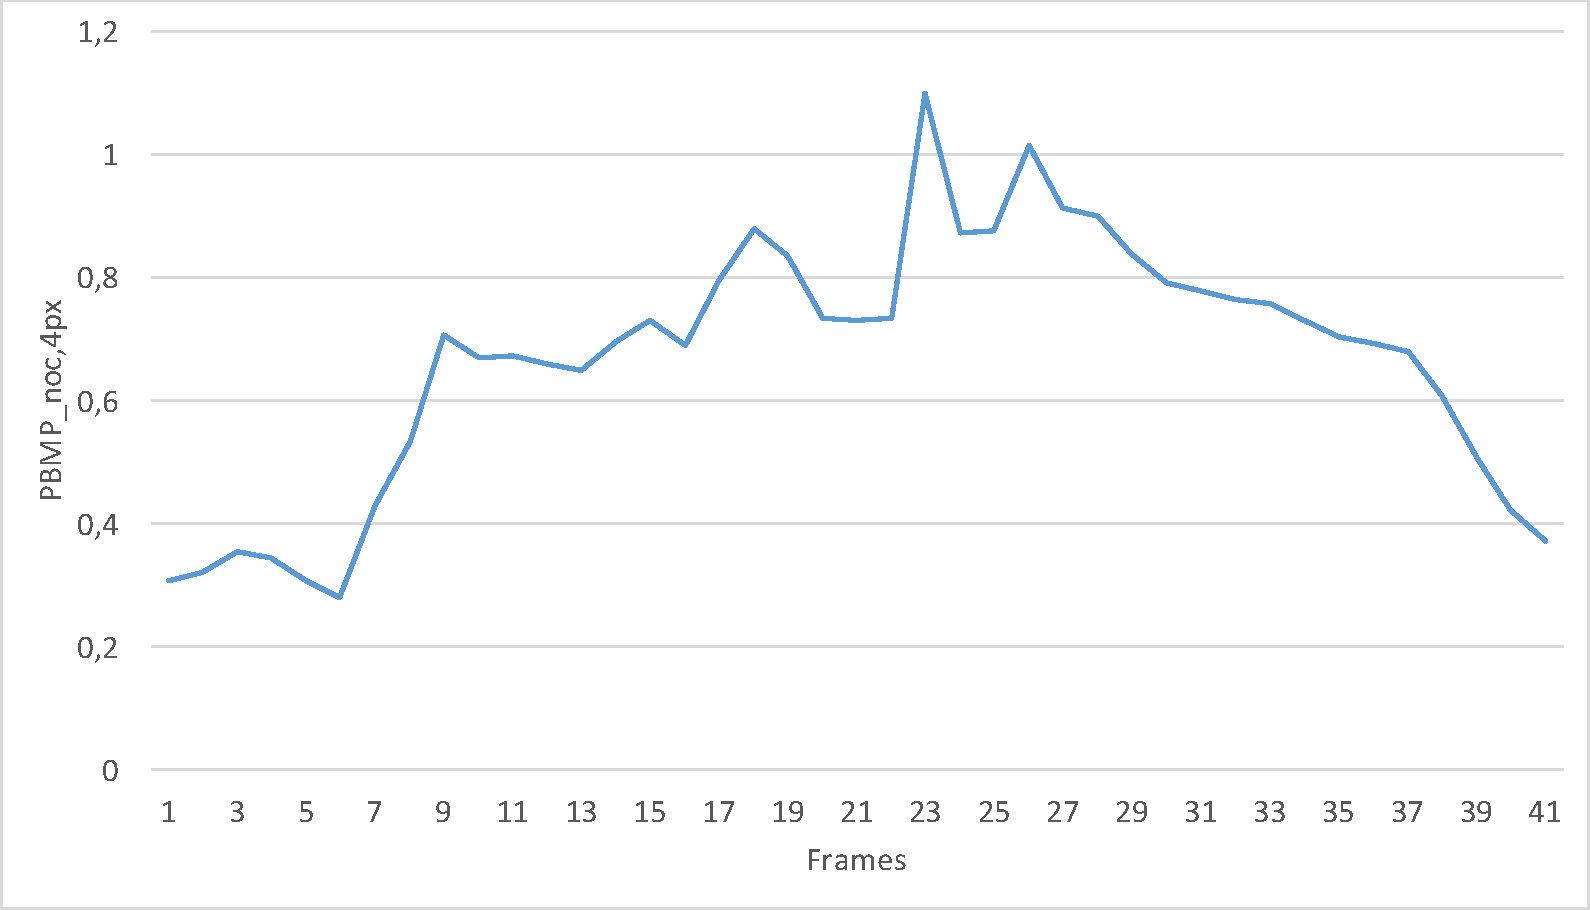
\includegraphics[width=1.0\textwidth]{src/images/evaluation/plots/01-book-general-outliers.pdf}
\caption[Chart of general outliers in a sequence]{Chart of general outliers in a sequence.}
\label{fig:eval-plots-outliers}
\end{figure}

\noindent The Figure \ref{fig:eval-plots-outliers} shows that in the beginning and in the end of the scene, exactly the point, in which the page is turned over and forms a flat surface with the book.
During the movement of the page, more object borders are created as the thin page forms a new object.
In frame $23$ and $26$ the turn over from one side to the other is made.
Thus, in exactly this two frames the amount of depth-discontinuity borders is the highest.
Figure \ref{fig:eval:out:eg} depicts these frames.
The increasing error at those object borders can be identified.
It is also clearly visible that Frame $23$ has the highest percentage  of bad matching pixels.

\begin{figure}[h!]
\centering
\begin{tabular}{ccc}
\subfloat[Frame 1]{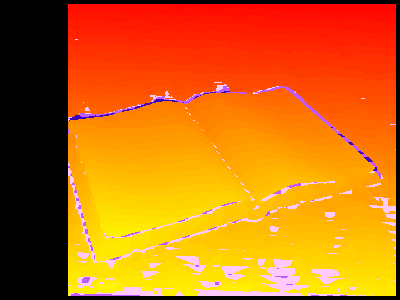
\includegraphics[width=0.3\textwidth]{src/images/evaluation/outliers/image0001.png}} &
\subfloat[Frame 23]{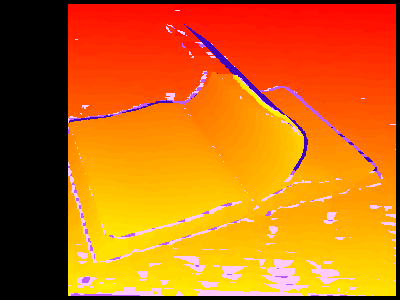
\includegraphics[width=0.3\textwidth]{src/images/evaluation/outliers/image0023.png}} &
\subfloat[Frame 26]{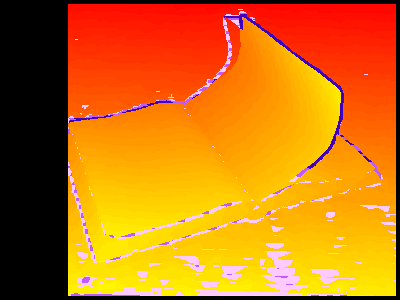
\includegraphics[width=0.3\textwidth]{src/images/evaluation/outliers/image0026.png}} \\
\end{tabular}
\caption[Examples for general outliers in a sequence]{Examples for general outliers in the book sequence. The disparity maps are computed with the (3) ELAS algorithm.}
\label{fig:eval:out:eg}
\end{figure}

\subsection{Impact of noise}

The impact of noise is an interesting and not often evaluated approach regarding disparity algorithms.
For this observation five different datasets were created with the image diminisher.
The Cambridge dataset was cloned and each image in this dataset was diminished with a newly created noise mask.
The noise mask was added on top of the image matrix.
Different values were chosen as mentioned in the measurement section.
For demonstration purpose, a plot, which contains all three $sigma^2$ values was chosen.
Figure \ref{fig:eval-plots-gn-overview} shows the impact of different $\sigma^2$ values for additive Gaussian noise on the computation of disparity algorithms.

\begin{figure}[h!]
\centering
\includegraphics[width=1.0\textwidth]{src/images/evaluation/plots/04-temple-gn-overview.pdf}
\caption[Chart of the impact of Gaussian noise]{Chart of the impact of different $\sigma^2$ values for additive Gaussian noise on the result of disparity algorithms focusing on P$_{noc,1px}$.}
\label{fig:eval-plots-gn-overview}
\end{figure}

\noindent Here, the tunnel scene was picked to demonstrate the impact of normal distributed noise.
Although, as mentioned beforehand in Chapter \ref{chap:impl}, the idea follows the methodology of \citeauthor{richardt2010real} \citep{richardt2010real}, it is not clear if additive Gaussian noise is an adequate image diminishing effect to simulate real scenery.
None the less, it is nice to see that all picked metrics correlate with each other.
The extent of the displacement along the x-axis depends on the amount of disturbing noise was added.
Figure \ref{fig:eval:gn:eg} depicts the first frame of the tunnel sequence with different noise degrees.
Added noise with a $sigma^2$ of $5$ does not seem to distract the visual appearance of the image.
None the less, it has a direct impact on the performance of disparity algorithms.
The degree of noise with a $\sigma^2$ of $15$ is visually noticeable.
One reason for that might be, that this type of noise may not appear in real-life while capturing a scene with a CCD sensor.
The approach follows the methodology of \citeauthor{richardt2010real} \citep{richardt2010real} but may not be suitable for simulating real scenery.
But, for the purpose of simulating an image, captured via CCD sensor, camera noise models exist \citep{liu2006noise}.
The approach with additive Gaussian noise changes every pixel in the image, by a different amount.
But an image, captured via CCD sensor, does not seem to have this pattern (cf. \citep{liu2006noise}).
Changing every pixel, even by a small amount means that the calculated matching cost may differ largely.
This is of course depending on other factors, such as window size and which matching cost formula is applied.
The assumption remains, that additive Gaussian noise may not be a good choice to simulate real scenery and to measure the in uence on disparity algorithms.

\begin{figure}[h!]
\centering
\begin{tabular}{cc}
\subfloat[temple frame]{\includegraphics[width=0.45\textwidth]{src/images/evaluation/outliers-gn/image0001.png}} &
\subfloat[$\sigma^2=5$]{\includegraphics[width=0.45\textwidth]{src/images/evaluation/outliers-gn/image0001-gn5.png}} \\
\subfloat[$\sigma^2=10$]{\includegraphics[width=0.45\textwidth]{src/images/evaluation/outliers-gn/image0001-gn10.png}} &
\subfloat[$\sigma^2=15$]{\includegraphics[width=0.45\textwidth]{src/images/evaluation/outliers-gn/image0001-gn15.png}}
\end{tabular}
\caption{Examples for image diminishing effects with Gaussian noise}
\label{fig:eval:gn:eg}
\end{figure}

\noindent The upcoming subsection also deals with image diminishing effects, in this case video compression.

\subsection{Impact of video compression}

The impact of video compression is an interesting and novel approach.
High-resolution videos, due to its nature, are not shipped for television as uncompressed raw data or even lossless compressed.
As seen in the Chapter \ref{chap:related}, there are different applications for disparity algorithms.
One outpointed need is the remapping of disparity for different screen sizes.
If this can not happen on raw data, for instance the data is missing and only the compressed version is available, the influence of video compression on the outcome of disparity algorithms is observed.
\noindent For this observation five different datasets were created with the image diminisher.
As underlying video codec H.265 was chosen because it is currently the most efficient video compression technique.
The recommended default parameter for H.265, the constant rate factor (CRF) is $28$.
It ranges from $0-51$, whereas $0$ represents lossless and $51$ the worst possible compression.
$0, 14, 28, 40, 51$ were chosen with $14$ and $40$ as additionally in-between parameters.
$0$ and $51$ were left out, as the result is too visually distracting for the viewer with $51$ and $0$ is lossless.
Thus, the observed values are $14, 28, 40$.

\begin{figure}[h!]
\centering
\begin{tabular}{ccc}
\subfloat[book, CRF = 14]{\includegraphics[width=0.3\textwidth]{src/images/evaluation/outliers-vc/book-image0022-vc14.png}} &
\subfloat[book, CRF = 28]{\includegraphics[width=0.3\textwidth]{src/images/evaluation/outliers-vc/book-image0022-vc28.png}} &
\subfloat[book, CRF = 40]{\includegraphics[width=0.3\textwidth]{src/images/evaluation/outliers-vc/book-image0022-vc40.png}} \\
\subfloat[tanks, CRF = 14]{\includegraphics[width=0.3\textwidth]{src/images/evaluation/outliers-vc/tanks-image0023-vc14.png}} &
\subfloat[tanks, CRF = 28]{\includegraphics[width=0.3\textwidth]{src/images/evaluation/outliers-vc/tanks-image0023-vc28.png}} &
\subfloat[tanks, CRF = 40]{\includegraphics[width=0.3\textwidth]{src/images/evaluation/outliers-vc/tanks-image0023-vc40.png}} \\
\end{tabular}
\caption[Examples for image diminishing effects with video compression]{Examples for image diminishing effects caused by video compression artifacts of the H.265 codec in combination with different values for CRF.}
\label{fig:eval:vc:eg}
\end{figure}

\noindent Figure \ref{fig:eval:vc:eg} depicts the effect of different CRF values using H.265.
It is clearly visible that a CRF with $14$ leads to feasible results regarding the experience for viewers.
A CRF with $28$ and $40$ lead to more distracting artifacts.
Figure \ref{fig:eval-plots-pbmp-noc1-vc} illustrates the correlation of the H.265 CRF and PBMP$_{noc,1px}$.
Even the lowest value in test series, $14$ leads to a huge amount of bad matching pixels.
A CRF with $28$ seems to as hard as $14$ for disparity algorithm, as the amount of bad matching pixels is nearly identical with the amount of $14$.

\begin{figure}[h!]
\centering
\includegraphics[width=1.0\textwidth]{src/images/evaluation/plots/03-tank-pbmp-noc-1-vc.pdf}
\caption[Chart of the impact of video compression]{Chart of the impact of different CRF values for H.265 video compression on the result of disparity algorithms focusing on PBMP$_{noc,1px}$.}
\label{fig:eval-plots-pbmp-noc1-vc}
\end{figure}

\noindent Figure \ref{fig:eval:vc:eg2} depicts the computed disparity maps after diminishing the whole scene with a CRF value of $40$.
Many disparity information seem to be lost.
The structure of the fire pipe of the right tank is still visible and the disparity information are valid within a threshold of $1px$.
The rest feels a bit random.
\newline\newline\noindent Talking about SNSM, it lead to better results than most of the other algorithms.
In the tank sequence, (11) SNSM achieved PBMP$_{noc,1px}$ = 80.72\% where as (8) MRF - BP BPM achieved 82.45\%, which led to superior results beforehand.
The unweighted and weighted approach were able to improve this result to 75.04\% and respectively 75.58\%.

\begin{figure}[h!]
\centering
\begin{tabular}{ccc}
\subfloat[(3) ELAS outliers]{\includegraphics[width=0.3\textwidth]{src/images/evaluation/outliers-vc/image0023-heatmap-outliers-3.png}} &
\subfloat[(5) MRF GC Swap outliers]{\includegraphics[width=0.3\textwidth]{src/images/evaluation/outliers-vc/image0023-heatmap-outliers-5.png}} &
\subfloat[(13) SNSM STW]{\includegraphics[width=0.3\textwidth]{src/images/evaluation/outliers-vc/image0023-heatmap-outliers-13.png}} \\
\end{tabular}
\caption[Example of computed disparity maps with video compression]{Example of computed disparity maps with video compression. CRF is set to $40$. Frame 23 of the tanks scene.}
\label{fig:eval:vc:eg2}
\end{figure}

\subsection{Runtime}

Talking about runtime, the results differ vastly.
Figure \ref{fig:eval-plots-runtime} illustrates the different runtimes in mean over all sequences of the Cambridge dataset.
This should provide a solid overview.
It is clear to see that four variants run fast, i.e. have a low runtime.
This is true for the local methods, as well as ELAS.
The global methods need much more time to approximate the energy function.
\newline\newline\noindent Especially the algorithm variants of belief propagation needed much time.
Throughout the whole evaluation, (8) MRF - BP BPM led to the best results, compared with other global methods.
The runtime is according to algorithm (7) MRF - BP TRWS and (9) MRF - BP BPM the lowest.
Comparing with other results, which were outlined in the sections before, the runtime is not justified as the longer an algorithm runs does not automatically yield to better results.
\newline\newline\noindent The (11) SNSM is the worst local method focusing on the runtime in comparison with (1), (2) and (10), which are all OpenCV implementations of block matching algorithms.
This may result as the whole disparity space image is calculated beforehand the disparity maps are computed.
So the runtime of the SNSM is basically the runtime for the whole scene divided through the amount of frames.
Both variants, the (12) SNSM-STU and (13) SNSM-STW are dealing with the same information in the same way besides the assembly of the matching cost.
But this should not affect the runtime at all, so it is also clearly to see, that a certain deviation of the runtime has to be kept in mind.
\newline\newline\noindent ELAS outperformed in many times all the other algorithms according to PBMP$_{noc}$.
The runtime is feasible for real-time applications but slightly worse than simple local methods, like the OpenCV block matcher implementation.
Although, it has to be kept in mind, as outlined in Chapter \ref{chap:impl}, that ELAS is a library which comes with a front-end and an internal image library.
Both can be the origin for the runtime being worse than simple block-matching algorithm.
For an accurate comparison which approach is faster, both should be implemented utilizing the same underlying image library.

\begin{figure}[h!]
\centering
\includegraphics[width=1.0\textwidth]{src/images/evaluation/plots/runtime.pdf}
\caption[Comparison of the runtime of different disparity algorithms]{Comparison of the runtime of different disparity algorithms}
\label{fig:eval-plots-runtime}
\end{figure}

\subsection{SVDDD}

The SVDDD dataset from the department of Praktische Informatik IV\footnote{\url{http://ls.fmi.uni-mannheim.de/de/pi4/}} was evaluated as well.
During this thesis, the dataset ran through several iterations as more and more problems arose during the evaluation.
In addition, some algorithms were not able to process high-resolution stereo images.
Thus, it is separated from the other results.
\newline\newline\noindent The initially evaluated scenes led to strange results.
Some areas were computed correctly but some areas were completely off.
One major point, which can lead to such strange, defective results, is negative disparity.
Most of the algorithms expect that disparity values range from $0-d_{max}$.
Even a small amount of negative disparity can conduct to a result, which is slightly off, i.e. three or four pixels.
Looking at PBMP$_{1px}$ , which can yield to nearly $50\%$.
An example can be seen in Figure \ref{fig:outliers-rabbit-svddd}, illustrating two images.
In the left image about $10\%$ pixels overall contains slightly negative disparity whereas in the right image, the disparity ranges from $0-59$.

\begin{figure}[h!]
\centering
\begin{tabular}{ccc}
\subfloat[Negative disparity]{\includegraphics[width=0.48\textwidth]{src/images/evaluation/02-rabbit-neg-elas.png}} &
\subfloat[Only positive disparity]{\includegraphics[width=0.48\textwidth]{src/images/evaluation/02-rabbit-elas.png}} &
\end{tabular}
\caption[Computed disparity map with negative disparity]{Comparison of computed disparity maps regarding negative disparity.}
\label{fig:outliers-rabbit-svddd}
\end{figure}

\noindent Another challenge of high-resolution datasets is the huge computational power, which is necessary to compute disparity maps for them.
The BP algorithms would have needed about $52 GB$ of memory to calculate the scenes for $d_{max} = 64$ as the labels for all possible states have to be created and stored in memory.
Also, the SNSM wanted to allocate about $35 GB$ of memory as the disparity space image is computed \textit{a priori} before the actual calculation of the disparity maps takes place.
The runtime also gives a feeling how computational powerful and complex it is, to perform a disparity estimation on high-resolution stereo images.
Summing up, the MRF BP algorithms as well as the SNSM were excluded from the evaluation of the SVDDD dataset.

\begin{table}[h!]
\centering
\scalebox{1.0}{
\begin{tabular}{l|rrrrrr}
  & 1 & 2 & 3 & 4 & 5 & 6 \\ \hline
02-rabbit-neg & 58.62\% & \cellcolor{red!50}61.51\% & 59.99\% & 60.58\% & \cellcolor{green!50}57.12\% & 57.13\% \\
02-rabbit & 1.68\% & \cellcolor{red!50}4.31\% & 2.98\% & 3.82\% & \cellcolor{green!50}0.65\% & 0.68\% \\
03-apple & 1.69\% & \cellcolor{red!50}4.10\% & 3.11\% & 3.44\% & \cellcolor{green!50}0.63\% & 0.65\% \\ \hline
$\varnothing$ (w/o neg) & 1.69\% & \cellcolor{red!50}4.21\% & 3.05\% & 3.63\% & \cellcolor{green!50}0.64\% & 0.67\%
\end{tabular}
}
\caption[Result table for general performance of SVDDD]{Result table for general performance of SVDDD, focusing on PBMP$_{noc,1px}$}
\label{tab:svddd-performance}
\end{table}

\noindent Table \ref{tab:svddd-performance} contains the mean results of the SVDDD dataset.
The best result is achieved with the MRF GC Expansion algorithm, which only led to $0.64\%$ of bad matching pixels in all scenes which is quite impressive for both, the scenes and the algorithms.
OpenCV SGBM and ELAS also lead to good results.
Comparing the runtime of such high-resolution scenes, the (2) OpenCV BM clearly outperforms the others.
Taking the general performance into account, OpenCV SGBM and ELAS both yield to feasible results.
For real-time applications ELAS stands out against the other algorithms.
Taking both, the overall performance and the runtime into account, ELAS performs best.
In Figures \ref{fig:eval-svddd-plot-rabbit} and \ref{fig:eval-svddd-plot-apple}, it is clearly to see that ELAS also performs better than the other local methods regarding PBMP$_{noc,4px}$.

\begin{figure}[h!]
\centering
\includegraphics[width=1.0\textwidth]{src/images/evaluation/svddd/02-rabbit-plot.pdf}
\caption[Performance of SVDDD rabbit scene]{Performance of SVDDD rabbit scene}
\label{fig:eval-svddd-plot-rabbit}
\end{figure}

\noindent Both scenes, rabbit and apple performed pretty reasonable.
In direct comparison with the Cambridge datasets, the results are better.
The Cambridge scenes are unrealistic constructed in comparison to the Big Buck Bunny project as they contain a lot of repeating objects and arbitrary textures.
Even the tunnel scenery contains many identical looking bricks.
The literature states, that those textures are error-prone areas, this could be a reason for the better performing SVDDD.
The coloring of the scenes in the Cambridge dataset is very even distributed whereas the SVDDD dataset contains different colors in each scene.
Some scenes of the Cambridge dataset led to worse result than the others, especially the street scene performed best, which supports the assumption, that the result rely on the composition of the scenery.
In the beginning, the assumption arose, that the fine hair textures may be problematic.
This is not the case.
The computed disparity map lack of accuracy near depth-discontinuity areas, but fine-grained structures were not problematic at all.

\begin{figure}[h!]
\centering
\includegraphics[width=1.0\textwidth]{src/images/evaluation/svddd/03-apple-plot.pdf}
\caption[Performance of SVDDD apple scene]{Performance of SVDDD apple scene}
\label{fig:eval-svddd-plot-apple}
\end{figure}

\noindent Focusing on the runtime, which is illustrated in Table \ref{tab:svddd-runtime}, the fastest algorithm is again the OpenCV BM implementation.
But the huge gap between (2) ELAS, (3) OpenCV BM and the others is noticeable.
ELAS seems to be a pretty solid approach regarding runtime and overall performance of disparity estimation.
The best results were achieved by the global methods, which pretty astonishing results of PBMP$_{noc,1px} < 1\%$.
The runtime was very bad with nearly 10 minutes to compute one single disparity map.
It has to be kept in mind, that the computation depends heavily on the underlying computing engine (CPU or GPU) and also the implementation.
Also, in difference to the Cambridge dataset, the SVDDD dataset led to endless iterations in the Middlebury library.
The Middlebury library is kept to a maximum of 500 iterations, which is not adjustable.
The SVDDD dataset always needed the whole iterations, which may be the reason for such a long runtime.
A reason for that can be the high resolution of the dataset.

\begin{table}[h!]
\centering
\scalebox{0.9}{
\begin{tabular}{l|rrrrrr}
  & 1 & 2 & 3 & 4 & 5 & 6 \\ \hline
02-rabbit-neg & 6550 ms & \cellcolor{green!50}817 ms & 1923 ms & 11796 ms & 300939 ms & \cellcolor{red!50}544833 ms \\
02-rabbit & 4402 ms & \cellcolor{green!50}465 ms & 1000 ms & 20141 ms & 420835 ms & \cellcolor{red!50}617998 ms \\
03-apple & 4541 ms & \cellcolor{green!50}467 ms & 984 ms & 16063 ms & 384221 ms & \cellcolor{red!50}575137 ms \\ \hline
$\varnothing$ & 5164 ms & \cellcolor{green!50}583 ms & 1302 ms & 16000 ms & 368665 ms & \cellcolor{red!50}579323 ms
\end{tabular}
}
\caption[Result table for runtime of SVDDD]{Result table for runtime of SVDDD}
\label{tab:svddd-runtime}
\end{table}

\section{Discussion}

In this section, the result seen before are summarized and discussed.
The general performance of the integrated algorithms in comparison with the simple naive stereo matcher (SNSM) is interesting.
The outcome of the comparison is, that in general local methods are faster than global methods but the quality benefit of the disparity map may not be high.
Although, this depends heavily on the use-case, only one global method, the (9) MRF - BP BPM was really superior.
SNSM is on a level playing field with other global methods, and even outperforms some, like (3) MRF ICM and (8) MRF - BP BPS.
Taking the spatiotemporal context into account yields overall to better results, but still lacks of respecting the motion of objects.
Thus, the result may be a bit random regarding this particular case, as mentioned beforehand in Chapter \ref{chap:impl}.
The masks are granting another perspective on the performance of disparity algorithms, but only the depth-discontinuity as well as the non-occluded pixel mask seem to give a real overall benefit.
The saliency mask seems to bit more random as most of the salient regions are not marked correctly whereupon the room for interpretation when it comes to saliency has to be kept in mind.
\newline\newline\noindent The results regarding Gaussian noise differ from the results, which \citeauthor{richardt2010real} \citep{richardt2010real} achieved.
Here, a much lower $\sigma^2$ led to defective results.
As every pixel gets changed according to the normal distribution and additionally, for each image a different noise matrix was calculated to avoid pattern matching, the stereo image gets disturbed in an unnatural way.
\citeauthor{richardt2010real} added additive Gaussian noise to simulate a more natural, real scenery.
Gaussian noise is a part of sensor noise, but a small one.
To simulate such real scenery, a more realistic model should be created.
For the purpose of simulating an image, captured via CCD sensor, camera noise models exist \citep{liu2006noise}.
Such complex noise models are difficult to create, but maybe lead to much more feasible results.
However, it could be shown that a small amount of normal distributed noise lead to false disparity information.
The small amount of informative value is may be at random computed.
\newline\newline\noindent With testing the interference of video compression, a novel approach was shown.
The outcome of the approach is, that even a small amount of video compression artifacts lead to a lot of mismatched pixels, although the artifacts are not clearly visible.
As two parameters are correlating directly and the change of the CRF from $14$ to $28$ did not change the overall result, it may be the case, that disparity algorithms struggle with a small amount of noise until a certain level.
The jump from about 10\% of bad matching pixels to nearly 60\% at the first tested step is huge.
In case of disparity remapping, as discussed in Chapter \ref{chap:related}, it does not make any sense to count on compressed video material.
The resulting disparity maps seem to be too much disturbed regarding the overall performance.
\newline\newline\noindent Taking the runtime into account, the information taken out of the literature were confirmed.
Global methods tend to run pretty long whereas local methods are more for real-time applications.
Here, ELAS established itself as a surprise candidate.
The overall performance combined with the runtime is good.
The results towards object borders are accurate.
Depending on the image resolution, global methods struggle with high-resolution images whereas ELAS performed pretty well.
Global methods tend to run pretty long, nearly 1000 times the runtime of local methods.
\newline\newline\noindent The last part of the evaluation was to benchmark the SVDDD dataset of the department of Praktische Informatik IV\footnote{\url{http://ls.fmi.uni-mannheim.de/de/pi4/}}.
After initial problems with the range of disparity values as well as some ground-truth disparity maps contained unfeasible values, two final scenes were constructed and could be evaluated.
Both scenes performed very good along all algorithms.
Worth mentioning is also the achieved performance in comparison with the Cambridge dataset.
SVDDD led to notable better results.
This may come from the composition of both scenes, as much more different textures and colors are included.
Focusing on the runtime of the SVDDD dataset and feasibility of applying disparity algorithms on it, the computational limitations became noticeable.
The belief propagations as well as the SNSM implementation were in need of too much memory.
This may come from bad implementation as well as inappropriate parameters.
The parameters of the Middlebury MRF library were not adjustable.
Thus, this could not be investigated further more.
None the less, the other algorithms drew the bigger picture with the main outcome, that the OpenCV SGBM implementation as well as ELAS performed best.


\chapter{Conclusion}
\label{chap:conclusion}

The work described in this thesis has been concerned with the comparison of disparity algorithms.
For this purpose, evaluation methods were introduced and integrated.
As stereoscopic datasets focusing on videos are rarely spread, the used ones for the evaluation were also introduced.
Additionally, a simple stereo matcher focusing on videos was implemented and thus described.
The following section recaps this in more detail and furthermore a future outlook is given.

\section{Thesis summary}

\begin{itemize}
  \item What the thesis brought with each chapter.
  \item One small paragraph regarding one disparity algorithm.
  \item One small paragraph regarding dataset of the chair.
  \item What the main result of the evaluation.
\end{itemize}

\noindent The following modules were actually implemented:

\begin{itemize}
  \item Reader for the PFM file format.
  \item Python scripts for evaluation.
  \item Shell scripts for creating docker containers and distribute the work among different server instances.
  \item Evaluation processor based on OpenCV for stereoscopic videos compared with their ground-truth companion.
  \item A simple stereo matcher targeting videos by holding a spatiotemporal context.
  \item An image diminisher utilizing FFmpeg to simulate noise and video compression artifacts.
\end{itemize}

\noindent Summarize the results of the evaluation.

%todo add recommendations for svddd dataset

\section{Outlook and future work}

A few thoughts on possible future work are outlined.
The thoughts are split in low- and high-level, from a technical perspective.
Low-level items are focused towards underlying methods of disparity algorithms, whereas high-level items focus on the bigger picture and tools which may help in developing stereo matcher.

\begin{itemize}
  \item Neuronal networks \citep{olshausen1996emergence}
  \item Other matching cost calculation methods \citep{hermann2010gradient}.
  \item Focus more on how humans experience depth? \citep{deangelis1995neuronal}
\end{itemize}

\begin{itemize}
  \item Real-time availability
  \item higher resolution
  \item What's on the market, like multi-view?
  \item Provide more real-world ground truth disparity maps \citep{kondermann2015stereo, Geiger2011IV}.
\end{itemize}


% End of main part
% ---------------------------------

% ---------------------------------
% Begin of appendix
\appendix
% Appendix chapters are optional. Use it if you have very long tables or additional figures that
% do not belong to the main text.
% \chapter{Tables}

% Remove this from the final document
% \chapter{Checklist}
\label{chap:appendix:checklist}
Use the following list to check if you have followed the hints from this document in your work.
Refer to \cref{chap:introduction} for more information on the items.

\tabulinesep=2.5mm
% tabu allows to use relative width specifier: Use X[<ratio>] to specify the width of a column. In
% this example, the table is divided into 20 parts that are spread over the three columns.
\begin{longtabu} to \textwidth {|X[1]|X[17]|X[2]|}
% Begin header on first page
\caption[Formatting checklist]{The checklist for correctly formatted and prettier documents.}
\label{tab:checklist}
\\
\hline
\endfirsthead
% End header on first page

% Begin header on consecutive pages
\caption[]{Table continued.}
\\
\hline
\endhead
% End header on consecutive pages

% Begin footer
\multicolumn{3}{c}{Table is continued on the next page.} \\
\endfoot
% End footer

% Begin footer on last page
\endlastfoot
% End footer on last page

% Begin content
1. & Check for incorrect/missing citations (\emph{[?]}) or references (\emph{??}). & \\
\hline
2. & Remove all \LaTeX{} errors and underfull/overfull boxes. & \\
\hline
3. & Make sure to use a consistent encoding for your \TeX{} files, especially for special characters (ä, ö, ü, ß, \dots). & \\
\hline
4. & Format your \textsc{Bib}\TeX{} document: Check if the information is correct and complete for each entry. Pay notice to warnings when running  the \texttt{bibtex} command.& \\
\hline
5. & Add access dates to online sources in your bibliography (see \texttt{library.bib}) or in footnotes. & \\
\hline
6. & Run a spell checker over your document (included with some \LaTeX{} editors). & \\
\hline
7. & Place figures or tables in the \TeX{} file at the end of the paragraph you are referring to them in the text (\texttt{\textbackslash{}ref}). & \\
\hline
8. & Use the correct format for quotation marks (\emph{``x''} or \emph{\glqq{}x\grqq{}}). & \\
\hline
9. & Use the correct format for separating paragraphs (one empty line). Manual line breaks (\texttt{\textbackslash{}\textbackslash}) should be avoided. & \\
\hline
10. & Use the correct form of dashes (-, --, ---). & \\
\hline
11. & Separate citations at the end of sentences/paragraphs with a small whitespace (\texttt{\~}). & \\
\hline
12. & Name sources of images/figures you did not create yourself in the description (\emph{Source: [X]}). & \\
\hline
13. & Use the short form of captions for List of Figures, Tables, etc. (\texttt{caption[<short>]\{<long>\}}). & \\
\hline
14. & If you print your work double-sided (recommended for bachelor and master thesis) remove the \texttt{oneside} option from the document class. & \\
\hline
15. & Make sure to use high-quality figures and images that are readable both in the digital and the printed version. & \\
\hline
16. & If you include the declaration of honor do not forget to sign it. & \\
\hline
% End content
\end{longtabu}

\backmatter

\bibliography{library}

\sloppy
\printglossary
\fussy

\declarationofhonorchap

Hiermit versichere ich, dass diese Arbeit von mir pers{\"o}nlich verfasst wurde und dass ich keinerlei fremde Hilfe in Anspruch genommen habe. Ebenso versichere ich, dass diese Arbeit oder Teile daraus weder von mir selbst noch von anderen als Leistungsnachweise andernorts eingereicht wurden. W{\"o}rtliche oder sinngem{\"a}ße {\"U}bernahmen aus anderen Schriften und Ver{\"o}ffentlichungen in gedruckter oder elektronischer Form sind gekennzeichnet. S{\"a}mtliche Sekund{\"a}rliteratur und sonstige Quellen sind nachgewiesen und in der Bibliographie aufgef{\"u}hrt. Das Gleiche gilt f{\"u}r graphische Darstellungen und Bilder sowie f{\"u}r alle Internet-Quellen.
Ich bin ferner damit einverstanden, dass meine Arbeit zum Zwecke eines Plagiatsabgleichs in elektronischer Form anonymisiert versendet und gespeichert werden kann.

\vspace{1cm}
\noindent
\insertcitydate{Mannheim}{Mai 2016}

\vspace{1.5cm}
\noindent
\insertauthor


% Consult your supervisor about the following declaration of assignment.
\begin{lang-de}
\chapter{Abtretungserklärung}
Hinsichtlich meiner Abschlussarbeit mit dem Titel \emph{\glqq{}\begin{lang-main}\inserttitle\end{lang-main}\grqq{}} räume ich der Universität Mannheim\fshyp{}Lehrstuhl für Praktische Informatik IV, Prof.\ Dr.\ Wolfgang Effelsberg, umfassende, ausschließliche unbefristete und unbeschränkte Nutzungsrechte an den entstandenen Arbeitsergebnissen ein.
Die Abtretung umfasst das Recht auf Nutzung der Arbeitsergebnisse in Forschung und Lehre, das Recht der Vervielfältigung, Verbreitung und Übersetzung sowie das Recht zur Bearbeitung und Änderung inklusive Nutzung der dabei entstehenden Ergebnisse, sowie das Recht zur Weiterübertragung auf Dritte.
\newline\newline\noindent Solange von mir erstellte Ergebnisse in der ursprünglichen oder in überarbeiteter Form verwendet werden, werde ich nach Maßgabe des Urheberrechts als Co\hyp{}Autor namentlich genannt.
Eine gewerbliche Nutzung ist von dieser Abtretung nicht mit umfasst.

\vspace{1cm}
\noindent
\insertcitydate{Mannheim}{3. Mai 2016}

\vspace{1.5cm}
\noindent
\insertauthor
\end{lang-de}

% End of appendix
% ---------------------------------

\end{document}
